

\documentclass[journal]{IEEEtran}

%%%%%%%%%%%%%%%%%%%%%%%%%%%%%%%%%%%%%%%%%%%%%%%%%%%%%%%%%%%%%%

\usepackage[italian]{babel}

% *** CITATION PACKAGES ***
\usepackage[style=ieee]{biblatex} 
\bibliography{digital.bib}    %your file created using JabRef
\usepackage{hyperref}

% *** MATH PACKAGES ***
\usepackage{amsmath}
 \usepackage{multirow}

% *** PDF, URL AND HYPERLINK PACKAGES ***
\usepackage{url}
% correct bad hyphenation here
\hyphenation{op-tical net-works semi-conduc-tor}
\usepackage{graphicx}  %needed to include png, eps figures
\usepackage{float}  % used to fix location of images i.e.\begin{figure}[H]

\usepackage{csquotes} % correzione errore compilazione
\usepackage[table]{xcolor}

%%%%%%%%%%%%%%%%%%%%%%%%%%%%%%%%%%%%%%%%%%%%%%%%%%%%%%%%%%%%%


\begin{document}

% paper title
\title{Laboratorio di elettronica digitale\\ 
%\small{1 gennaio 2020}
}

% author names 
\author{\begin{center}Matteo Barbagiovanni\textsuperscript{1},
        Stefano Barbero\textsuperscript{2},
        Federico Malnati\textsuperscript{3},
        Valerio Pagliarino\textsuperscript{4},
        {\small \\
        \textsuperscript{1}
        matteo.barbagiovanni@edu.unito.it -
        \textsuperscript{2}
        stefano.barbero376@edu.unito.it
        \textsuperscript{3}
        federico.malnati@edu.unito.it -
        \textsuperscript{4}
        valerio.pagliarino@edu.unito.it}
        \end{center}}% <-this % stops a space
        
% The report headers
\markboth{Università degli Studi di Torino - C.d.L. Triennale in Fisica - 19/11/21 - A.A. 2021-2022    \quad   \quad \quad \quad   \quad \quad \quad  \quad   \quad \quad \quad   \quad \quad LABORATORIO DI ELETTRONICA \quad \quad }%do not delete next lines
{Shell \MakeLowercase{\textit{et al.}}: Bare Demo of IEEEtran.cls for IEEE Journals}

% make the title area
\maketitle


%%%%%%%%%%%%%%%%%%%%%%%%%%%%%%%%%%%%%%%%%%%%%%%%%%%%%%%%%%%%%
%% Introduzione 
%%%%%%%%%%%%%%%%%%%%%%%%%%%%%%%%%%%%%%%%%%%%%%%%%%%%%%%%%%%%%

\begin{abstract} 
Dopo aver analizzato i principali circuiti analogici che consentono l'amplificazione e il condizionamento dei segnali, in questa seconda relazione di laboratorio si studieranno alcune tecniche di elettronica digitale con l'obiettivo di realizzare un convertitore ADC (Analog to Digital Converter) ad approssimazioni successive, analizzando la catena del segnale dall'ingresso analogico fino alla memorizzazione dei dati su scheda di memoria. Inizialmente, dopo aver introdotto la famiglia di integrati digitali 7400 che verrà utilizzata, verranno prese in esame alcune funzioni logiche fondamentali come le porte AND, NAND, NOT, i flip-flop di tipo set-reset e J-K di cui verranno studiate le tabelle di verità e talvolta le funzioni di trasferimento. A questo punto verrà introdotta l'architettura generale del convertitore SAR, seguita da una rapida caratterizzazione dei sottocircuiti che lo compongono: il registro a scorrimento con la relativa logica di controllo, i J-K, il DAC e lo stadio analogico. Successivamente, dopo aver assemblato il circuito, si passerà alla verifica di alcune caratteristiche quantitative di base, con la calibrazione del DAC e dell'ADC al completo.
A questo punto si potranno finalmente eseguire le prime operazioni di campionamento con l'ausilio dell'oscilloscopio: dapprima di segnali costanti e poi di forme d'onda variabili nel tempo. Infine, verrà installato un circuito analogico di \textit{sample holding} per migliorare le prestazioni del dispositivo nel campionamento di segnali variabili e si prevederà un sistema di registrazione delle misure mediante una scheda a microcontrollore. Quest'ultimo passaggio renderà possibile la verifica del teorema del campionamento di Nyquist-Shannon e la valutazione della linearità del dispositivo realizzato con il metodo della \textit{code density}. 
\end{abstract}

%%%%%%%%%%%%%%%%%%%%%%%%%%%%%%%%%%%%%%%%%%%%%%%%%%%%%%%%%%%%%
%%%%%%%%%%%%%%%%%%%%%%%%%%%%%%%%%%%%%%%%%%%%%%%%%%%%%%%%%%%%%

\section{Componenti utilizzati}

In aggiunta alla strumentazione da laboratorio già descritta nella precedente relazione e all'OPA LM741, per la realizzazione delle esperienze di elettronica digitale sono stati utilizzati i componenti descritti brevemente nei sotto-paragrafi seguenti.


\subsection{Logica TTL serie 7400}
I circuiti logici descritti nella presente relazione di laboratorio sono stati realizzati utilizzando la famiglia di integrati 7400 che utilizza lo standard TTL. Questi componenti sono realizzati mediante transistor bipolari e resistori su die a basso livello di integrazione e riconoscono come segnale di livello alto una tensione da 2 V a 5 V e come segnale di livello basso una tensione da a 0 V a 0.8 V; lo standard prevede un margine di rumore pari a 0.4 V. In laboratorio sono stati utilizzati:
\begin{itemize}
    \item \textbf{SN74LS164M} - Un registro a scorrimento che commuta sul fronte positivo del clock con capacità di memoria di 8 bit che supporta frequenze di clock fino a 25 MHz con un assorbimento di corrente inferiore a 54 mA dotato di due ingressi seriali in NAND tra loro e un ingresso di clear asincrono. \cite{D}
    
    \item \textbf{74LS76AN} - Un integrato contenente due flip-flop di tipo J-K che lavorano sul fronte di discesa del clock (\textit{negative-edge triggered}) con ingressi separati per il clock e per il segnale di clear asincrono. Il componente supporta frequenze di commutazione fino a 30 MHz e ritardo di propagazione dei segnali di clock, clear e PRE inferiore a 25 ns. Dal momento che le uscite Q di questi J-K verranno utilizzate per alimentare una rete di resistenze per realizzare un DAC R-2R, è interessante riportare che questi componenti supportano correnti di corto-circuito sulle uscite fino a 100 mA in regime impulsato.
    \cite{E}
    
    \item \textbf{SN74LS08N} - Un integrato che implementa 4 porte AND in logica positiva mediante uno stadio di ingresso realizzato con transistor BJT multi-emettitore e uscita totem-pole. Questo componente ha tempi di commutazione  di 17.5 ns per portarsi allo stato basso e 12 ns per portarsi allo stato alto.
    \cite{F}
    
    \item \textbf{SN74LS00N} - Un integrato che implementa 4 porte NAND in logica positiva con tempi di commutazione di 9 ns e 10 ns rispettivamente per portarsi allo stato basso o allo stato alto.
    \cite{G}
    
    \item \textbf{SN74LS04} - Un integrato che implementa 6 porte NOT (inverter) con tempi di commutazione di 12 ns e 8 ns rispettivamente per portarsi allo stato basso e allo stato alto.
    \cite{H}
    
\end{itemize}

\begin{figure}[H]%[!ht]
\begin{center}
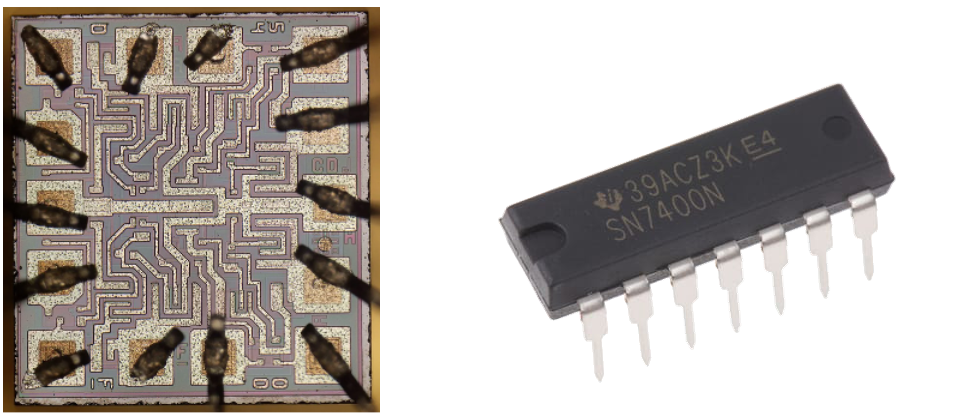
\includegraphics[width=0.40\textwidth]{lab-reports/Schematics-and-graphics/SN7400N.png}
\caption{Fotografia del DIE e del \textit{package} plastico DIP \textit{(Dual Inline Package)} dell'integrato con 2 porte NAND SN7400N}
\label{fig:integrated_nand}
\end{center}
\end{figure}

\subsection{Transistor di interfaccia PN2222A}
Gli integrati logici appena descritti, appartenendo alla famiglia TTL con stato alto a 5V, non possono essere collegati direttamente all'uscita degli amplificatori operazionali presenti nello stadio analogico del SAR, che operano tra +15V e -15V, si rende quindi necessaria l'introduzione di un transistor di interfaccia come il PN2222A, un BJT NPN \textit{general purpose} con $h_{fe}$ compreso tra 100 e 300 che tollera correnti di collettore fino a 600 mA. Questo dispositivo verrà utilizzato in configurazione ad emettitore comune in modalità interdizione / saturazione.
\cite{I}


\subsection{Integrato di \textit{sample holding} LF398}
Il convertitore SAR tratttato in questa relazione può campionare segnali variabili nel tempo sotto l'ipotesi di piccole variazioni di questi durante ciascun ciclo di campionamento e questo implica di utilizzare una frequenza di campionamento molto maggiore della frequenza delle armoniche di Fourier del segnale in ingresso. Per ottenere prestazioni migliori, raggiungendo il limite posto dal teorema di campionamento di Nyquist-Shannon, è necessario introdurre un circuito in grado di mantenere costante la tensione all'ingresso dell'ADC fino a quando il ciclo di conversione non viene completato. Questo viene realizzato mediante l'integrato monolitico \textit{sample and hold} LF398, che prevede un ingresso compatibile con la logica TTL per controllare la finestra di campionamento, due pin per il collegamento del condensatore che permetterà il mantenimento della tensione in uscita, due pin di alimentazione duale $\pm$ 15V e naturalmente i pin di ingresso e di uscita del segnale analogico. L'integrato necessita di meno di 10 $\mu s$ per effettuare il campionamento e il datasheet riporta una stabilità del guadagno pari allo 0.002 \%.
\cite{J}

\subsection{Scheda a microcontrollore}
Nell'ultima fase dell'esperienza di laboratorio verrà realizzato un semplice sistema di registrazione dei valori acquisiti utilizzando un microcontrollore \textit{Atmel ATmega328P} basato sull'architettura Harvard RISC a 8 bit interfacciato con un lettore di schede microSD. Questo MCU viene impiegato con un oscillatore esterno al quarzo a 16 MHz per il clock, dispone di 32 KB di memoria ISP flash e nel nostro caso è installato su una scheda Arduino che ospita anche un secondo microcontrollore \textit{Atmel ATmega16u2} con funzione di interfaccia di programmazione USB. La funzione di questo dispositivo è quella di leggere lo stato delle uscite dei J-K, corrispondente alla rappresentazione binaria del segnale campionato, e di scrivere i codici su un file salvato su una scheda microSD a cui è connesso mediante una linea seriale SPI.

%%%%%%%%%%%%%%%%%%%%%%%%%%%%%%%%%%%%%%%%%%%%%%%%%%%%%%%%

\section{Caratterizzazione dei circuiti logici fondamentali}
Si verificheranno rapidamente in laboratorio alcune caratteristiche significative di alcuni circuiti logici fondamentali, alcuni verranno utilizzati successivamente per la realizzazione dell'ADC.

\subsection{Verifica della tabella di verità della porta AND}
Una porta AND è un gate logico con due o più ingressi e un'uscita che esegue l'operazione di congiunzione logica. L'output di tale componente rispetta, infatti, la seguente tabella di verità:
\begin{center}
\begin{tabular}{ |c|c|c| } 
 \hline
 \rowcolor{lightgray}
 A & B & OUT \\ \hline \hline
 0 & 0 & 0 \\ \hline
 1 & 0 & 0 \\ \hline
 0 & 0 & 0 \\ \hline
 1 & 1 & 1 \\ \hline
\end{tabular}
\end{center}
In laboratorio utilizzando l'integrato \textbf{SN74LS08N} e fornendo in ingresso due onde quadre di frequenza 5 Hz oscillanti tra 0 e 5 V e sfasate di un quarto di periodo si è ottenuto il grafico in  \textit{figura \ref{fig:AND-table}} 
\begin{figure}[H]%[!ht]
\begin{center}
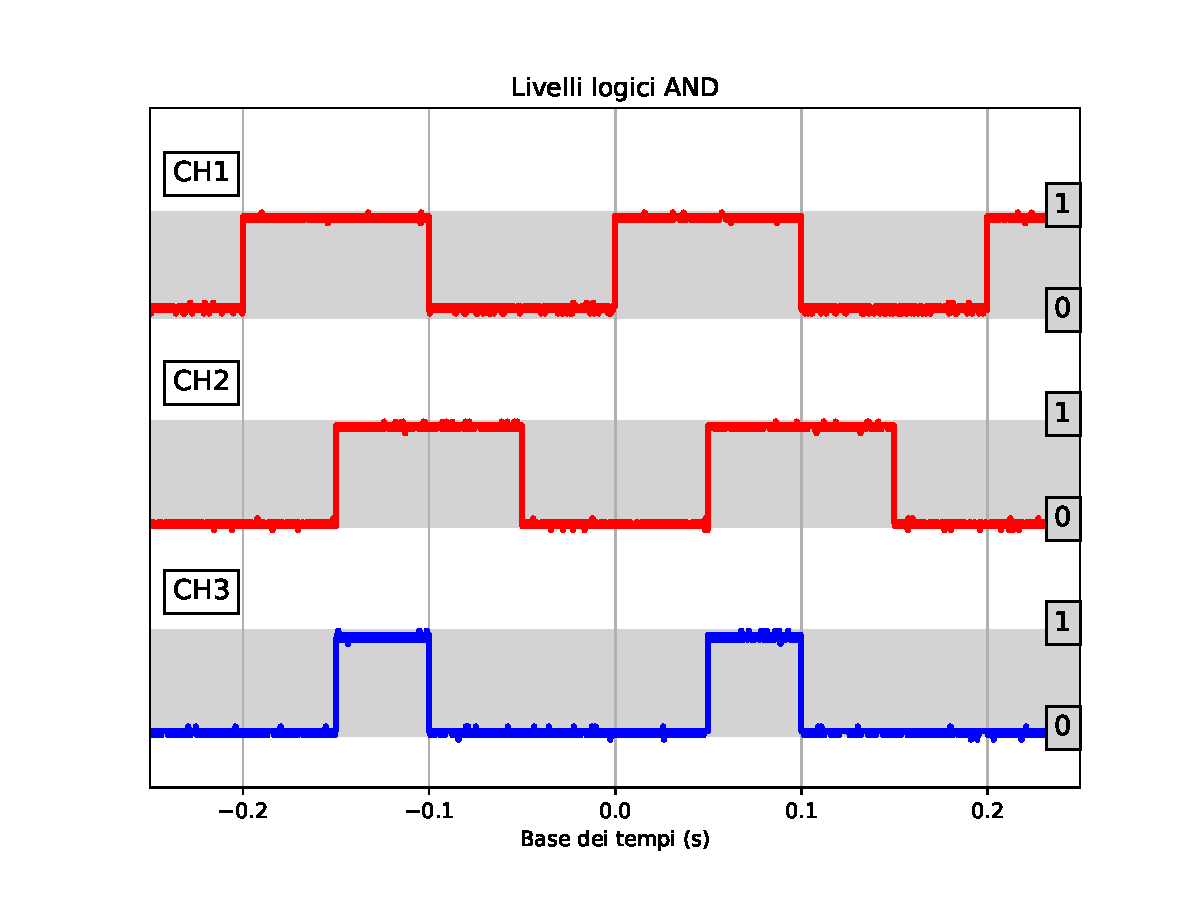
\includegraphics[width=0.50\textwidth]{analysis/output/AND-all.pdf}
\caption{Verifica della tabella di verità della porta logica AND}
\label{fig:AND-table}
\end{center}
\end{figure}

Lo sfasamento introdotto fa sì che si verifichino tutte le possibili combinazioni di stati logici agli ingressi A e B, permettendo la verifica dell'intera tabella di verità. Si osserva, in particolare, che l'uscita è allo stato alto solo quando lo sono sia A che B.

\subsection{Studio della caratteristica di trasferimento della porta NOT}

\begin{figure}[H]%[!ht]
\begin{center}
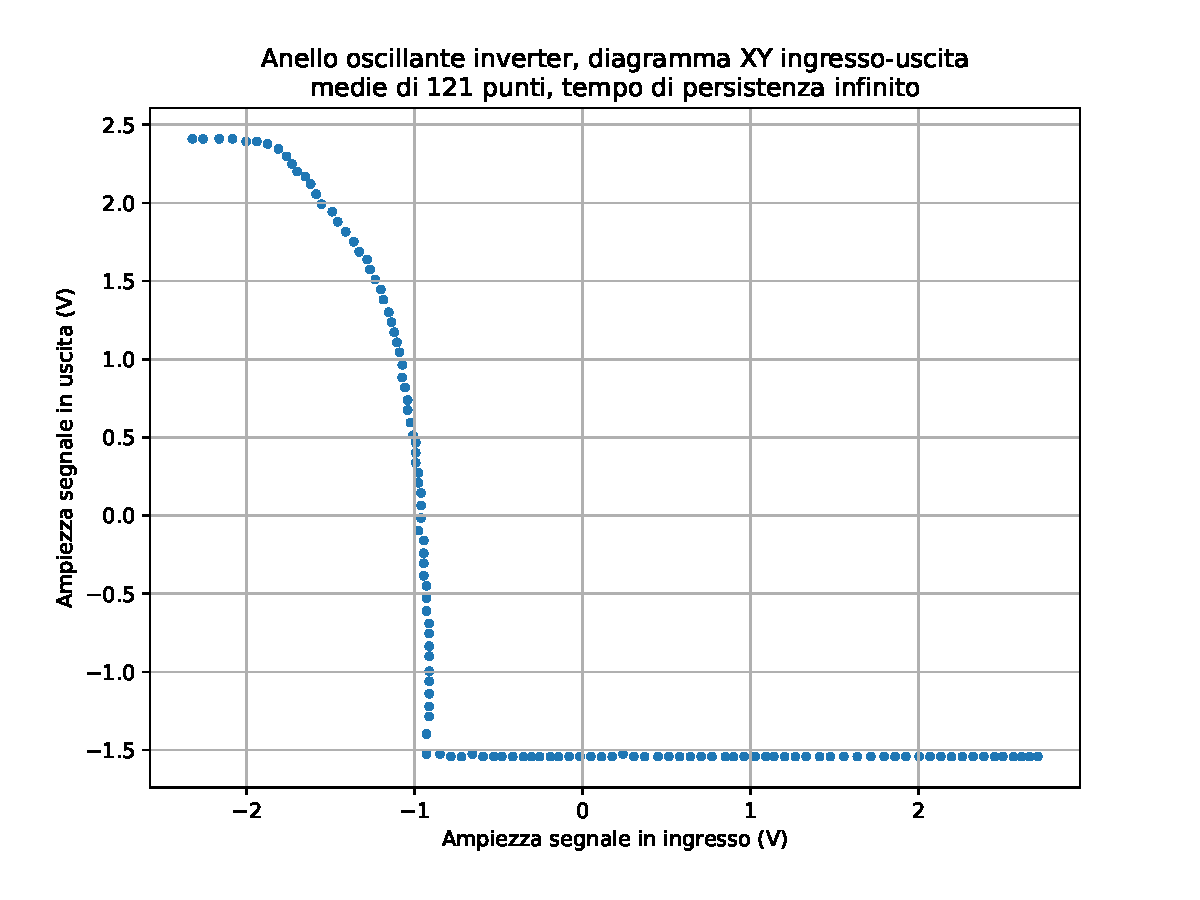
\includegraphics[width=0.45\textwidth]{analysis/output/inverter_ring_xy.pdf}
\caption{Caratteristica di trasferimento della porta NOT}
\label{fig:transf_not}
\end{center}
\end{figure}

Passiamo ora allo studio della caratteristica di trasferimento della porta NOT, rappresentata in \textit{figura \ref{fig:transf_not}}
, dove sull'asse orizzontale troviamo la tensione in ingresso e sull'asse verticale la tensione in uscita. La forma del fronte di discesa che distingue il livello di uscita alto dal livello di uscita basso è di fondamentale importanza per il buon funzionamento della porta logica, perché consente una progressiva rigenerazione di un segnale logico attenuato o affetto da rumore, man mano che esso attraversa più porte logiche, anziché un suo ulteriore degrado. Supponiamo infatti di avere un segnale logico basso (0 V) affetto da un rumore ampio 1 V che attraversa un buffer formato con due porte NOT in serie: dal grafico si osserva che la prima mapperà 1 V a 3.3 V circa, mentre la seconda mapperà 3.3 V precisamente a 0 V. Si è ottenuto così un effetto di reiezione del rumore.


\subsection{Studio della caratteristica di trasferimento della porta NAND}
Ripetiamo ora la medesima analisi per la porta NAND fissando un ingresso al livello alto 5 V e collegando, come già fatto in precedenza, l'altro ingresso al generatore di segnali impostato per produrre una rampa da 0 V a 5 V a f = 500 Hz. La figura è prodotta dall'oscilloscopio in modalità di visualizzazione XY con il canale orizzontale collegato all'uscita del generatore e il canale verticale all'uscita della porta NAND. Osserviamo una zona particolarmente rumorosa nell'intorno della tensione a cui la porta NAND effettua la commutazione e osserviamo che anche con l'uscita scollegata da qualsiasi carico la porta NAND non raggiunge i 5 V in uscita previsti dallo standard TTL, ciò nonostante, la posizione della soglia di commutazione a circa 1 V garantisce la corretta interpretazione di segnali alti con tensione di 4 V.

\begin{figure}[H]%[!ht]
\begin{center}
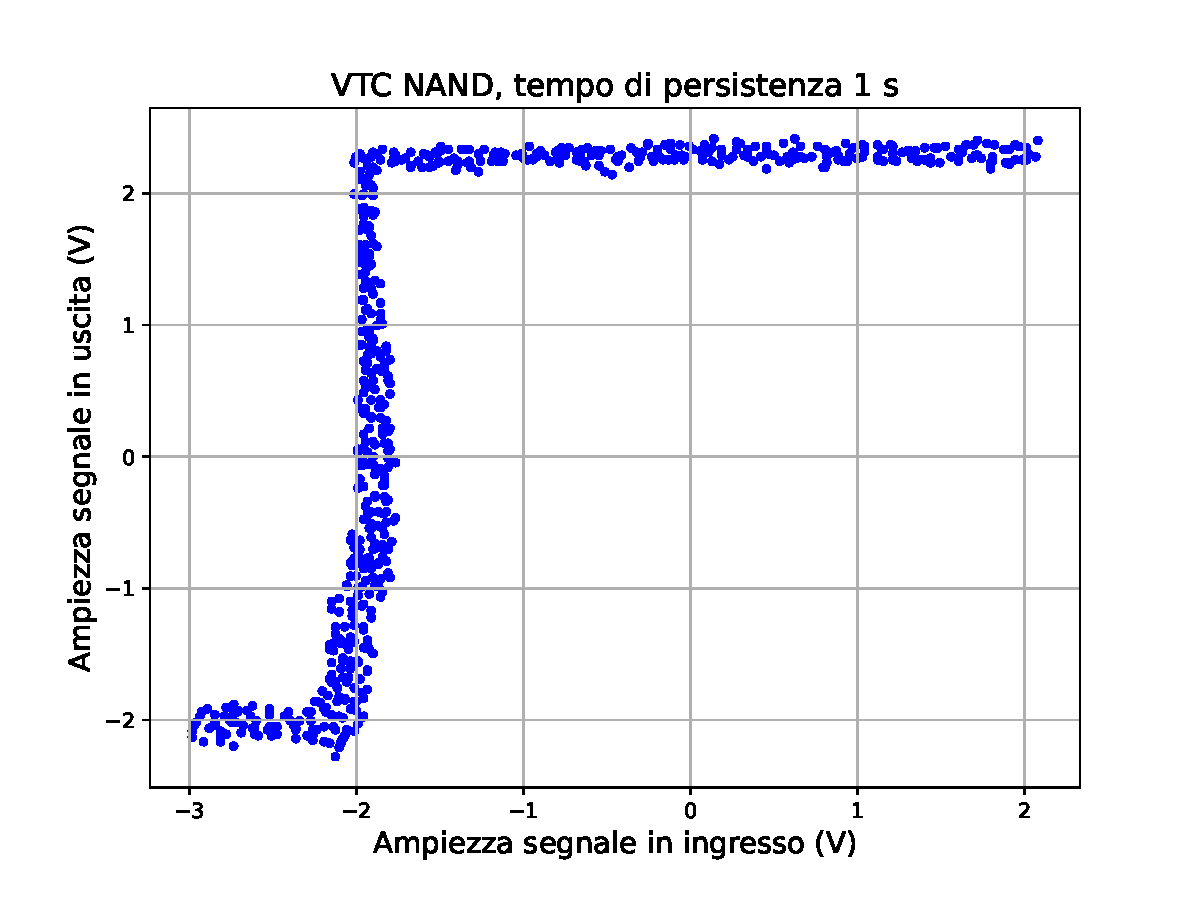
\includegraphics[width=0.45\textwidth]{analysis/output/NAND-XY.pdf}
\caption{Forma d'onda generata dal gate NAND}
\label{fig:VTC NAND gate}
\end{center}
\end{figure}


\subsection{Flip-flop di tipo set - reset}
\begin{figure}[H]%[!ht]
\begin{center}
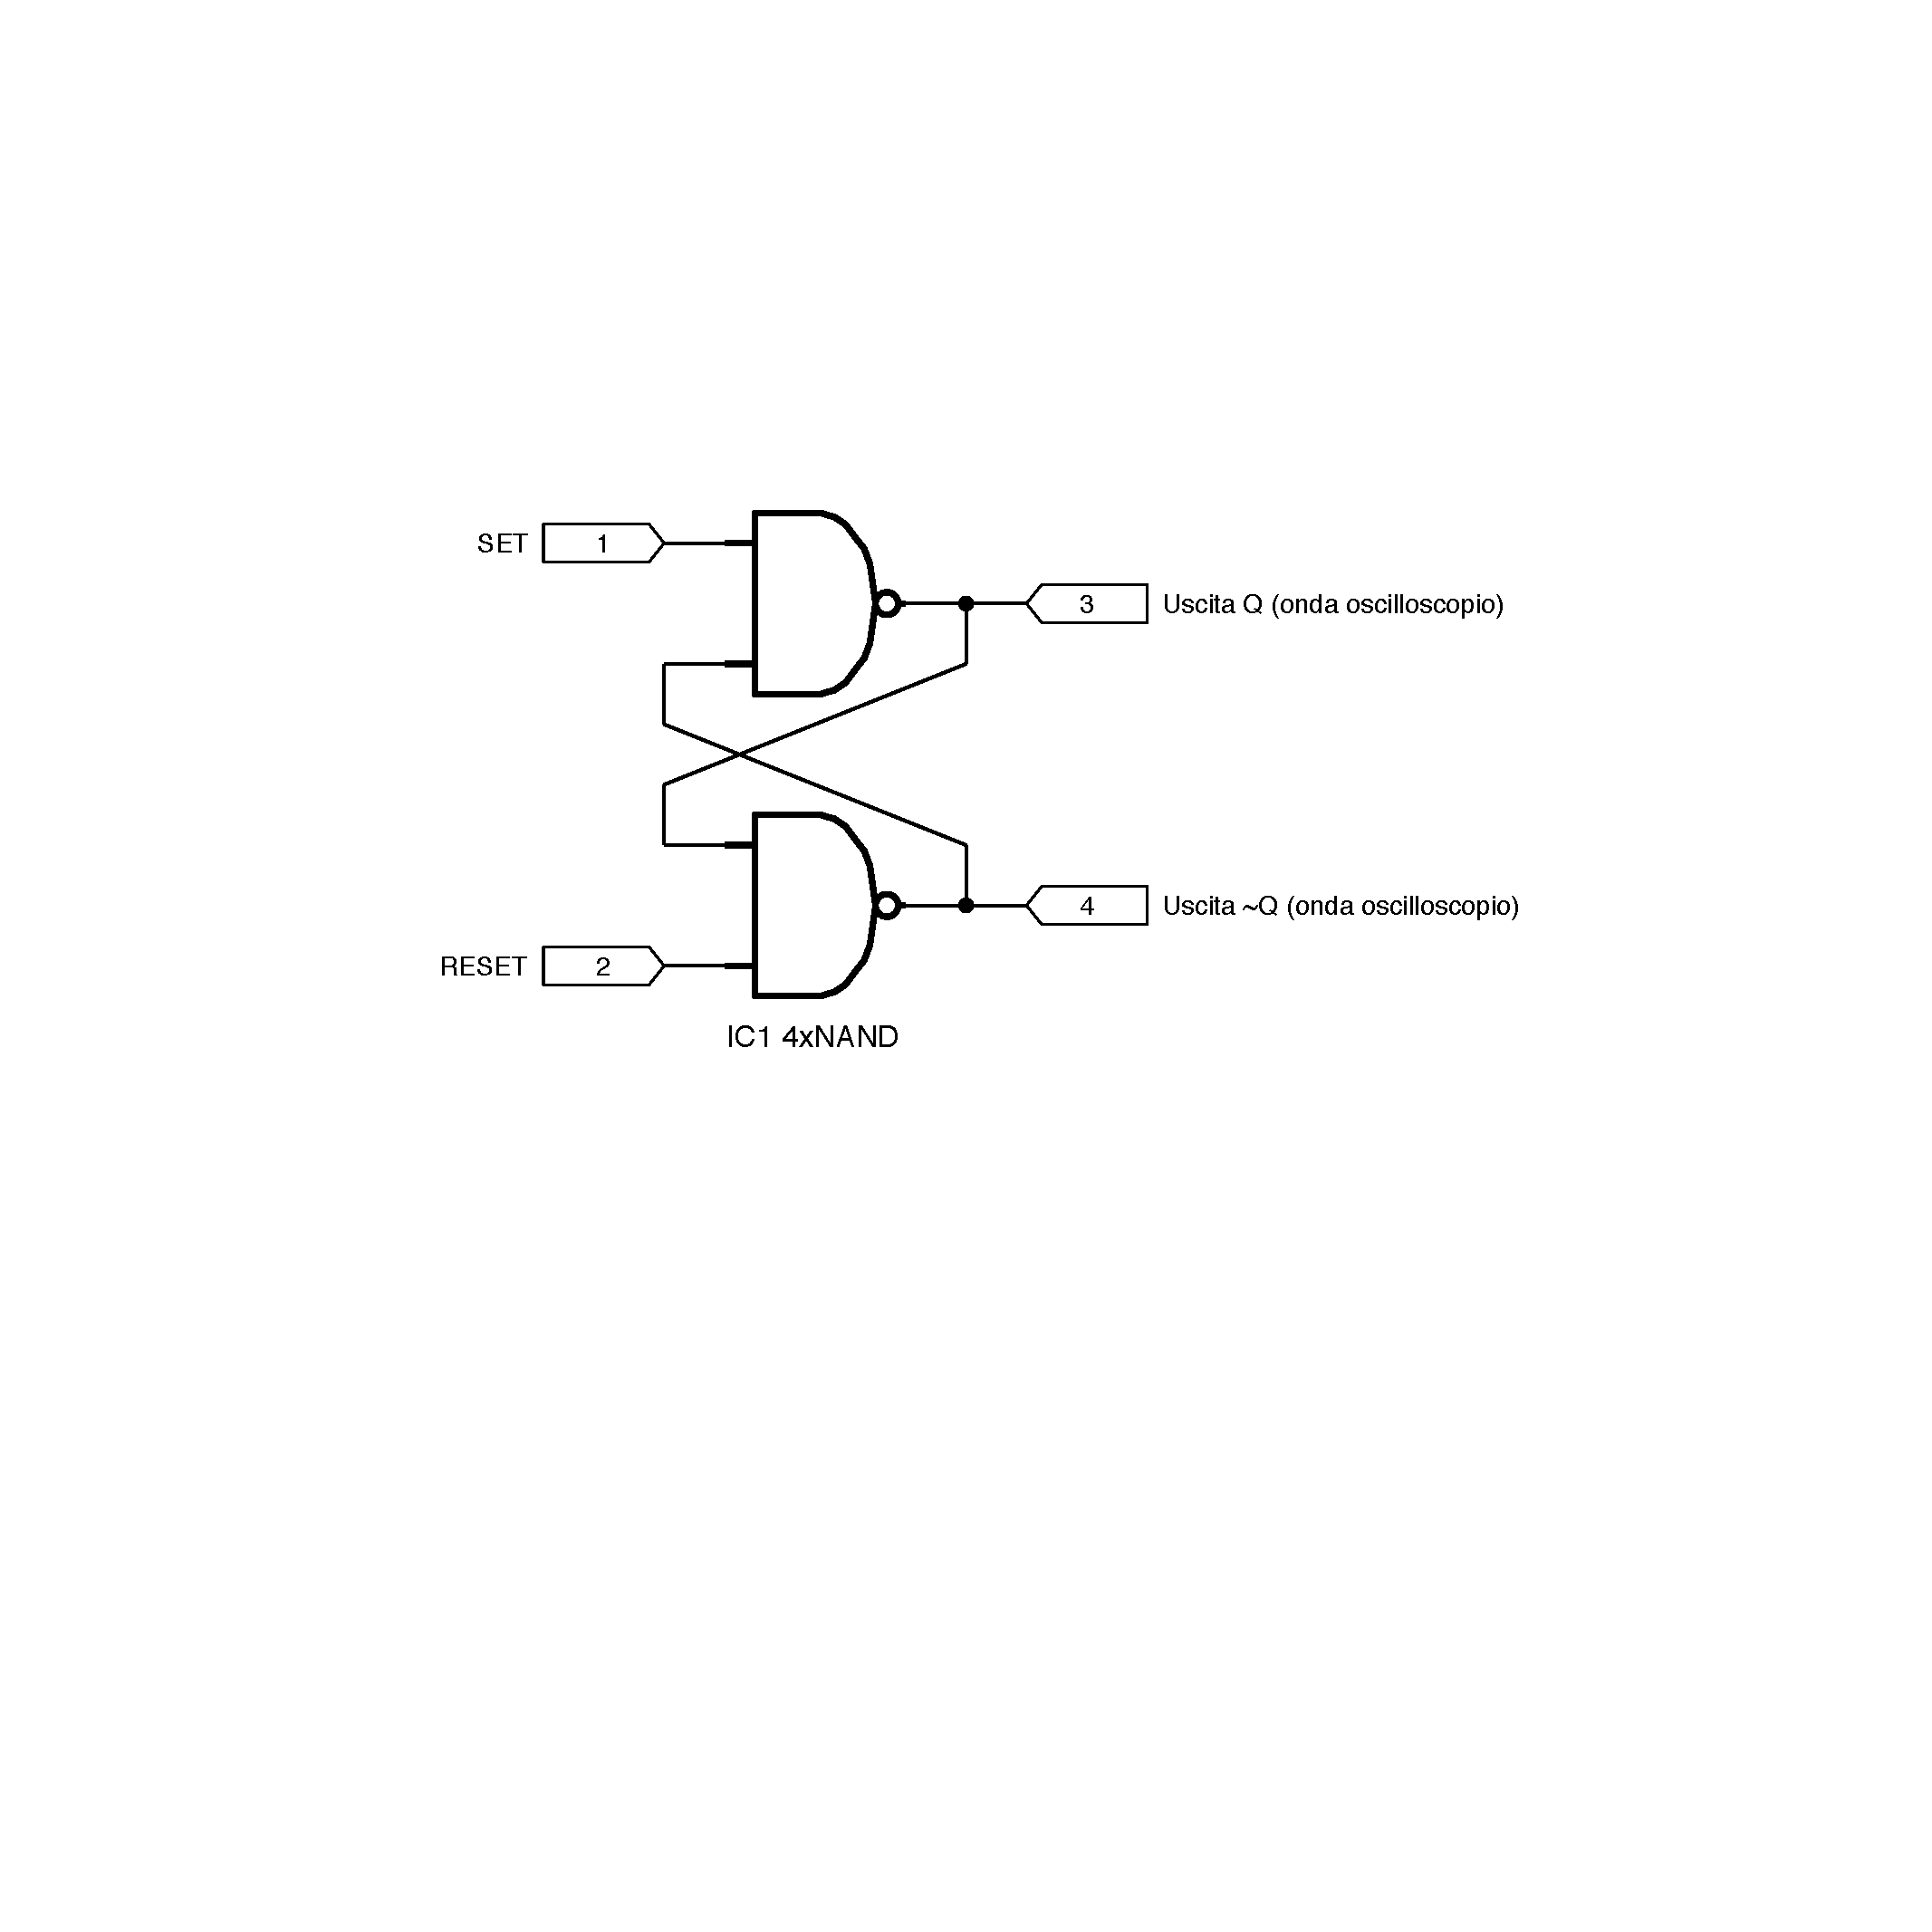
\includegraphics[width=0.30\textwidth]{sch-simulations/digital/output/flip-flop-RS.pdf}
\caption{Logica interna del flip-flop set-reset}
\label{fig:circuit_flip_flop}
\end{center}
\end{figure}
Il \textit{Flip-Flop SR }, noto  anche come \textit{SR latch}, è uno dei circuiti digitali sequenziali fondamentali, si tratta di un dispositivo di memoria bistabile a singolo bit. È dotato di due ingressi: \textit{SET} e \textit{RESET}. Quando entrambi si trovano ad 1 il flip flop si trova in stato di memoria, cioè lo stato delle uscite Q e $ \overline{Q}$ viene mantenuto costante, mentre quando uno tra gli ingressi SET e RESET viene portato a 0 l'uscita Q passa rispettivamente allo stato 1 o allo stato 0.
Il comportamento di un SR NAND Flip-Flop è quindi regolato dalla seguente tavola di verità:
\begin{center}
\begin{tabular}{ |c|c|c|c|c| } 
 \hline
 \rowcolor{lightgray}
S & R & Q & $\overline{Q}$ &\\ \hline \hline
 0 & 0 & 1 & 1 & Impredicibile\\  \hline
 0 & 1 & 1 & 0 & Stato stabile\\ \hline
 1 & 0 & 0 & 1 & Stato stabile\\ \hline
 1 & 1 & 0 & 1 & Memoria\\ \hline
 1 & 1 & 1 & 0 & Memoria\\ \hline
 
 \hline
\end{tabular}
\end{center}

In laboratorio è stato implementato un flip-flop RS utilizzando due porte logiche NAND dell'integrato \textit{SN74LS00N} e si è potuta verificare la tabella di verità osservando i segnali misurati con l'oscilloscopio mostrati nelle figure seguenti.

\begin{figure}[H]%[!ht]
\begin{center}
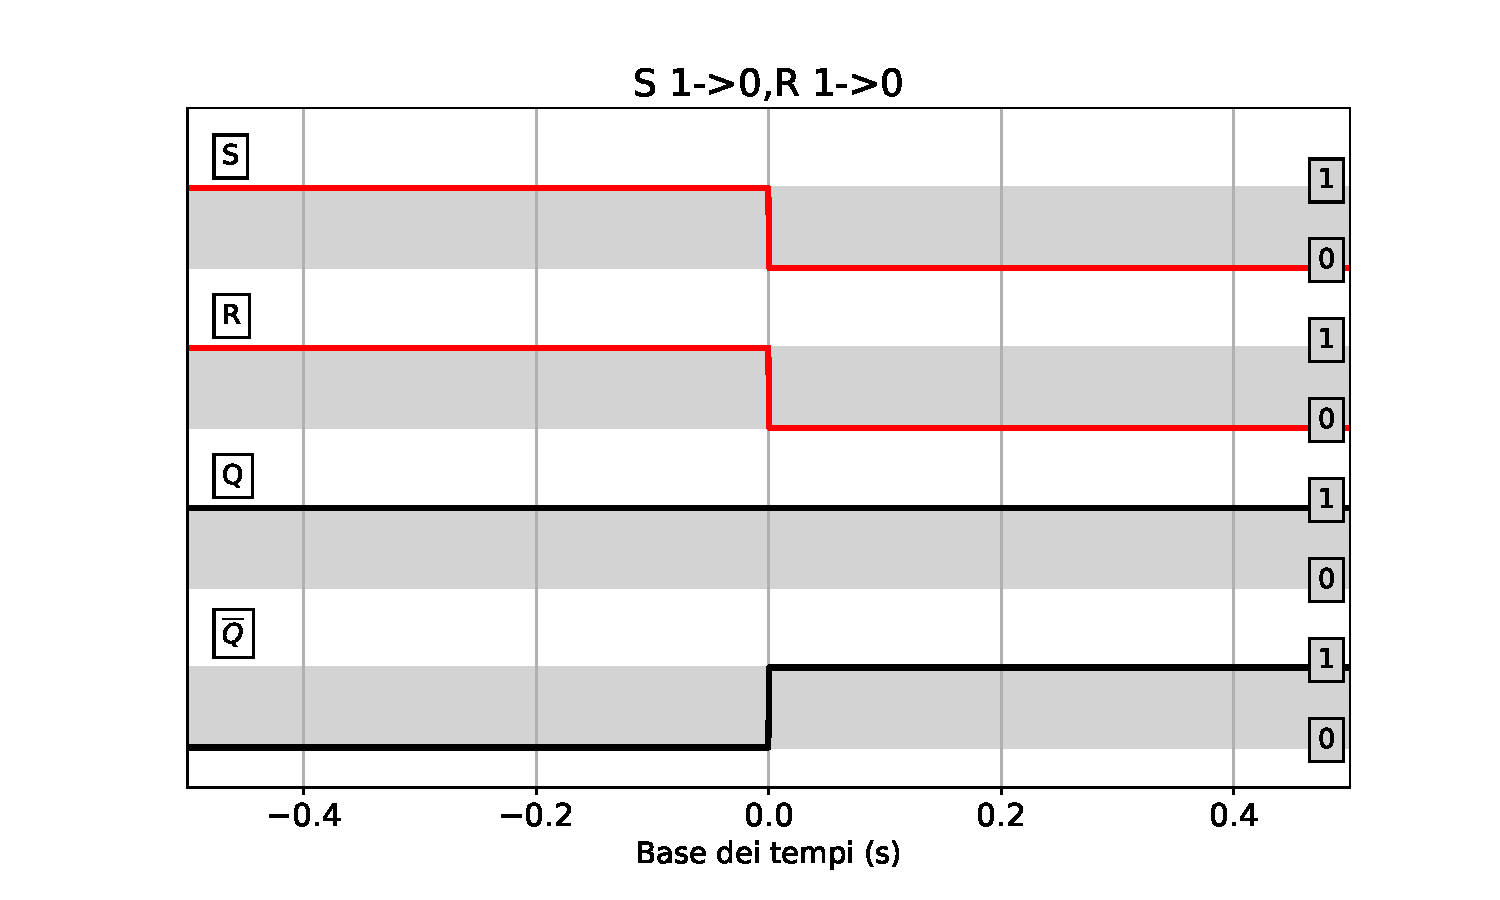
\includegraphics[ width=0.48\textwidth]{analysis/output/set-reset-to-0_0.pdf}
\label{fig:SR1}
\end{center}
\end{figure}

\begin{figure}[H]%[!ht]
\begin{center}
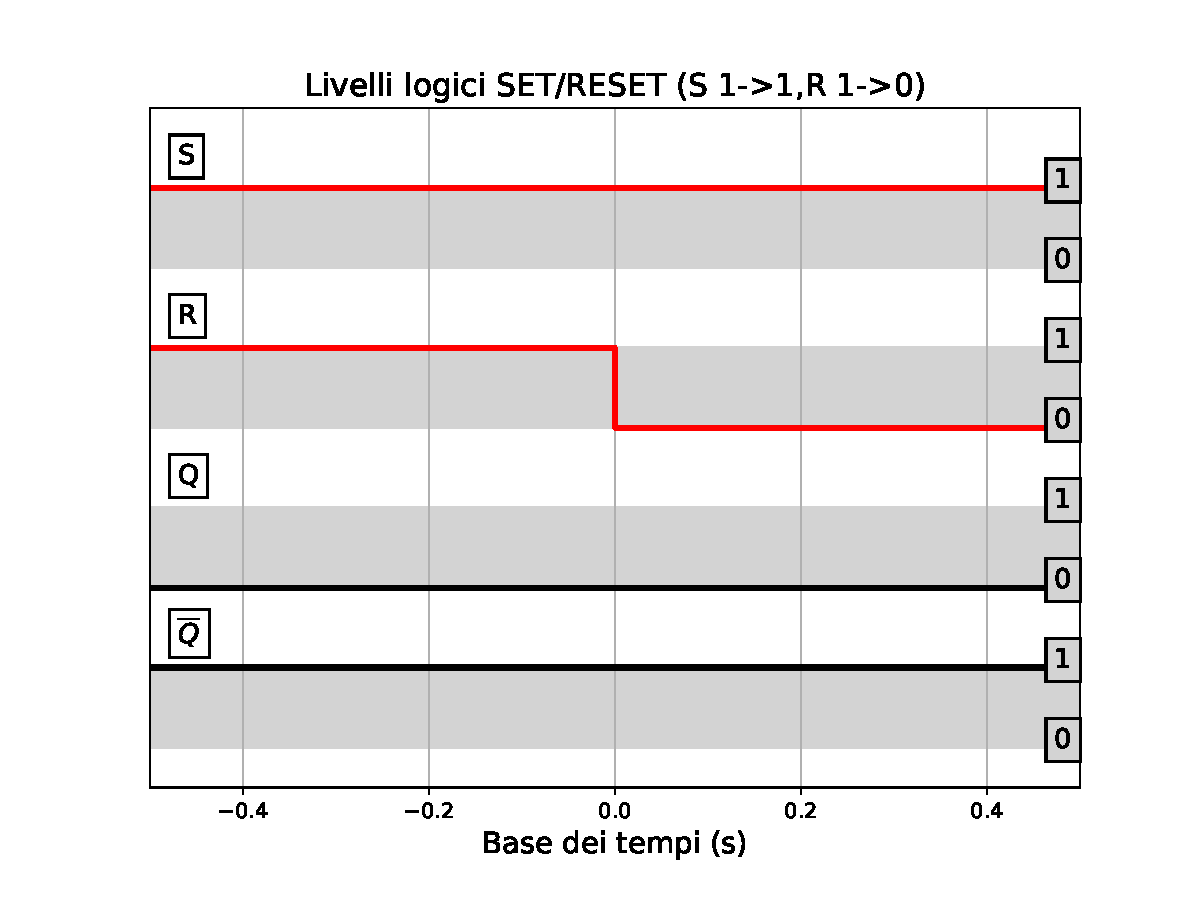
\includegraphics[ width=0.48\textwidth]{analysis/output/set-reset-to-1_0.pdf}
\label{fig:SR2}
\end{center}
\end{figure}

\begin{figure}[H]%[!ht]
\begin{center}
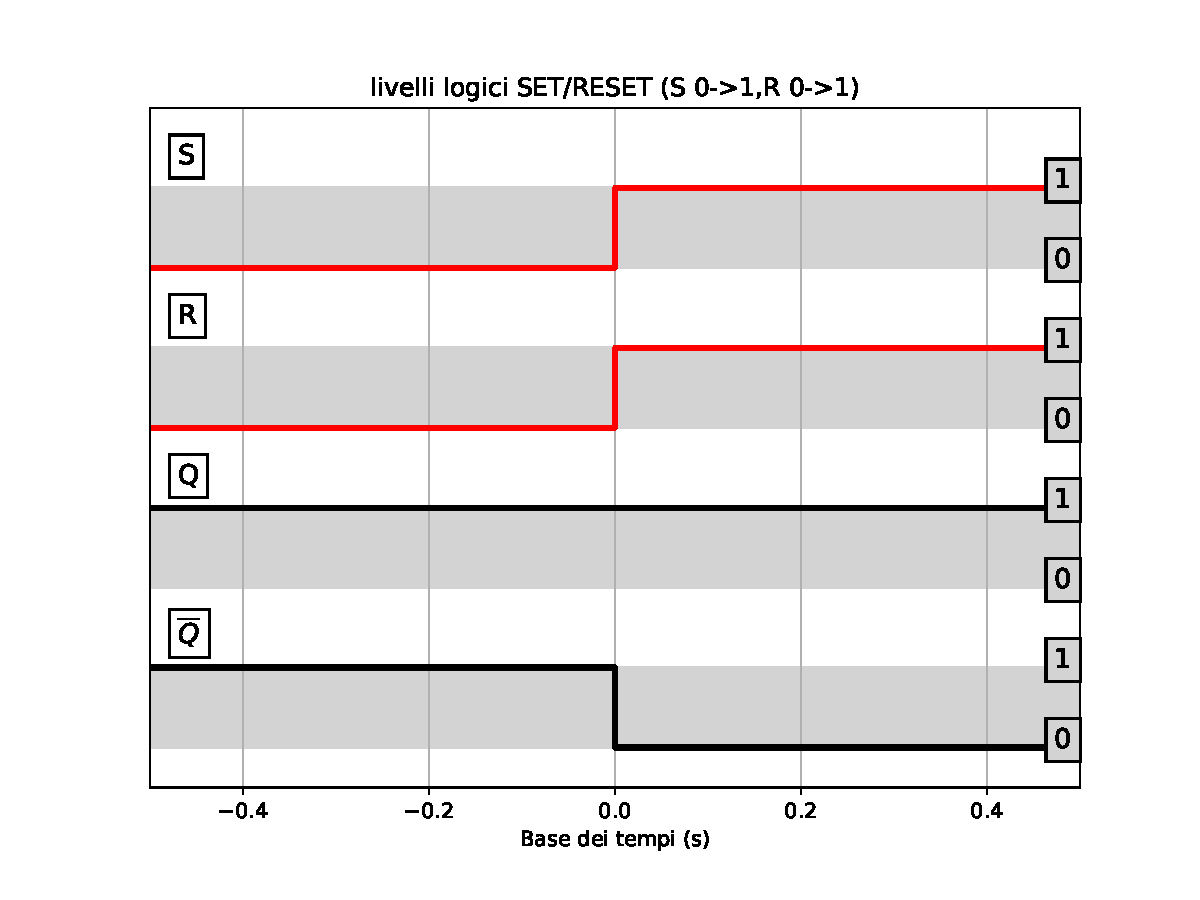
\includegraphics[ width=0.48\textwidth]{analysis/output/set-reset-to-1_1.pdf}
\label{fig:SR3}
\end{center}
\end{figure}

\begin{figure}[H]%[!ht]
\begin{center}
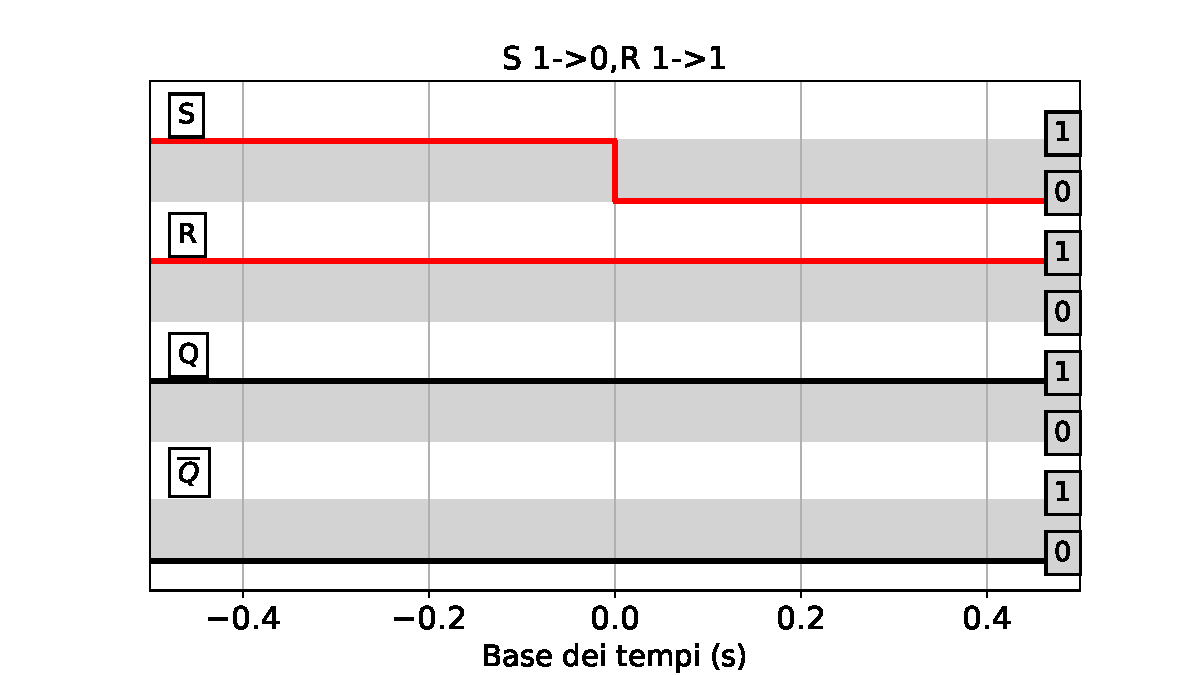
\includegraphics[ width=0.48\textwidth]{analysis/output/set-reset-to-0_1.pdf}
\caption{Verifica della tabella di verità di un flip-flop di tipo set-reset realizzato con porte NAND}
\label{fig:SR}
\end{center}
\end{figure}

%\begin{figure}[H]%[!ht]
%\begin{center}
%\includegraphics[trim = {0 0 580 0}, clip, %width=0.37\textwidth]{analysis/output/set-reset-table.pdf}
%porte NAND}
%\label{fig:SR-1}
%\end{center}
%\end{figure}


%\begin{figure}[H]%[!ht]
%\begin{center}
%\includegraphics[trim = {580 0 0 0}, clip, width=0.37\textwidth]{analysis/output/set-reset-table.pdf}
%\caption{Verifica della tabella di verità di un flip-flop di tipo set-reset realizzato con porte NAND}
%\label{fig:SR-2}
%\end{center}
%\end{figure}

Notiamo dalla \textit{figura \ref{fig:SR}} che il dispositivo si comporta nel modo atteso, verificando in ogni situazione i livelli logici predetti.
Questo dispositivo presenta però due limitazioni:
\begin{itemize}
    \item Lo stato con ingressi entrambi a 0 è impredicibile perché dipende dall'istante di tempo in cui il primo passa al valore basso e questo dipende tipicamente dal rumore; questo stato non viene praticamente mai utilizzato.
    \item L'operazione di latching avviene in modo asincrono, cioè appena uno degli ingressi si porta allo stato basso, non è previsto un ingresso di \textit{clock} che controlla l'istante di commutazione.
\end{itemize}
\subsection{Verifica della tabella di verità del flip-flop di tipo J-K}

Il \textit{JK Flip-Flop} è uno dei  flip-flop più diffusi nei circuiti digitali. Presenta due input \textit{J} e \textit{K} con funzioni analoghe al SET e RESET del latch visto in precedenza; il flip flop JK è in grado di superare entrambe le limitazioni prima elencate per quest'ultimo. Si tratta, infatti, di un flip-flop SR dotato di porte NAND a tre ingressi (realizzate con transistor ad emettitore triplo), che permettono sia l'introduzione di un segnale di \textit{clock} l'aggiunta di due nuovi circuiti di feedback dalle uscite che eliminano lo stato impredicibile sostituendolo con l'operazione di \textit{toggle}. Vi sono quindi quattro combinazioni logiche possibili per gli ingressi, riportate nella tabella di verità sottostante.
\newline
\begin{center}
\begin{tabular}{ |c|c|c|c|c| } 
 \hline
 \rowcolor{lightgray}
 J & K & Q & $\overline{Q}$ & $ Q_{n + 1} $ \\ \hline \hline
 0 & 0 &  &  & $Q_n$ \\ \hline
 1 & 0 & 0 & 1 & 1 \\ \hline
 1 & 0 & 1 & 0 & 1\\ \hline
 0 & 1 & 0 & 1 & 0 \\ \hline
 0 & 1 & 1 & 0 & 0 \\ \hline
 1 & 1 &  & & $\overline{Q_n}$ \\ \hline
\end{tabular}
\end{center}

\begin{figure}[H]%[t]
\centering
\begin{center}
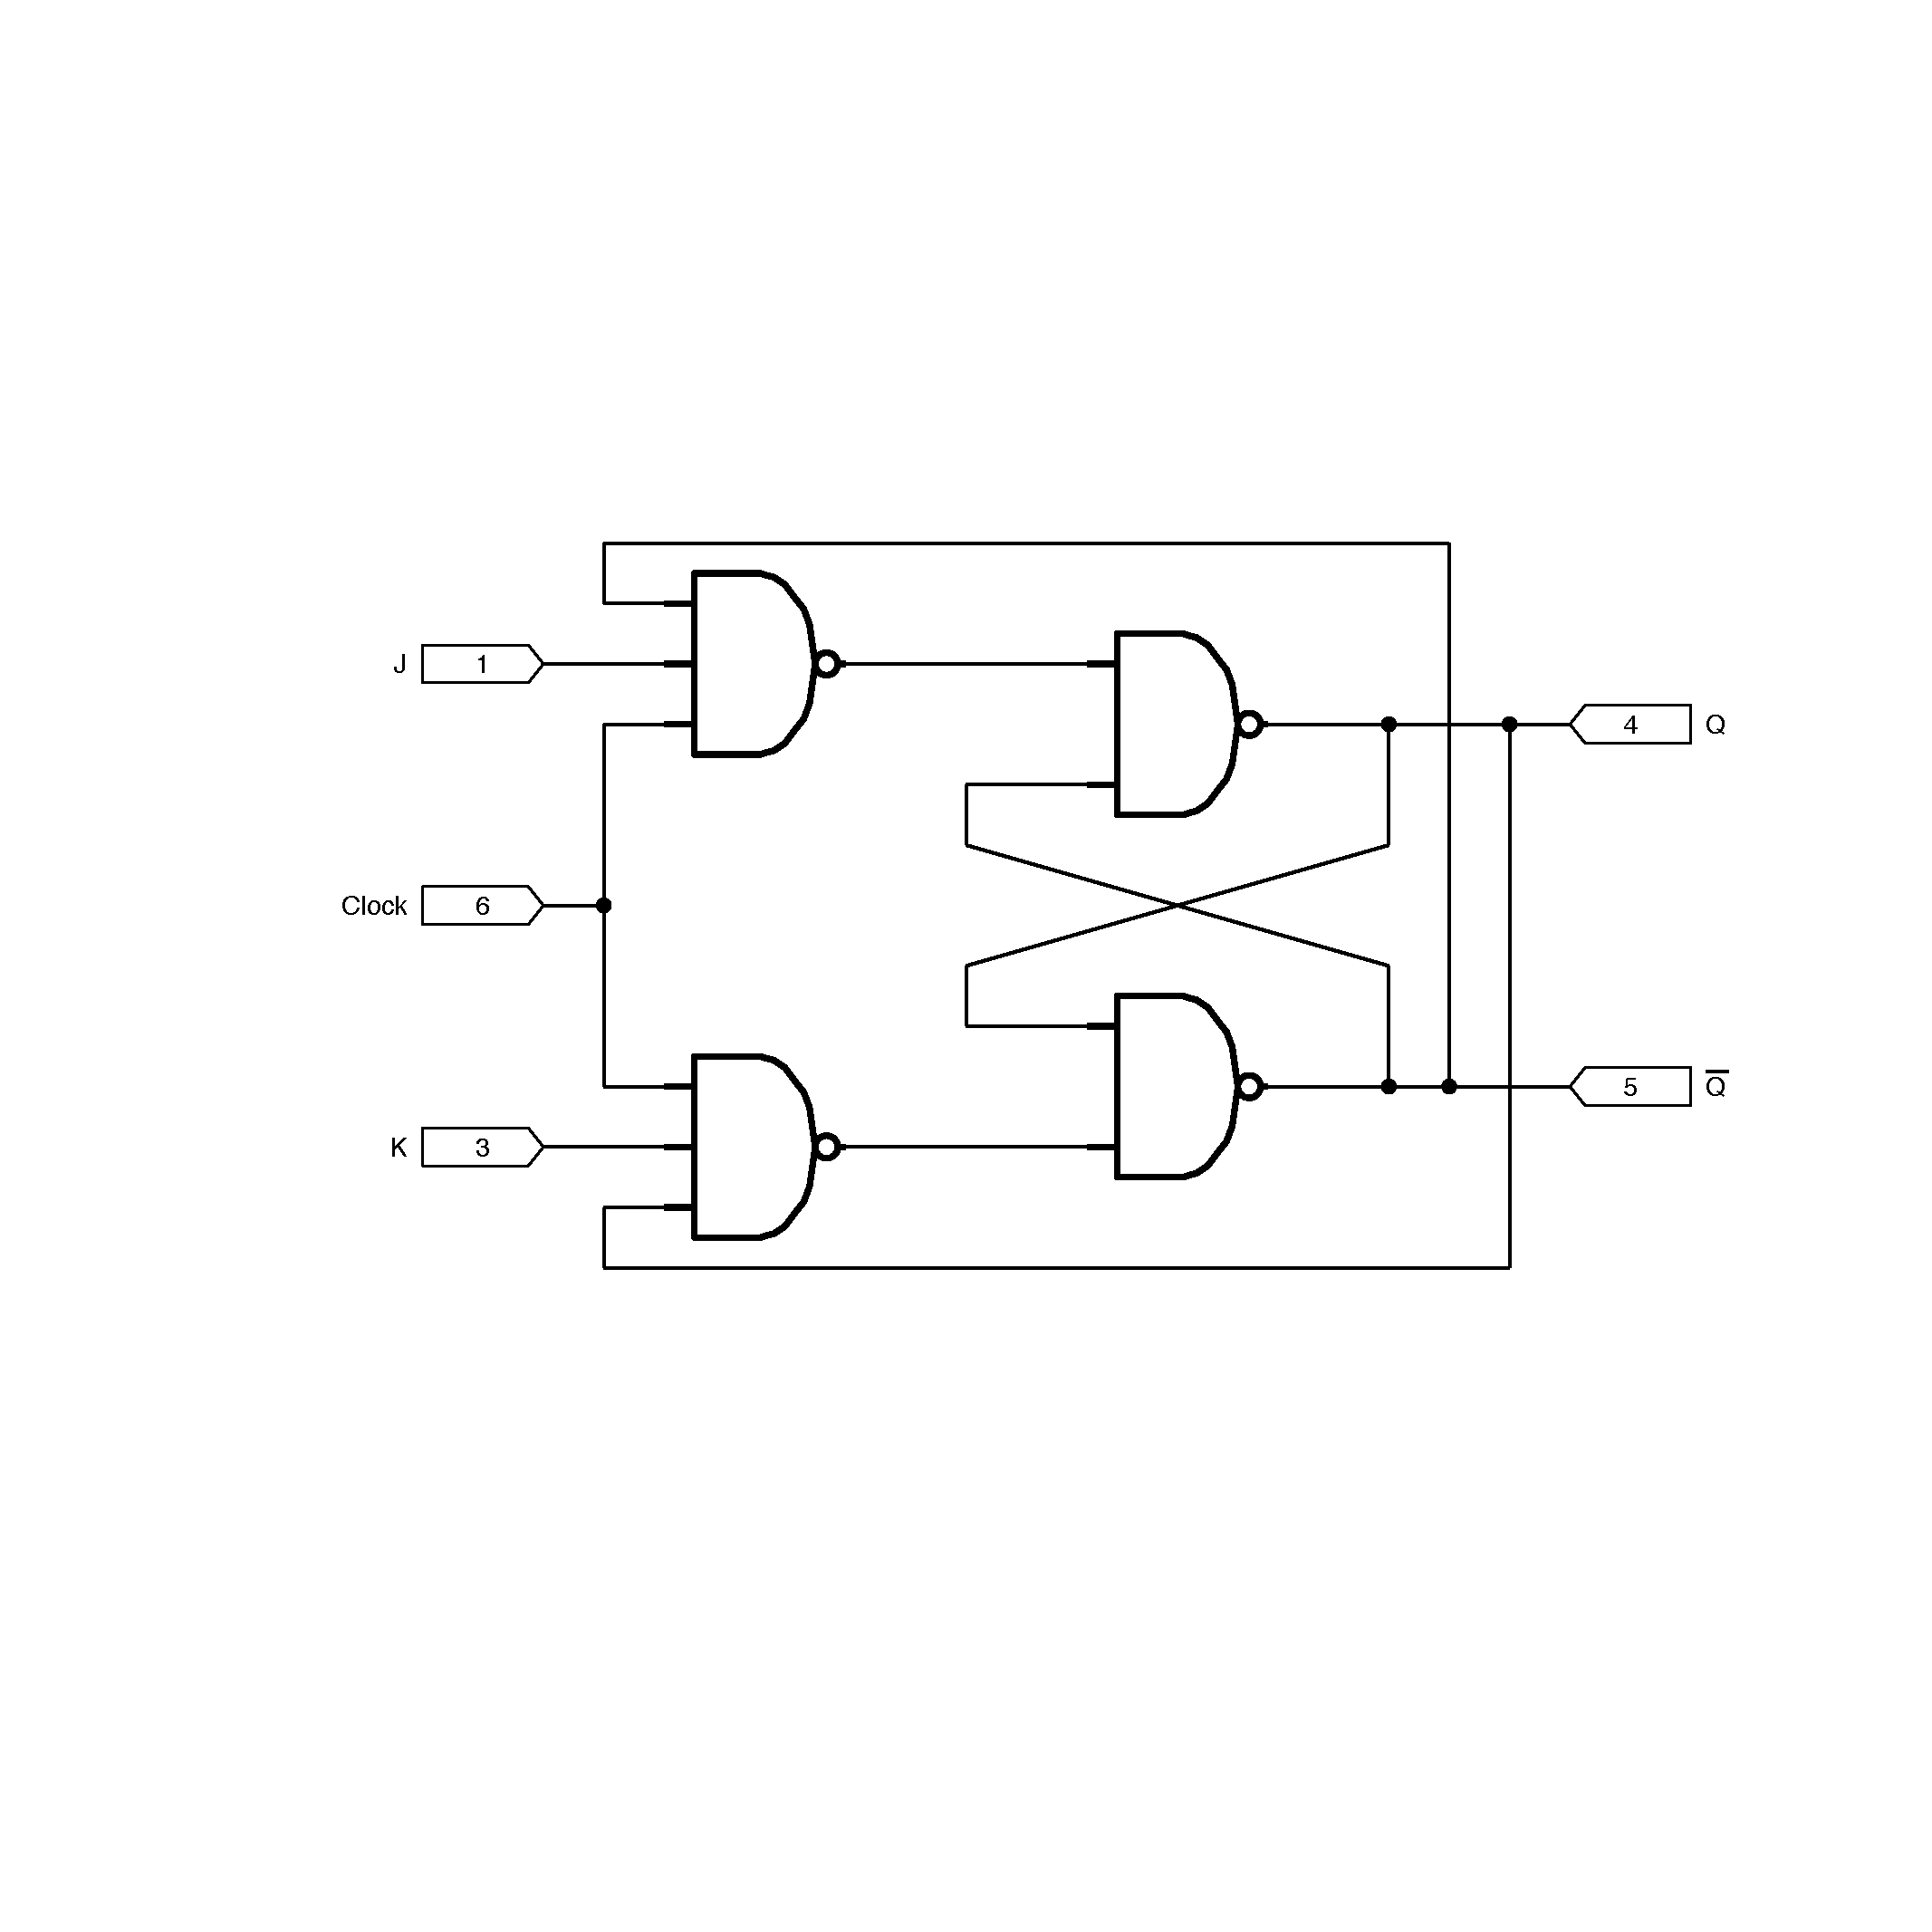
\includegraphics[width=0.40\textwidth]{sch-simulations/digital/output/flip-flop-JK.pdf}
\end{center}
\caption{Logica interna del flip-flop JK}
\label{fig:circuit_JK}
\end{figure}

\begin{figure*}[t]%[t]
\centering
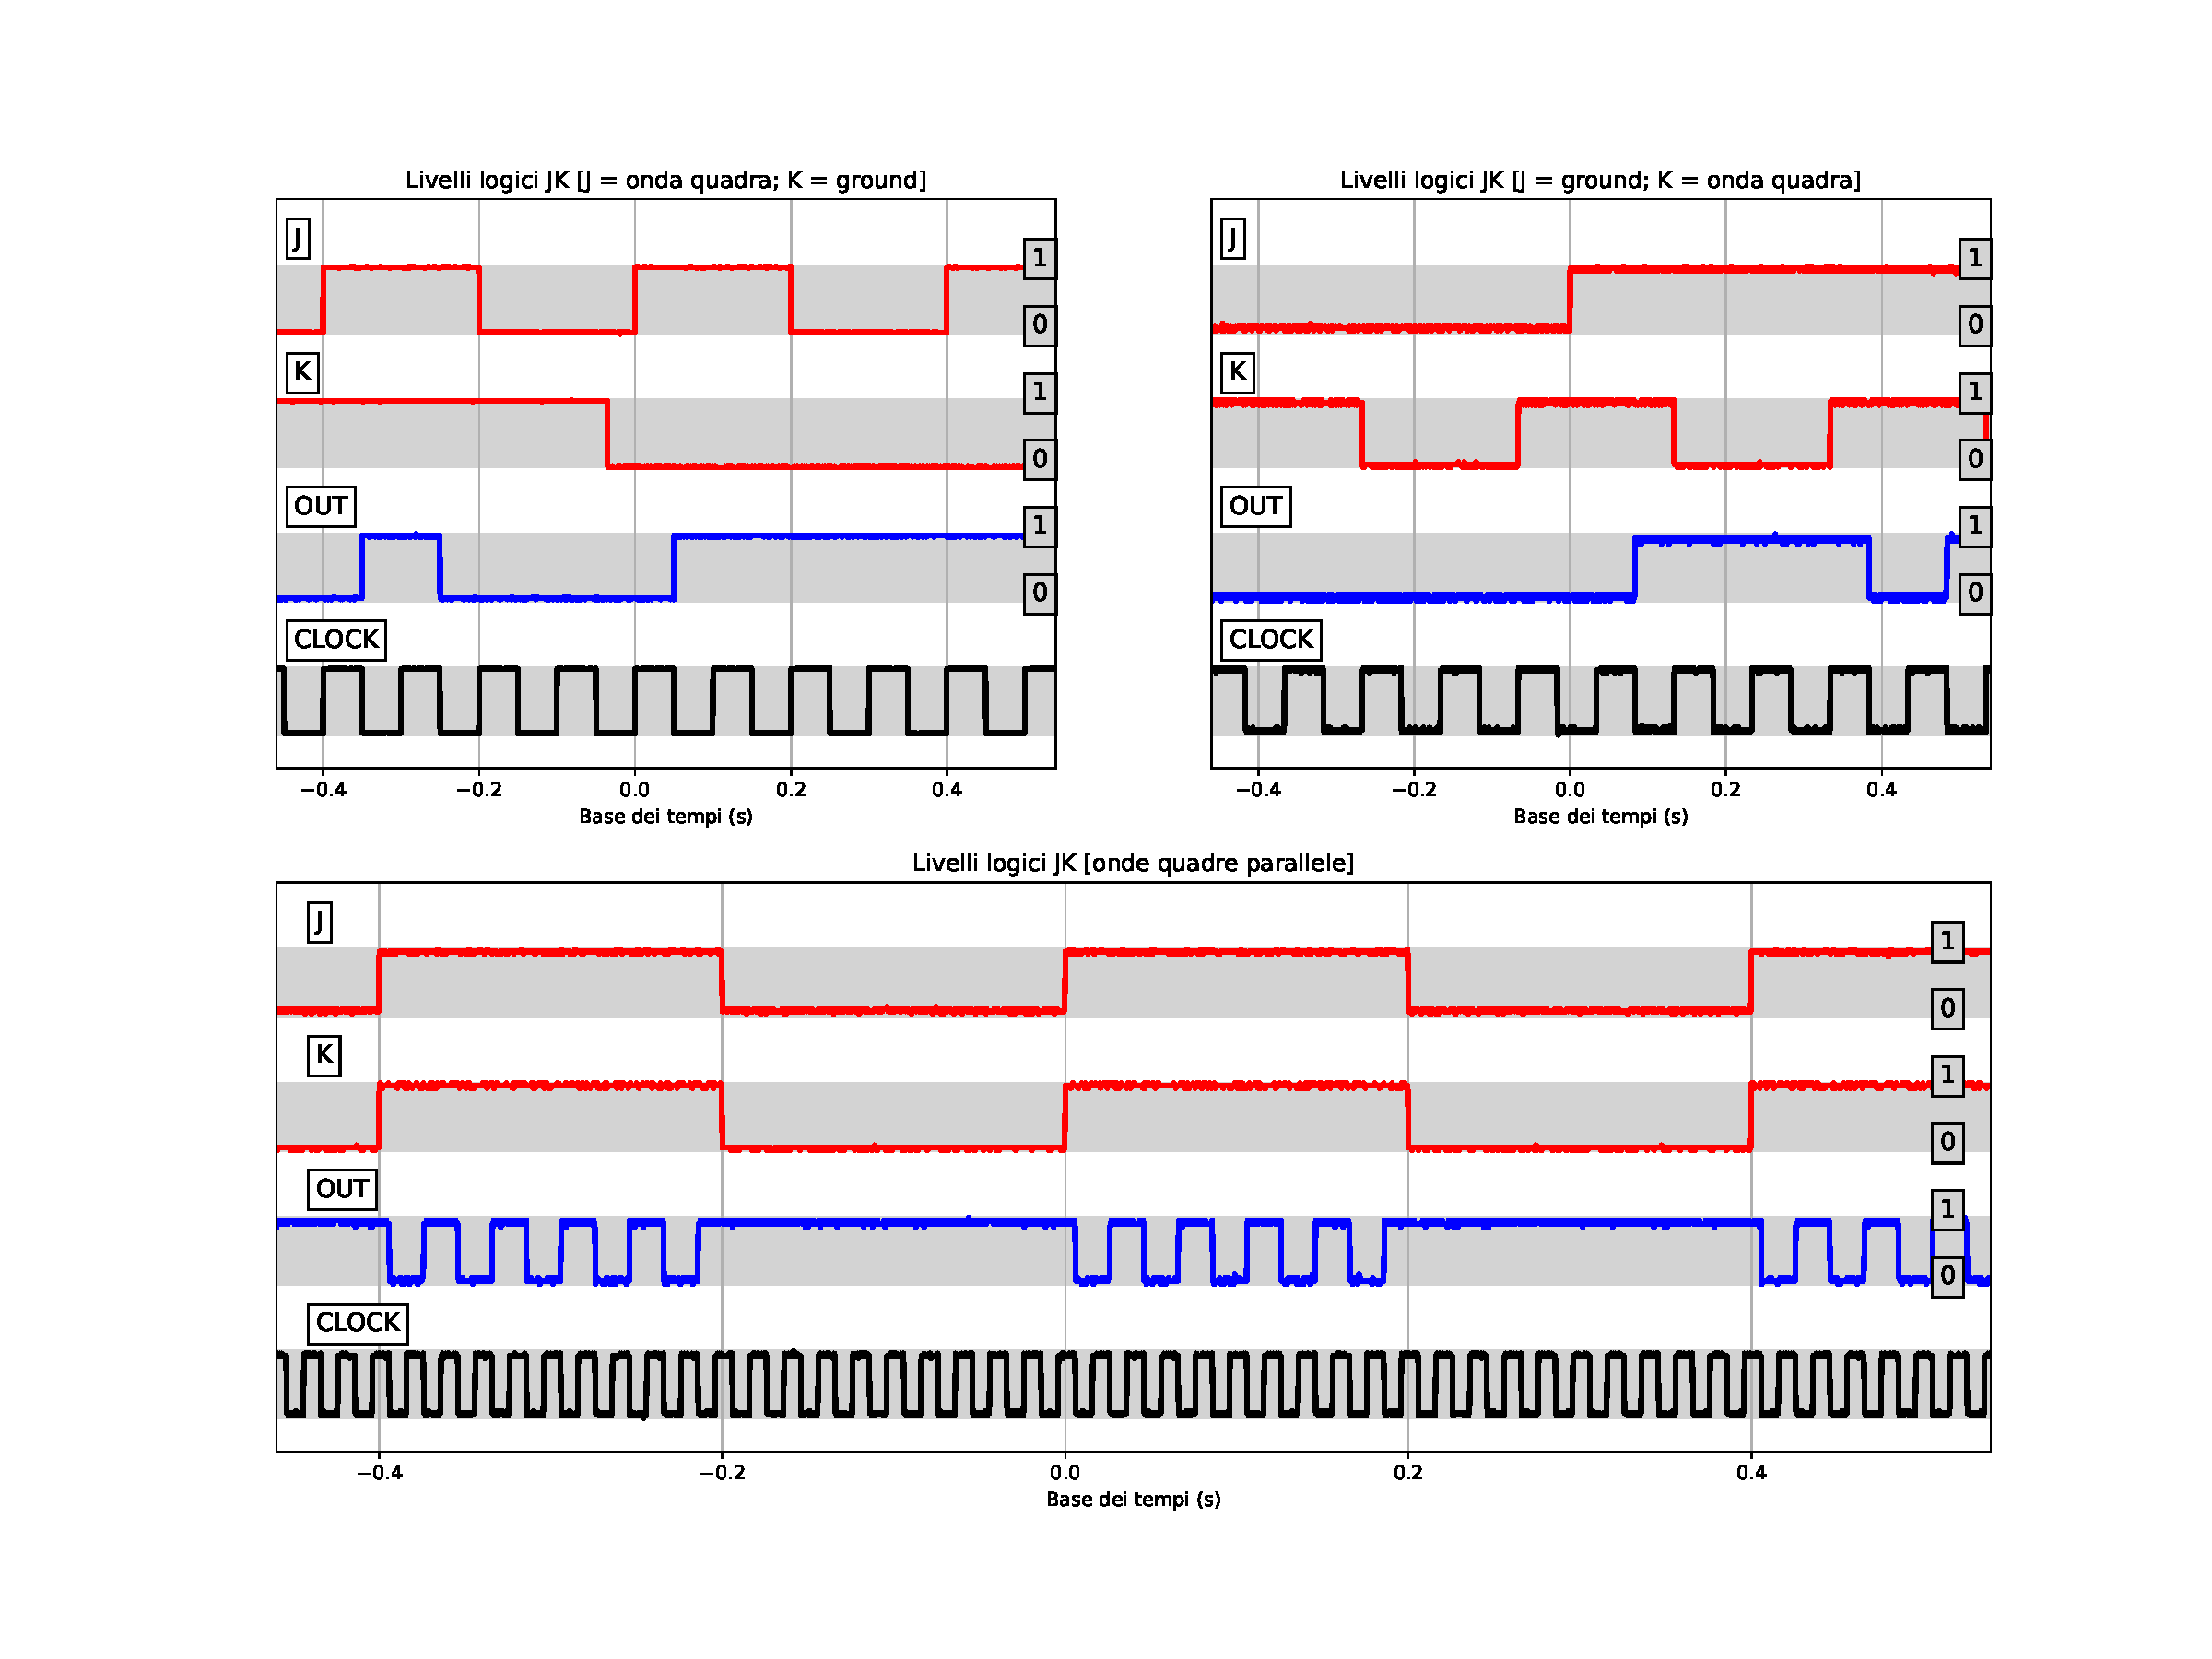
\includegraphics[width=0.95\textwidth]{analysis/output/JK-truth.pdf}
\caption{Verifica della tabella di verità di un flip-flop di tipo J-K}
\label{fig:jk-truth}
\end{figure*}
Discutiamo ora brevemente la verifica effettuata in laboratorio con l'integrato 74LS76AN.
Anche in questo caso il comportamento dell'integrato è quello atteso. Aspetti importanti da osservare sono in primo luogo il fatto che il cambio dei valori logici degli ingressi viene registrato nell'output solo dopo un fronte del \textit{clock} (nel nostro caso si tratta di un \textit{negative-edge flip-flop}) come ben evidente nei primi due grafici della \textit{figura \ref{fig:jk-truth}}. Per realizzare questa misura è stato collegato in modo alterno uno dei due ingressi ad un'uscita del generatore di segnali che produceva un'onda quadra, mentre l'altro ingresso era collegato ad un pulsante e controllava anche il trigger dell'oscilloscopio. 
Nel quadrante inferiore della figura osserviamo, invece, lo stato di \textit{toggle}, che si presente nel caso di J = K = 1, che noi abbiamo ottenuto collegando in parallelo i due ingressi ad un'uscita del generatore di segnali.
%%%%%%%%%%%%%%%%%%%%%%%%%%%%%%%%%%%%%%%%%%%%%%%%%%%%%%%%

\section{Verifica del funzionamento del ring oscillator realizzato con inverter}
Come anticipato nel paragrafo di descrizione degli integrati, il dispositivo SN74LS04 che implementa 6 porte NOT presenta un tempo di commutazione non trascurabile al variare del livello logico del segnale in ingresso alle alte frequenze e questo, se si realizza una catena di porte NOT, darà origine ad un ritardo di propagazione del segnale in ogni porta. 
Questo effetto porta a conseguenze interessanti se si realizza un anello chiuso con un numero dispari di inverter, nel nostro caso 7 suddivisi su due integrati. Si osserva infatti, collegando una sonda dell'oscilloscopio ad un punto arbitrario, che alimentando gli inverter le uscite cominciano ad oscillare liberamente con una forma d'onda che ricorda un'onda triangolare distorta con un periodo proporzionale al ritardo introdotto da ogni porta e al numero delle porte. Si sottolinea che il circuito risultante è un vero e proprio oscillatore, in quanto è in grado di produrre un'uscita periodica a partire da ingressi costanti nel tempo e non necessita di alcun innesco esterno se non quello dato dal rumore.

\begin{figure}[H]%[!ht]
\begin{center}
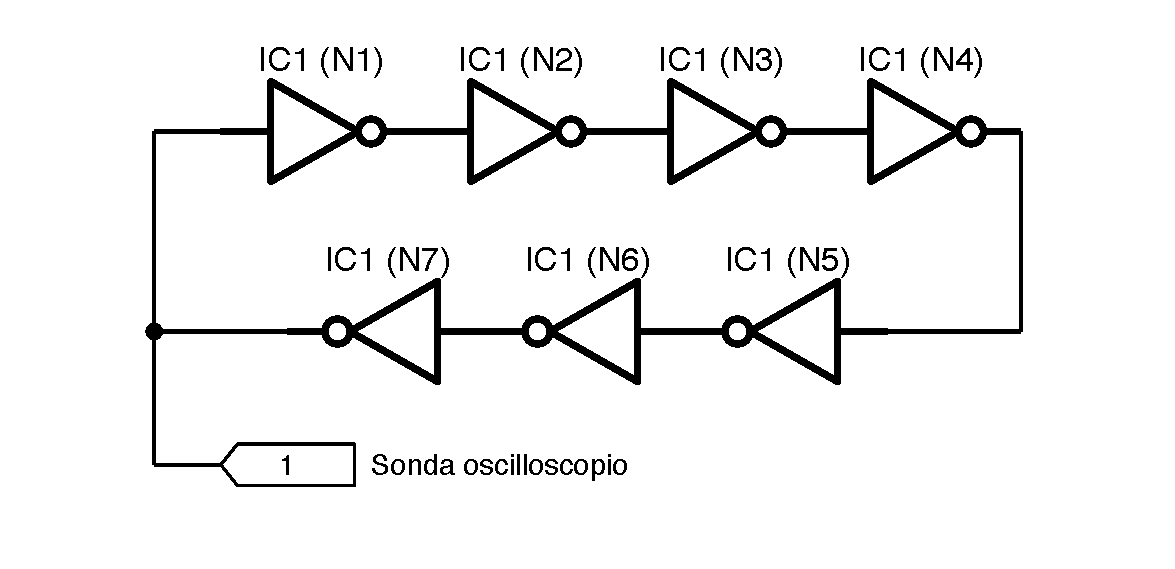
\includegraphics[width=0.40\textwidth]{sch-simulations/digital/output/ring-osc-logic.pdf}
\caption{Circuito equivalente dell'oscillatore ad anello}
\label{fig:circuit_ring_oscillator}
\end{center}
\end{figure}

Tra il ritardo di propagazione (t), il numero delle porte (n) e la frequenza della tensione oscillante generata (f) vale la presente relazione: 
\begin{math}
f = \frac{1}{2tn}
\end{math}
In laboratorio è stata acquisita la forma d'onda seguente, la cui frequenza risulta essere f = (12.66 $\pm$ 0.01) MHz, corrispondente ad un ritardo di propagazione medio tra gli inverter t = (5.6428 $\pm$ 0.0007) ns.


\begin{figure}[H]%[!ht]
\begin{center}
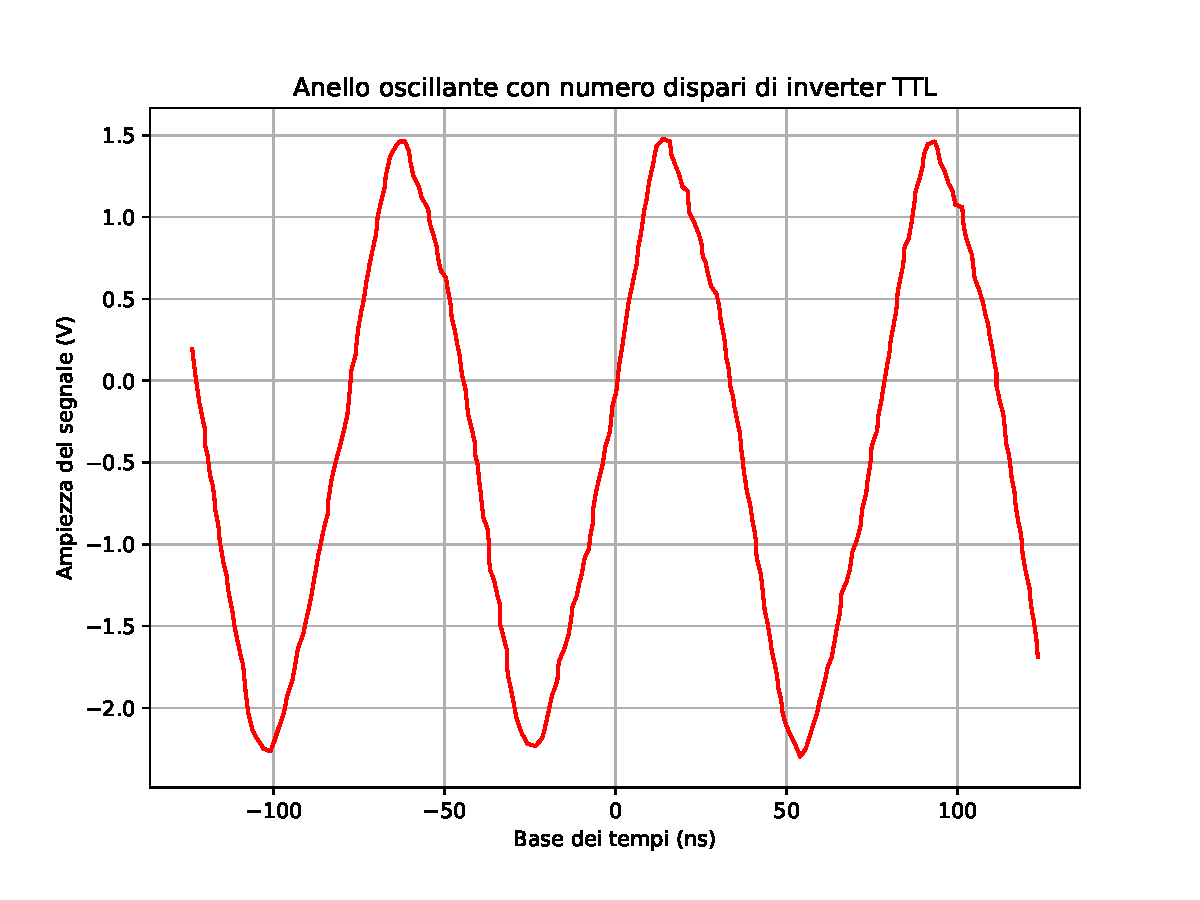
\includegraphics[width=0.50\textwidth]{analysis/output/oscillating-ring.pdf}
\caption{Forma d'onda generata dall'anello di inverter}
\label{fig:graph_ring_oscillator}
\end{center}
\end{figure}

Oscillatori di questo tipo sono utili per numerose applicazioni che spaziano dai VCO (voltage controller oscillators) dei phased-locked-loops (PLL) impiegati per generare il clock di tutte le moderne CPU fino alla generazione di numeri casuali sfruttando il jitter.

%%%%%%%%%%%%%%%%%%%%%%%%%%%%%%%%%%%%%%%%%%%%%%%%%%%%%%%%

\section{Realizzazione di un ADC SAR a 4 bit}

\subsection{Descrizione generale e specifiche tecniche desiderate}
Dopo aver preso in esame alcuni circuiti logici fondamentali, verrà ora affrontata la progettazione, calibrazione e verifica di un ADC ad approssimazioni successive (SAR) con risoluzione di 4 bit, rappresentato nello schema in figura \ref{fig:circuit_sarCompleteSchematic}. Questa tipologia di convertitori analogico - digitali è molto diffusa, sia in circuiti integrati stand alone (per esempio \textit{Analog Devices AD4695} sia all'interno di microcontrollori (per esempio la serie \textit{STM32} della \textit{ST Microelectronics}) e consente di raggiungere un buon compromesso tra frequenza di campionamento e risoluzione.

Il convertitore SAR che verrà realizzato utilizza un registro di scorrimento a 8 bit, pertanto la frequenza di campionamento sarà pari a un ottavo della frequenza di clock che durante la caratterizzazione è stata posta al massimo a 10 KHz. In questo regime di funzionamento il convertitore si è sempre mostrato affidabile, mentre a frequenze maggiori gli amplificatori operazionali dello stadio analogico costituiscono il collo di bottiglia del sistema. Il convertitore ha un tempo di acquisizione dato dalla lunghezza della finestra in cui l'integrato \textit{sample and hold} LF398 effettua il campionamento, pari a un periodo del clock.

Il convertitore si compone dei seguenti blocchi funzionali fondamentali (con riferimento allo schema in figura \ref{fig:circuit_sarCompleteSchematic}):
\begin{itemize}
    \item Un registro di scorrimento a 8 bit (U7) che permette di effettuare la scansione dei bit nel processo di confronto del segnale in ingresso ad approssimazioni successive, insieme a due circuiti di controllo implementati con porte NAND: il primo, basato su U8, genera il segnale di \textit{clear} che effettua il reset degli integrati TTL al termine del ciclo di conversione, mentre il secondo, basato su U9, inizializza l'ingresso del registro all'inizio di ogni ciclo di conversione.
    \item Una logica comprendente 4 porte AND implementate nell'integrato U5 che controllano 4 flip-flop di tipo J-K, implementati negli integrati U3 e U4. (MSB su U3). I flip-flop J-K vengono settati (J) in sequenza dalle uscite del registro di scorrimento e vengono resettati (K) quando viene settato il flip-flop successivo solamente se il circuito comparatore ha come complemento logico dell'uscita uno stato alto. Al termine di un ciclo del registro le uscite dei J-K rappresentano quindi il risultato della conversione.
    \item Uno stadio analogico che confronta il segnale in ingresso con la sua rappresentazione fornita dalle uscite dei J-K, composto da un DAC R-2R controllato da queste ultime la cui uscita viene confrontata mediante un OPA LM741 ad anello aperto (U2) con la tensione da campionare. L'uscita del comparatore pilota le porte AND che resettano i J-K mediante un transistor di interfaccia che garantisce sia la compatibilità dei livelli logici (l'uscita arriva a +15 V, mentre TTL prevede lo stato alto a +5 V), sia un più rapido fronte di commutazione. Lo stadio analogico può essere completato inserendo un circuito di \textit{sample and hold} a monte, pilotato dal registro a scorrimento.
    
\end{itemize}
 

\subsection{Verifica del circuito con registro di scorrimento e annessa logica di controllo}

\begin{figure}[H]%[!ht]
\begin{center}
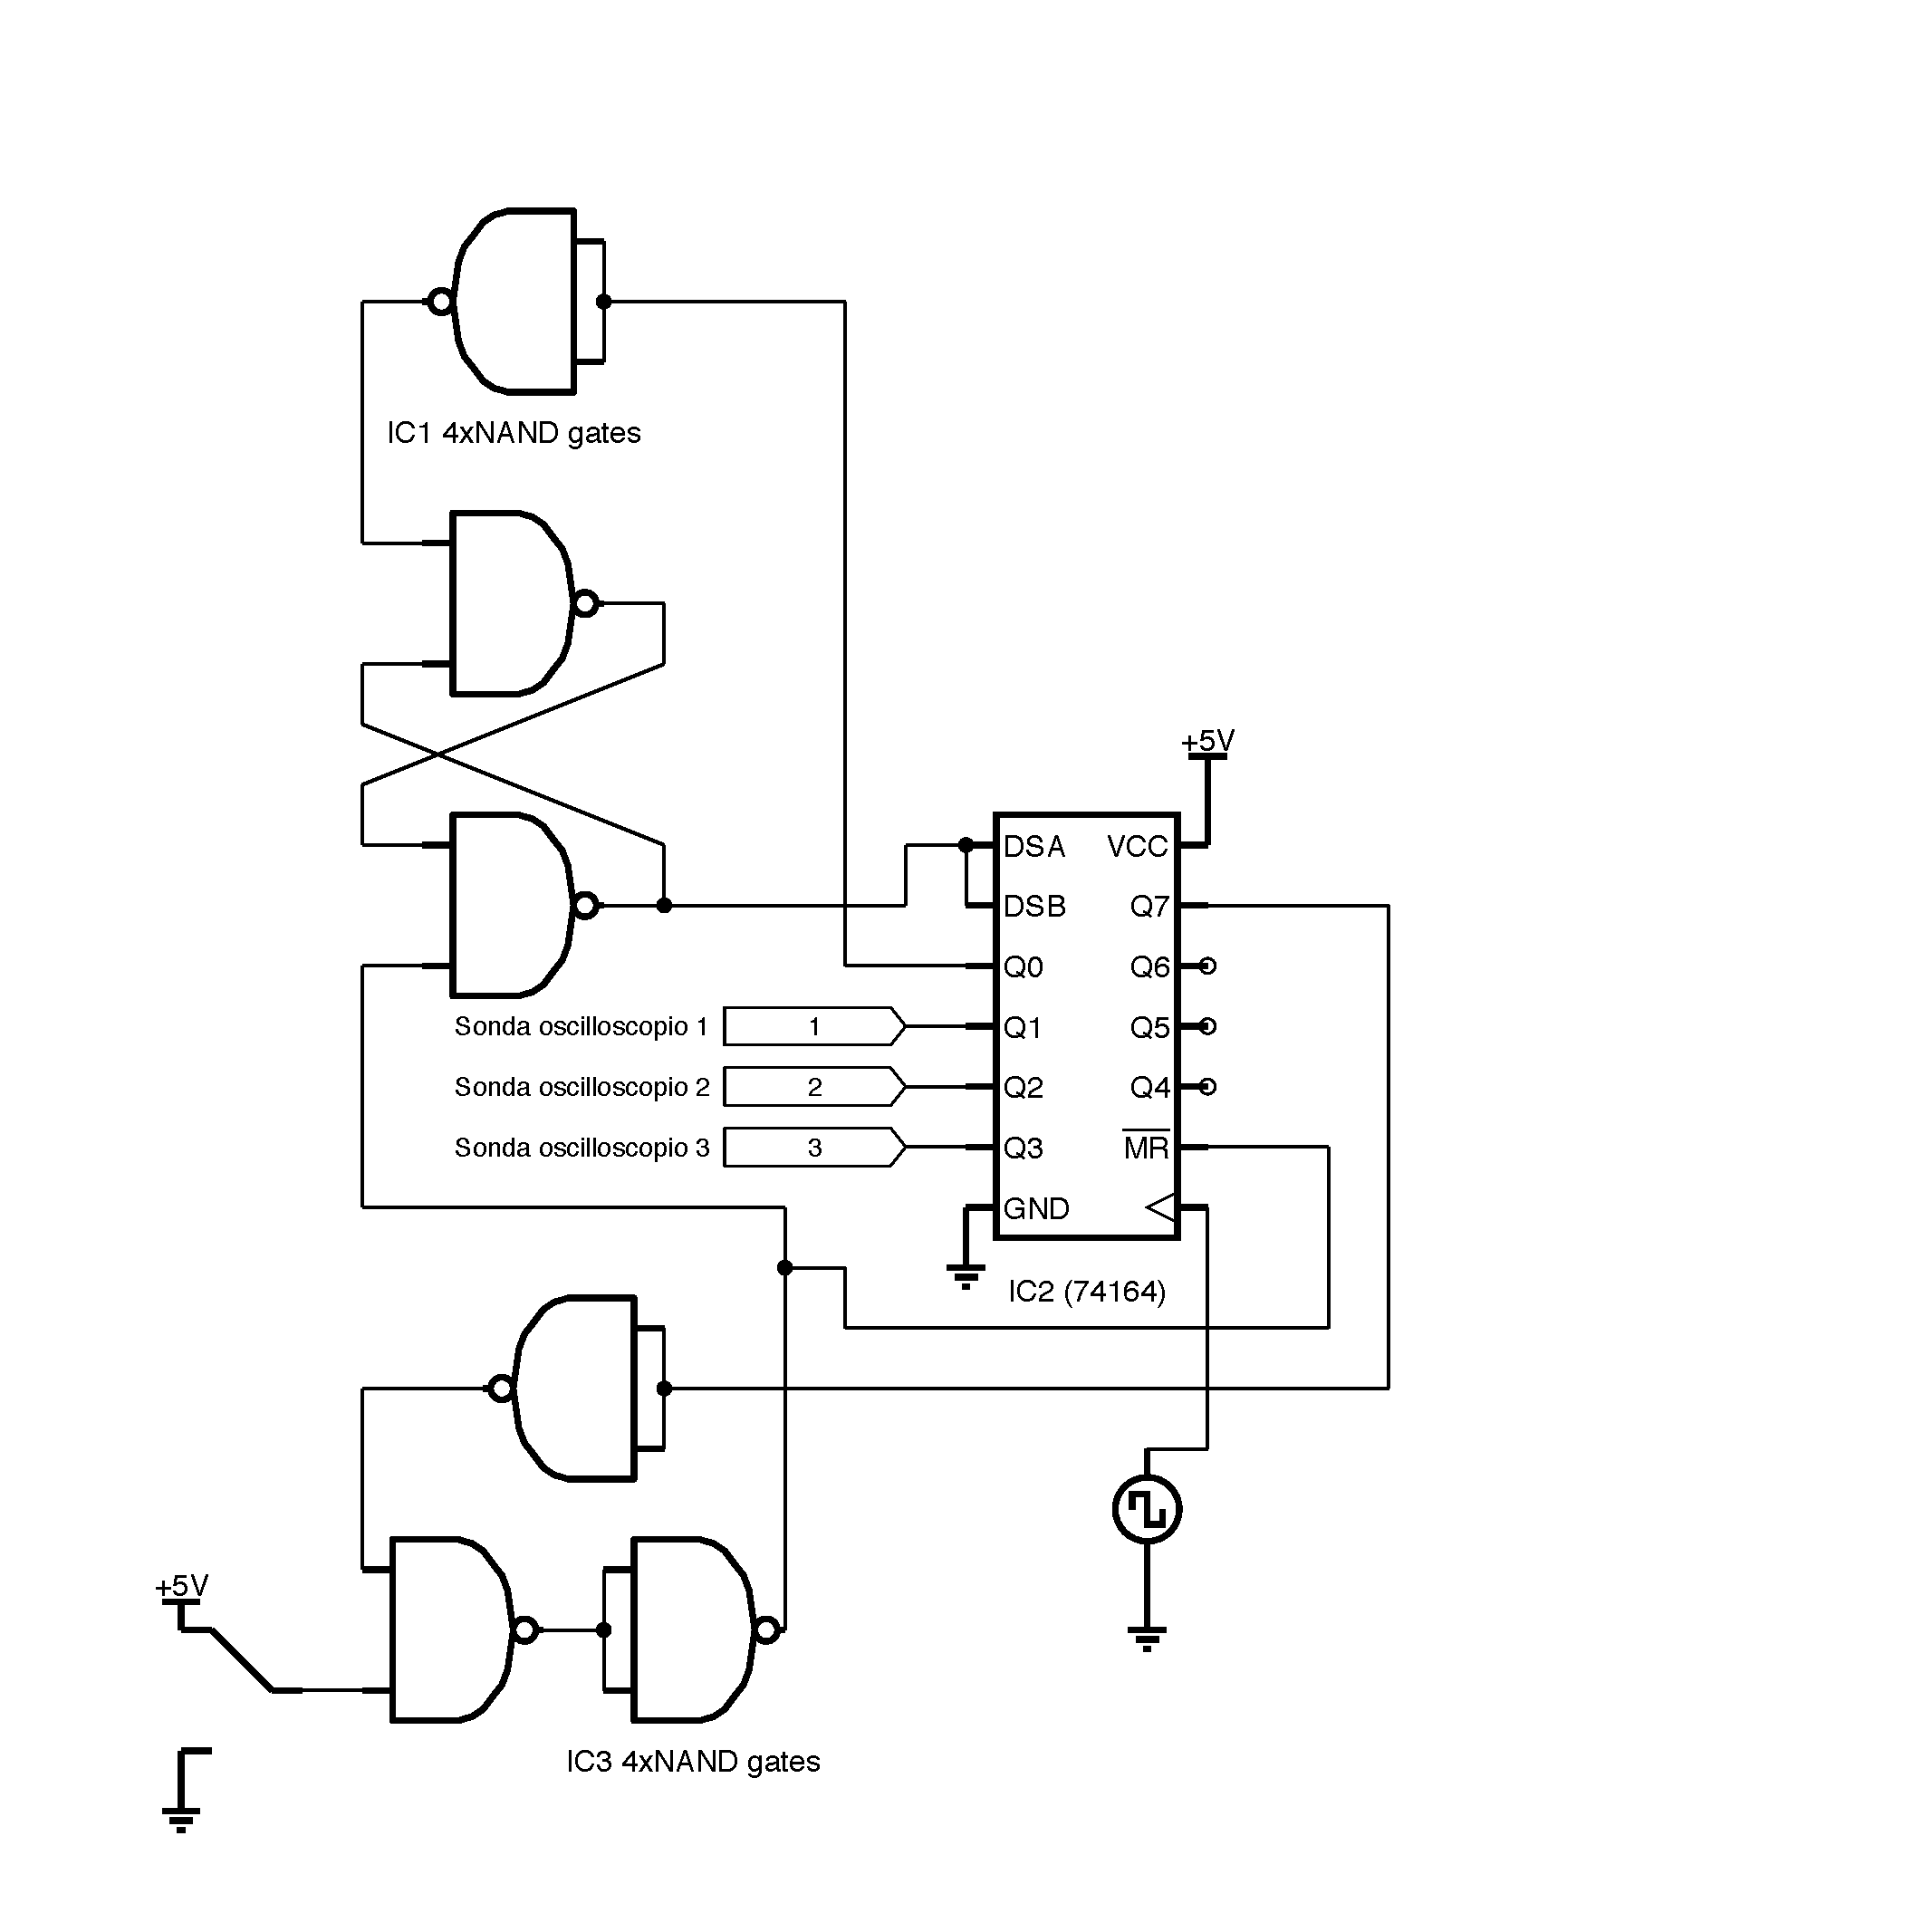
\includegraphics[width=0.50\textwidth]{sch-simulations/digital/output/shift-register.pdf}
\caption{Registro a scorrimento e circuito di controllo}
\label{fig:circuit_shift_register}
\end{center}
\end{figure}

Gli \textit{shift register} (registri a scorrimento) sono un tipo di circuito logico sequenziale sfruttato principalmente per l'archiviazione di dati digitali o per la lettura in parallelo di dati trasferiti in modalità seriale. Il registro utilizzato in laboratorio è realizzato mediante un gruppo di \textit{master-slave flip-flop} collegati in catena in modo che l'output di ogni blocco costituisca l'input del successivo. Tutti i flip-flop sono controllati da un segnale di clock e da un segnale di reset comune.
Ad ogni fronte di salita del clock (il registro utilizzato in laboratorio è del tipo \textit{positive-edge}) lo stato di ogni flip-flop viene trasferito al successivo, mentre il primo della catena viene inizializzato utilizzando i valori logici presenti agli ingressi A e B del registro. Lo stato di ciascun flip-flop può essere letto in modo asincrono in parallelo utilizzando le uscite {$Q_A$, ... , $Q_H$}. Il dispositivo utilizzato in laboratorio per la realizzazione dell'ADC è un registro ad 8 bit \textit{SN74LS164M} corredato da due circuiti logici ausiliari di controllo realizzati con porte NAND:
\begin{itemize}
    \item Il primo (quello che nello schema in figura \ref{fig:circuit_shift_register} è realizzato con l'integrato IC1) controlla l'inizializzazione del registro: quando il segnale di reset passa allo stato basso un flip-flop SR inizializza gli ingressi A e B del registro allo stato alto e attende il primo fronte di salita del clock che fa scorrere il registro di una posizione, a quel punto lo stato alto viene trasferito all'uscita $Q_0$ (o $Q_A$) il cui complemento logico esegue il reset del flip-flop riportando gli ingressi A e B al valore basso. 
    \item Il secondo (quello che nello schema in figura \ref{fig:circuit_shift_register} è realizzato con l'integrato IC3) è invece responsabile dell'operazione di RESET: quando il bit 1 con cui era stato inizializzato il registro raggiunge l'ultima uscita $Q_7$ (o $Q_H$) oppure quando il pulsante manuale di reset viene portato allo stato basso, il circuito porta il segnale di clear globale allo stato basso, effettuando così il reset di tutti i circuiti logici.
\end{itemize}

La figura seguente mostra la verifica effettuata in laboratorio sul corretto funzionamento di questo circuito: il canale 4 dell'oscilloscopio acquisisce il segnale di trigger (realizzato con il generatore di funzioni utilizzando un'onda quadra oscillante tra 0 V e 5 V con frequenza di 5 Hz) mentre i primi tre canali (come segnato nello schema in figura \ref{fig:circuit_shift_register}) sono collegati alle tre uscite del registro successive alla prima. Dopo aver effettuato il reset osserviamo che il registro viene inizializzato dal circuito di controllo con un solo bit allo stato alto e questo bit viene fatto scorrere fino alla fine, quando avverrà un nuovo reset. 


\begin{figure}[H]%[!ht]
\begin{center}
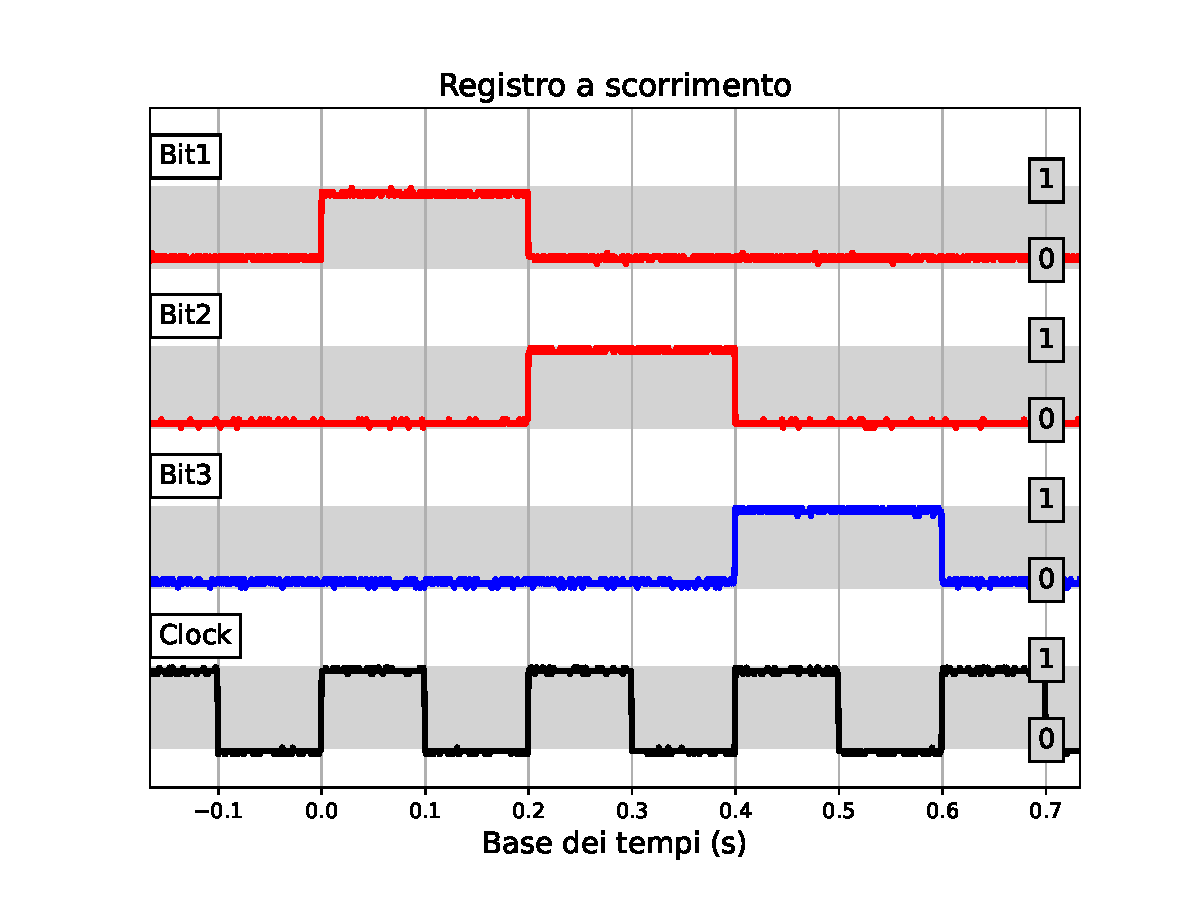
\includegraphics[trim = {0 0 0 0}, clip, width=0.50\textwidth]{analysis/output/reg_test.pdf}
\caption{BIT con transistor}
\label{fig:BIT_with_transistor}
\end{center}
\end{figure}

\subsection{Verifica del circuito di pilotaggio del DAC (J-K) e dello stadio analogico}
Descriviamo e verifichiamo ora il sottocircuito successivo che consente il funzionamento dell'ADC: il circuito di pilotaggio del DAC realizzato con flip-flop di tipo J-K. L'obiettivo di questo circuito è di effettuare il confronto del valore di ogni bit con la tensione da misurare mediante il pilotaggio del DAC, realizzando il processo di approssimazioni successive. 

\begin{figure}[H]%[!ht]
\begin{center}
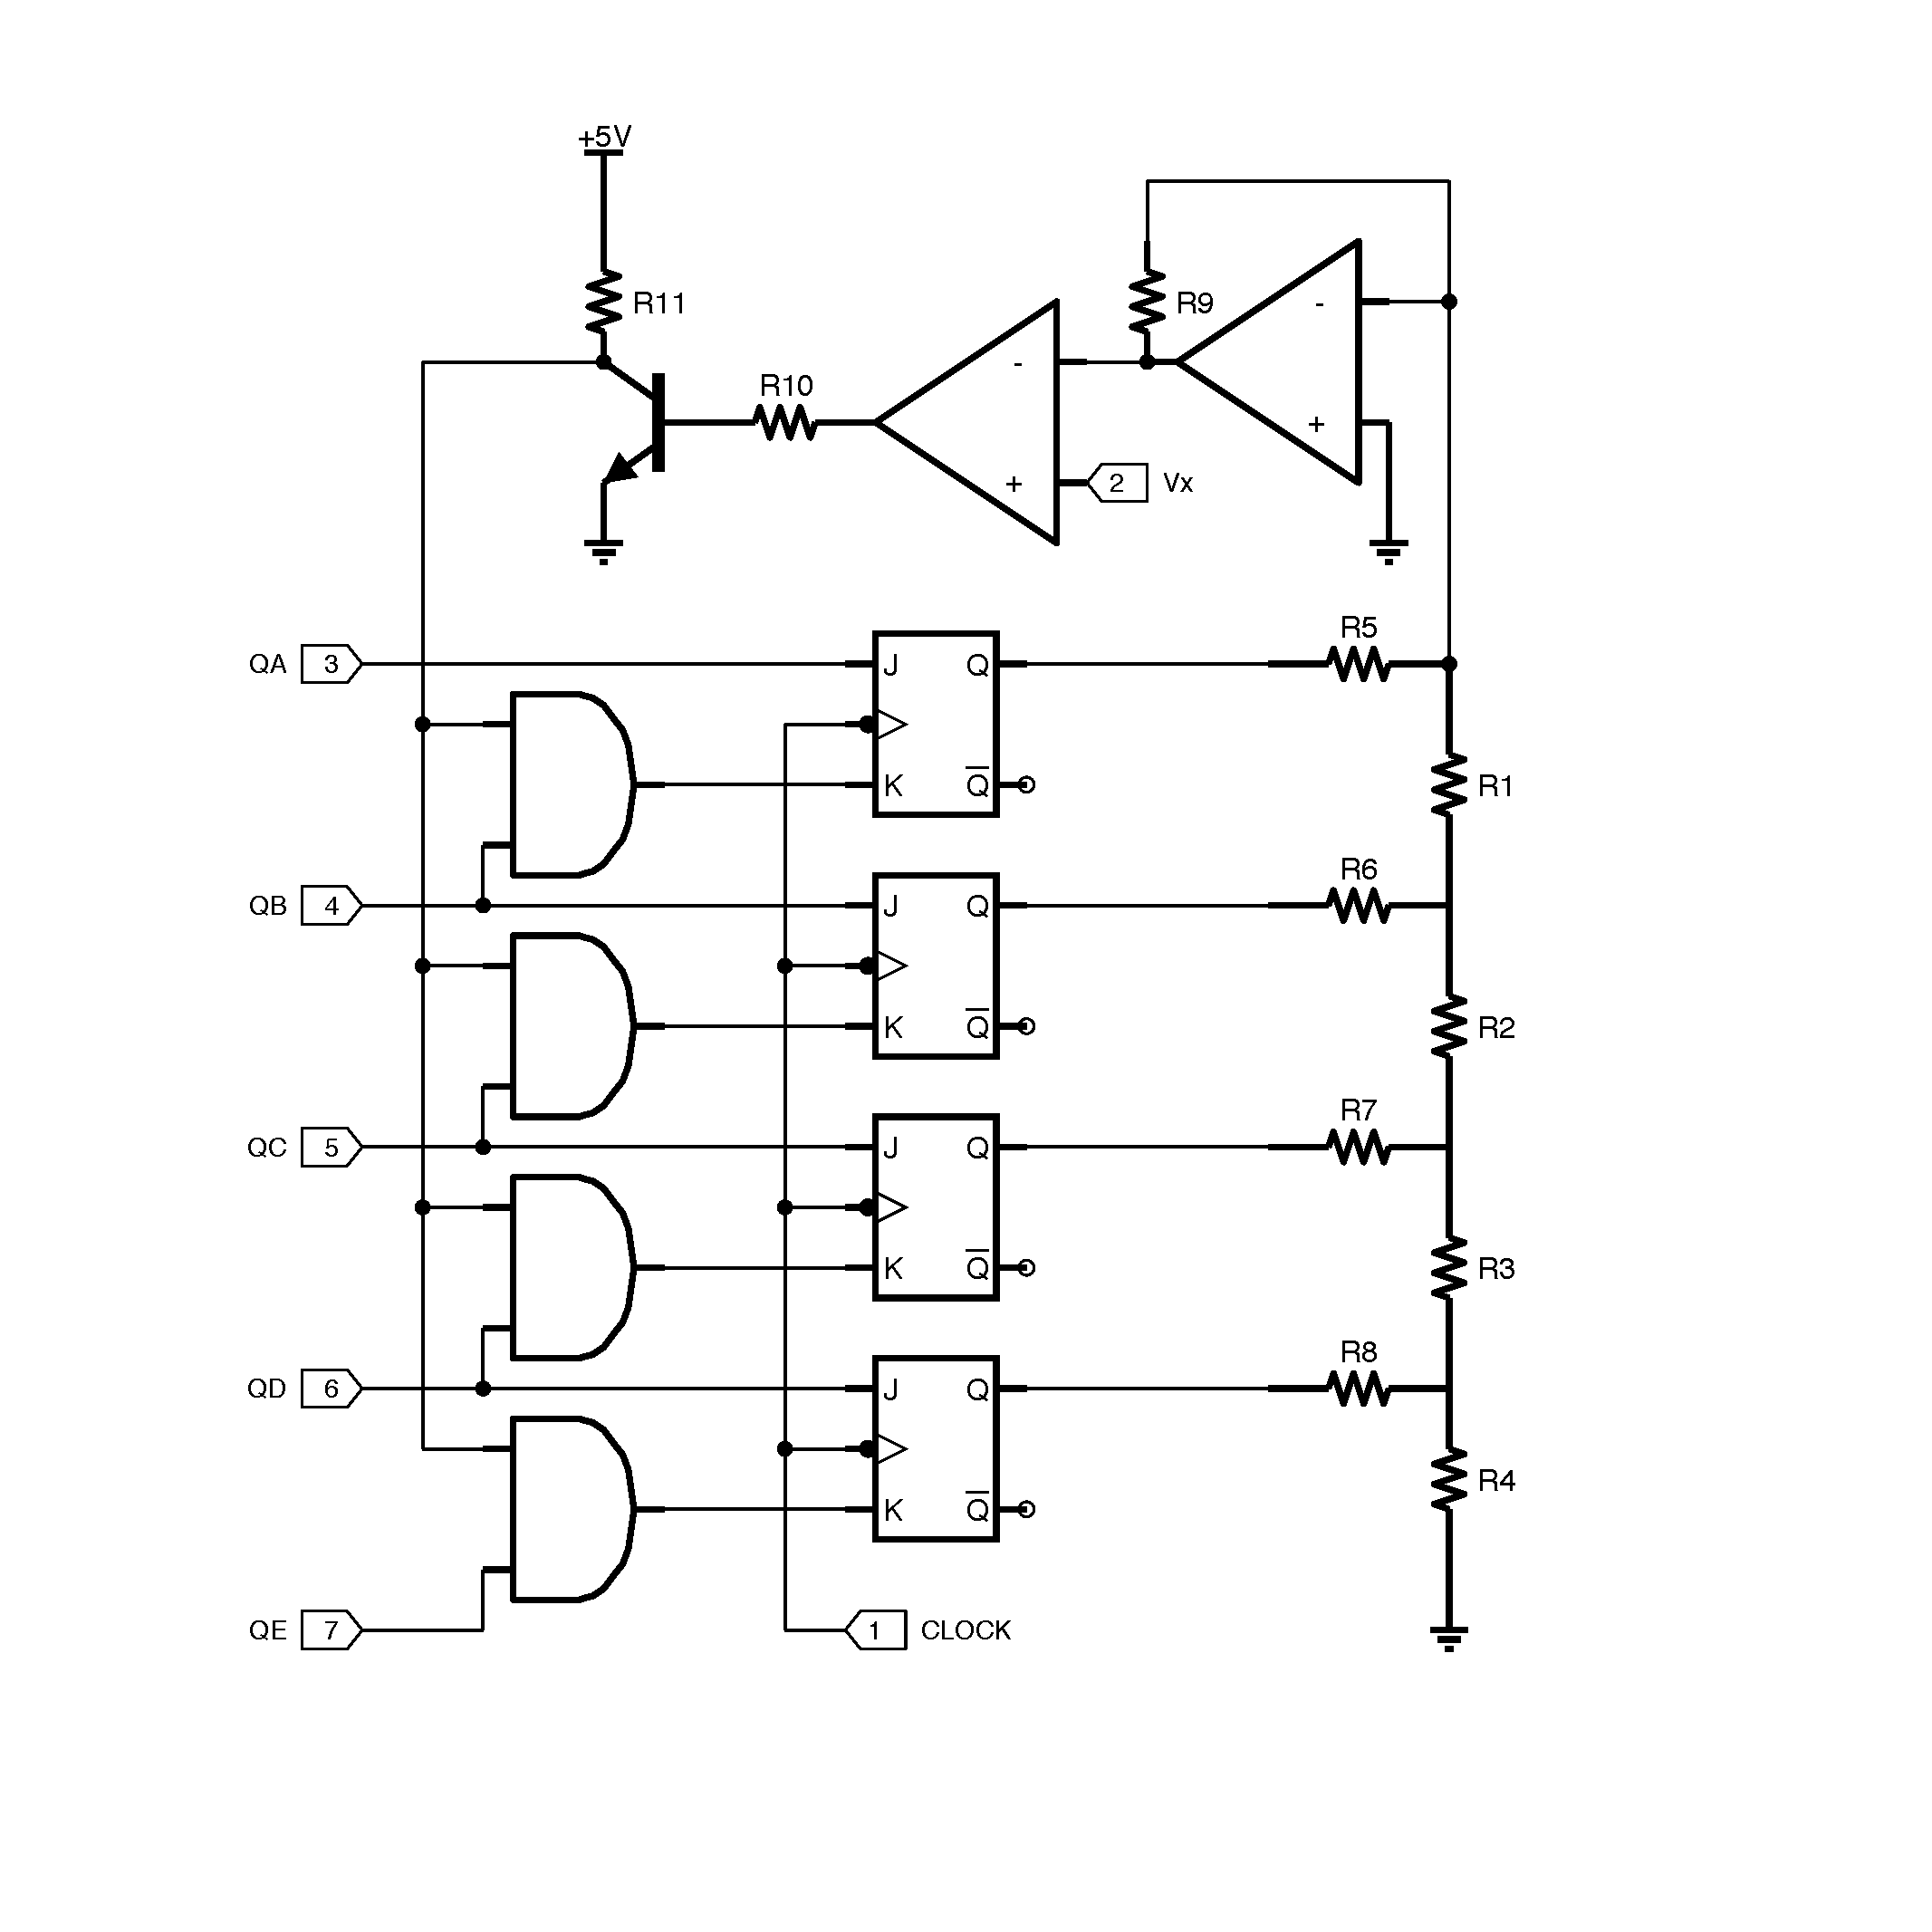
\includegraphics[width=0.48\textwidth]{sch-simulations/digital/output/DAC.pdf}
\caption{Circuito di controllo del DAC con flip-flop J-K e sezione analogica dell'ADC. $R_{base}$ = $R_{10}$ = (0.99 $\pm$ 0.01) $K\Omega$, $R_{collettore}$ = $R_{11}$ = (99 $\pm$ 1) $K\Omega$ }
\label{fig:circuit_DAC_JK_transistor}
\end{center}
\end{figure}

Il funzionamento è il seguente: ogni uscita del registro di scorrimento attiva il J di ciascun flip-flop e, con l'esclusione della prima, attiva il K del flip-flop precedente. Mentre l'operazione di set J è sempre effettuata, quella di reset K è eseguita solo se il complemento logico dell'uscita del comparatore è alto, perché ogni ingresso K non è direttamente collegato al registro, ma bensì attraverso una porta AND con il segnale logico proveniente dal comparatore. Il risultato è che ogni bit viene attivato, ma viene disattivato solo in base all'operazione di confronto, quindi al termine del ciclo di conversione lo stato delle uscite dei J-K costituirà la rappresentazione binaria del segnale quantizzato. 

La verifica in laboratorio si è svolta dapprima collegando le 4 uscite dei J-K ai 4 canali dell'oscilloscopio e forzando al livello basso il complemento logico dell'uscita del comparatore (si veda la figura \ref{fig:cumulative_BIT}), in questo caso, come atteso, osserviamo che in un ciclo di conversione tutti i bit vengono attivati e rimangono allo stato alto fino all'operazione di clear, che coinvolge anche i J-K.

Nella figura \ref{fig:cumulative_BIT_clk} osserviamo il medesimo scenario di funzionamento, ma questa volta la sonda collegata al canale 4 dell'oscilloscopio è stata collegata al clock e questo ci permette di osservare, per esempio, che la commutazione dei J-K avviene sul fronte di discesa. Per il corretto funzionamento dell'ADC è molto rilevante che le la commutazione del registro avvenga sul fronte di salita del clock, mentre quella dei J-K avvenga sul fronte di discesa, in questo modo quando i flip-flop leggono i loro ingressi J e K il registro li ha già sicuramente portati ad uno stato logico valido.

\begin{figure}[H]%[!ht]
\begin{center}
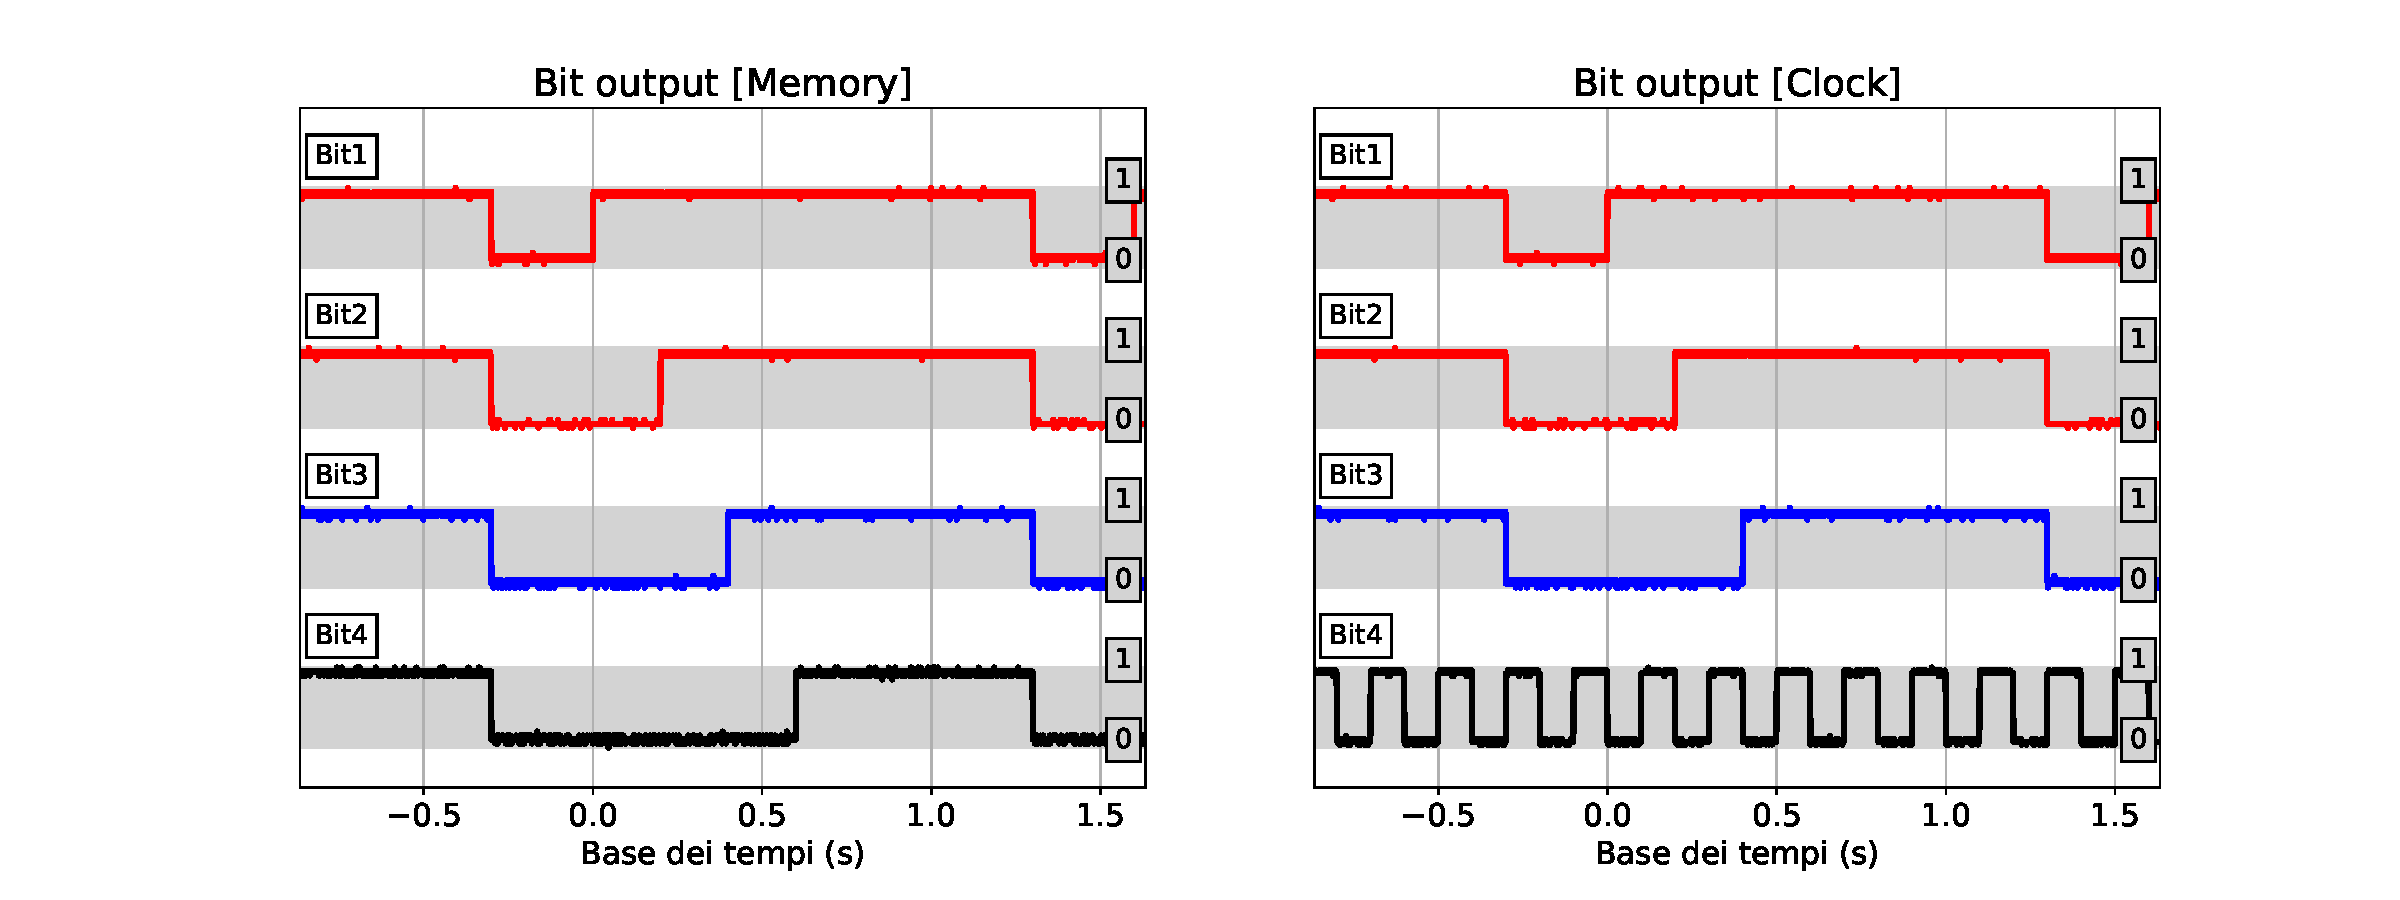
\includegraphics[trim = {100 0 550 0}, clip, width=0.43\textwidth]{analysis/output/cumulative_BIT.pdf}
\caption{Uscite dei flip-flop J-K quando il complemento logico del comparatore è allo stato basso}
\label{fig:cumulative_BIT}
\end{center}
\end{figure}

\vspace{-10mm}

\begin{figure}[H]%[!ht]
\begin{center}
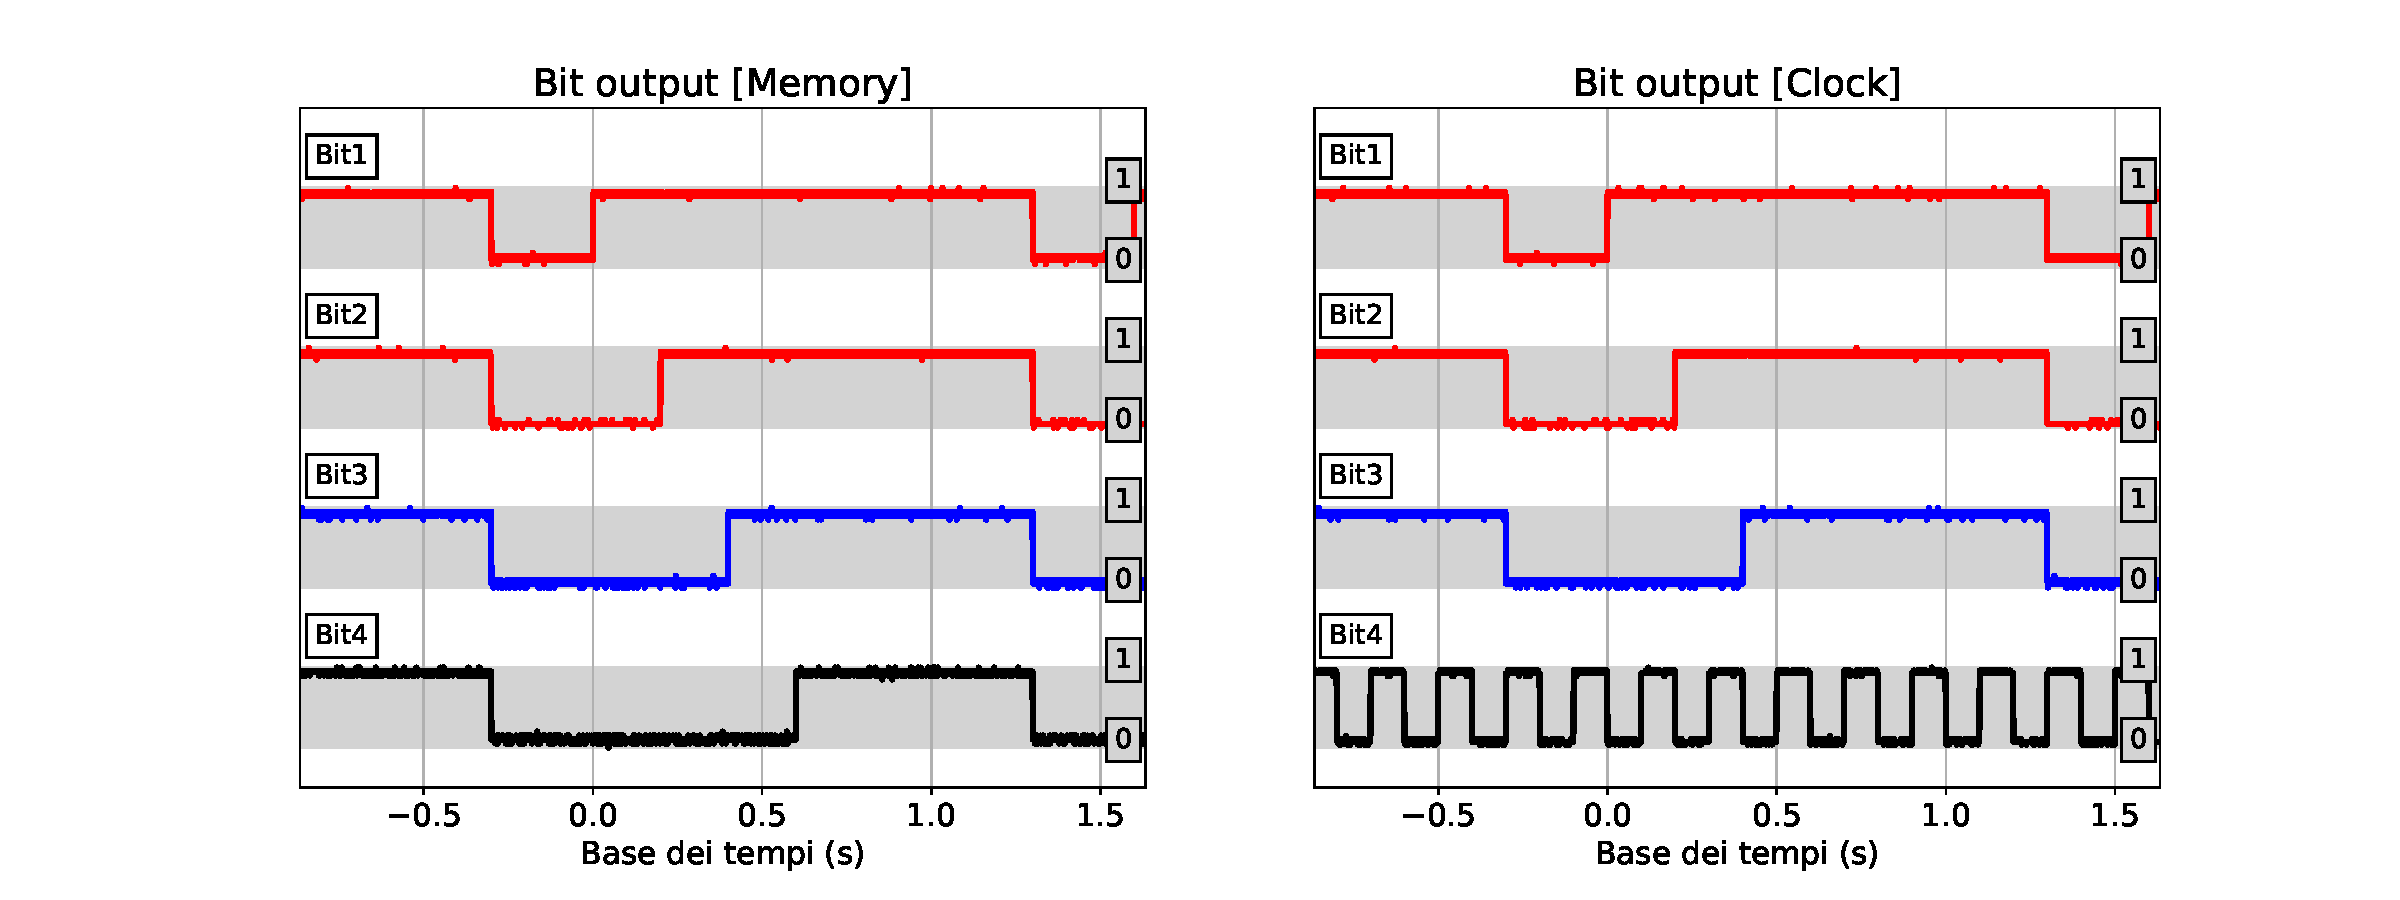
\includegraphics[trim = {600 0 100 0}, clip, width=0.39\textwidth]{analysis/output/cumulative_BIT.pdf}
\label{fig:cumulative_BIT_clk}
\end{center}
\end{figure}

\vspace{-7mm}

Nella figura seguente si osserva la medesima misura effettuata però forzando il complemento logico dell'uscita del comparatore allo stato alto. Le uscite delle porte AND che controllano gli ingressi K potranno quindi raggiungere lo stato alto e ogni bit verrà resettato sul fronte di discesa del \textit{clock} in cui viene settato il bit successivo.

\begin{figure}[H]%[!ht]
\begin{center}
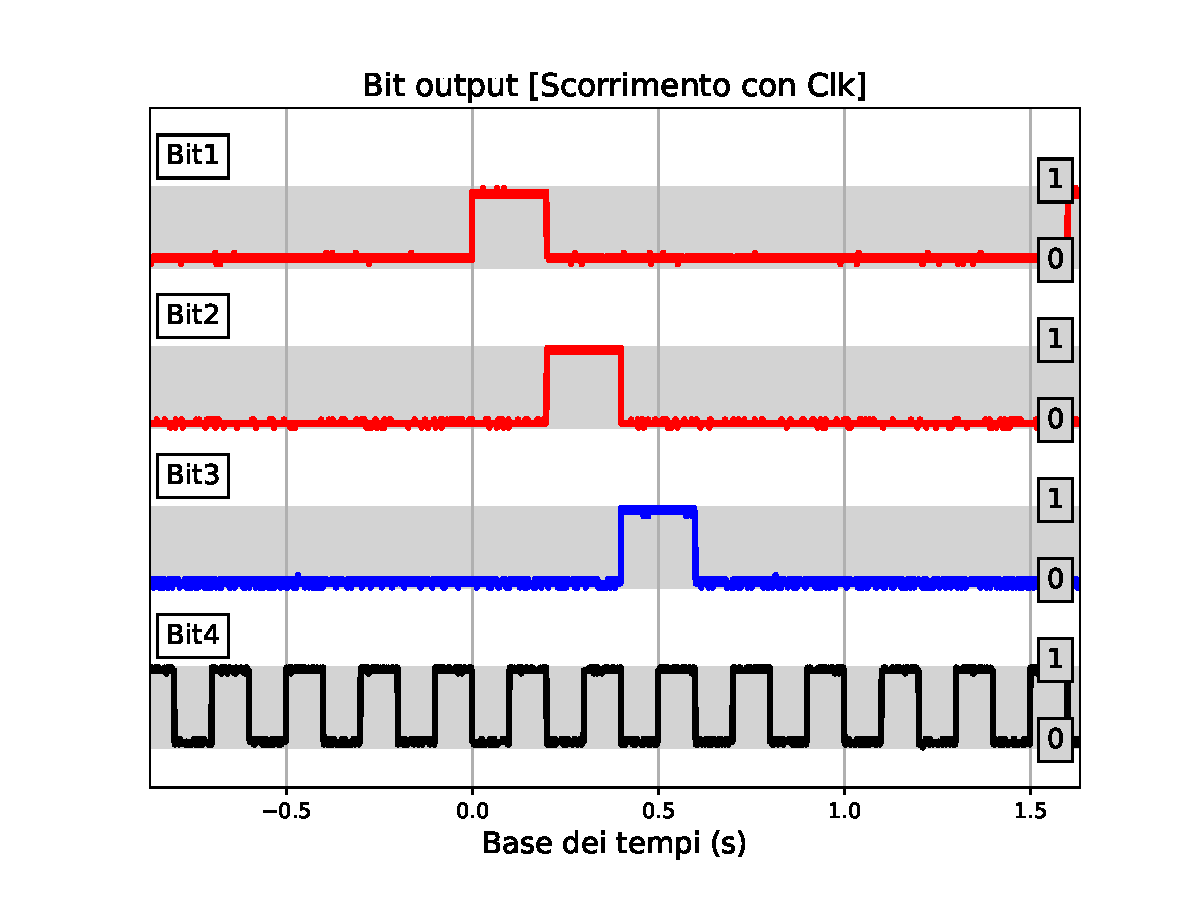
\includegraphics[width=0.48\textwidth]{analysis/output/BIT-shift-clk.pdf}
\label{fig:BIT_shift_clk}
\end{center}
\end{figure}

Per realizzare l'acquisizione seguente sono stati, invece, collegati i primi tre canali dell'oscilloscopio alle uscite dei J-K, ma l'ultimo canale è stato collegato alla base del transistor di interfaccia del comparatore, quindi mostra esattamente il risultato logico dell'operazione di confronto. Osserviamo che quando l'operazione di confronto restituisce 0 (uscita del DAC più alta del segnale in ingresso) le porte AND possono attivarsi e i bit vengono man mano resettati, mentre quando l'operazione di confronto restituisce 1 (uscita del DAC più bassa del segnale in ingresso) i bit rimangono attivi quando la conversione giunge al termine.

\begin{figure}[H]%[!ht]
\begin{center}
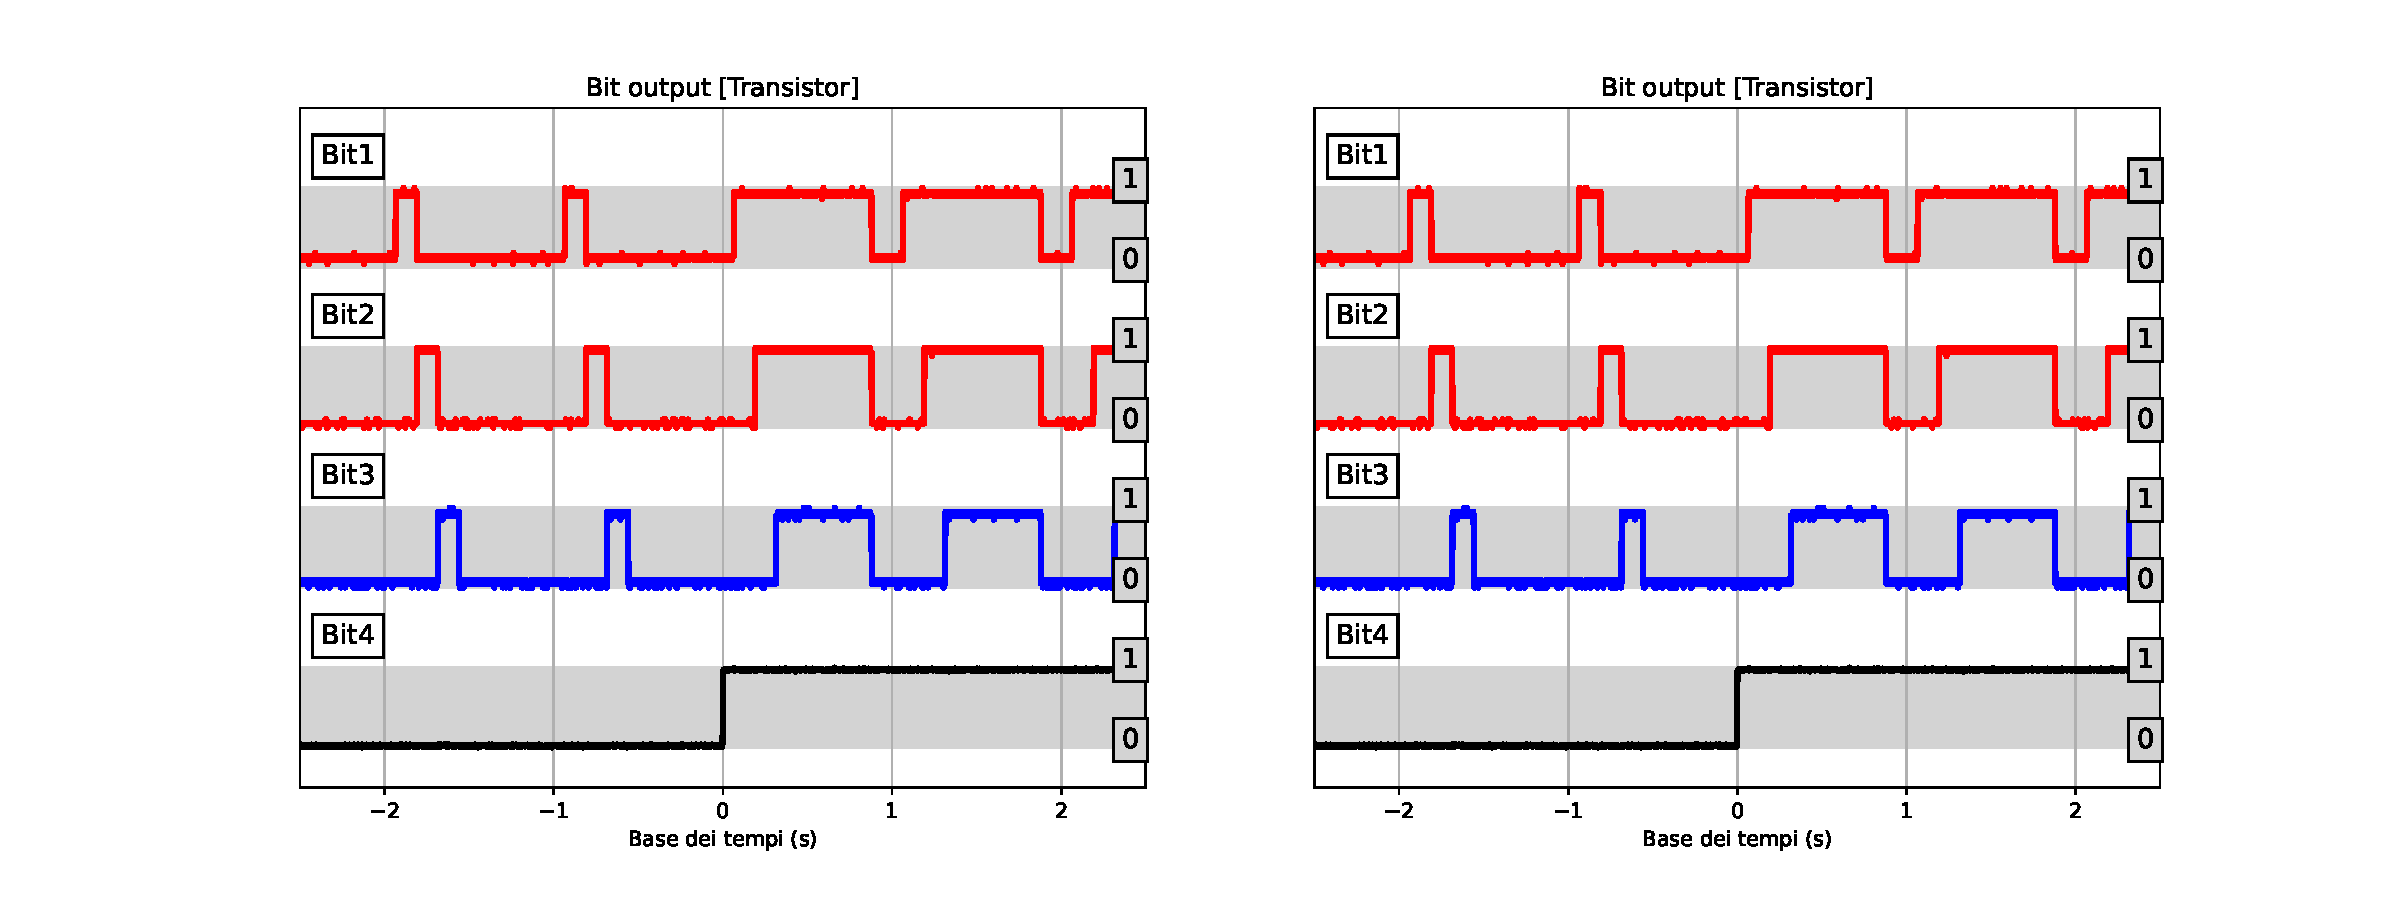
\includegraphics[trim = {570 0 0 0}, clip, width=0.50\textwidth]{analysis/output/cumulative_BIT_with_transistor.pdf}
\caption{Uscite dei J-K sui primi tre ingressi dell'oscilloscopio, sul 4 il livello logico dell'uscita del comparatore, cioè l'alimentazione della base del transistor.}
\label{fig:Comparator-output}
\end{center}
\end{figure}

\subsection{Convertitore digitale-analogico}
Il confronto tra il valore logico rappresentato dalle uscite dei flip-flop J-K e il segnale analogico in ingresso è possibile solo grazie ad un DAC di tipo R-2R pilotato da tali uscite. Il DAC è realizzato mediante resistori discreti dei valori riportati a seguire che realizzano una rete che alimenta l'ingresso invertente di un amplificatore operazionale retroazionato a guadagno unitario (LM741). L'uscita di tale amplificatore operazionale controlla l'ingresso invertente di un secondo componente identico che lavora però in configurazione ad anello aperto, realizzando così il comparatore vero e proprio, dal momento che il suo ingresso non invertente costituisce l'ingresso analogico dell'ADC. Come anticipato, si rende necessaria l'introduzione di un transistor di interfaccia con tre funzioni:
\begin{itemize}
    \item Adattare i livelli di tensione $\pm$ 15 V ai livelli logici TTL 0V - 5V
    \item Effettuare un'operazione di "NOT" logico
    \item Grazie all'amplificazione dovuta alla configurazione ad emettitore comune rendere più ripido il fronte di commutazione dell'uscita del comparatore, consentendo all'ADC di lavorare a frequenze più elevate.
\end{itemize}


\begin{table}[H]
\begin{center}
\caption{Resistori utilizzati per il DAC}
\begin{tabular}{c|c}
\hline
Nome in fig.\ref{fig:nyquist_mcu_cumulative} & R (k$\Omega $) \\ \hline
R1  & $1.00 \pm 0.01$ \\
R2  & $1.00 \pm 0.01$ \\
R3  & $1.00 \pm 0.01$ \\
R4  & $2.01 \pm 0.02$ \\
R5  & $1.94 \pm 0.02$ \\
R6  & $1.94 \pm 0.02$ \\
R7  & $2.01 \pm 0.02$ \\
R8  & $1.99 \pm 0.02$ \\

\label{tab:resistori_dac}
\end{tabular}
\end{center}
\end{table}


\subsection{Caratteristica di trasferimento del transistor di interfaccia}
Nella \textit{figura \ref{fig:VTC-bjt}} è riportata la \textit{VTC} del transistor NPN PN2222A appena descritto nel paragrafo precedente. La misurazione della caratteristica di trasferimento in tensione ha permesso di confermare che effettivamente il componente agisce da inverter logico. In laboratorio si è potuto osservare, inoltre, che il fronte di discesa della tensione di collettore quando il transistor passa dalla regione di interdizione a quella di saturazione risulta essere nettamente più ripido rispetto al fronte di salita della tensione di base (proveniente dall'uscita dall'OPA del comparatore) e questo permette di far lavorare l'ADC a frequenze di \textit{clock} più elevate. Infine, come desiderato, si è ottenuta la compatibilità con lo standard TTL, dato che la $V_{out}$ (tensione di collettore) si trova sempre compresa tra 0 V e 5 V. Per misurare la caratteristica, la base del transistor è stata alimentata con una rampa positiva tra -15 V e +15 V attraverso la resistenza $R_{10}$ dal generatore di funzioni e su questo segnale è stata collegata la prima sonda dell'oscilloscopio (asse orizzontale), la seconda sonda (asse verticale) è stata invece collegata al collettore del transistor.

\begin{figure}[H]%[!ht]
\begin{center}
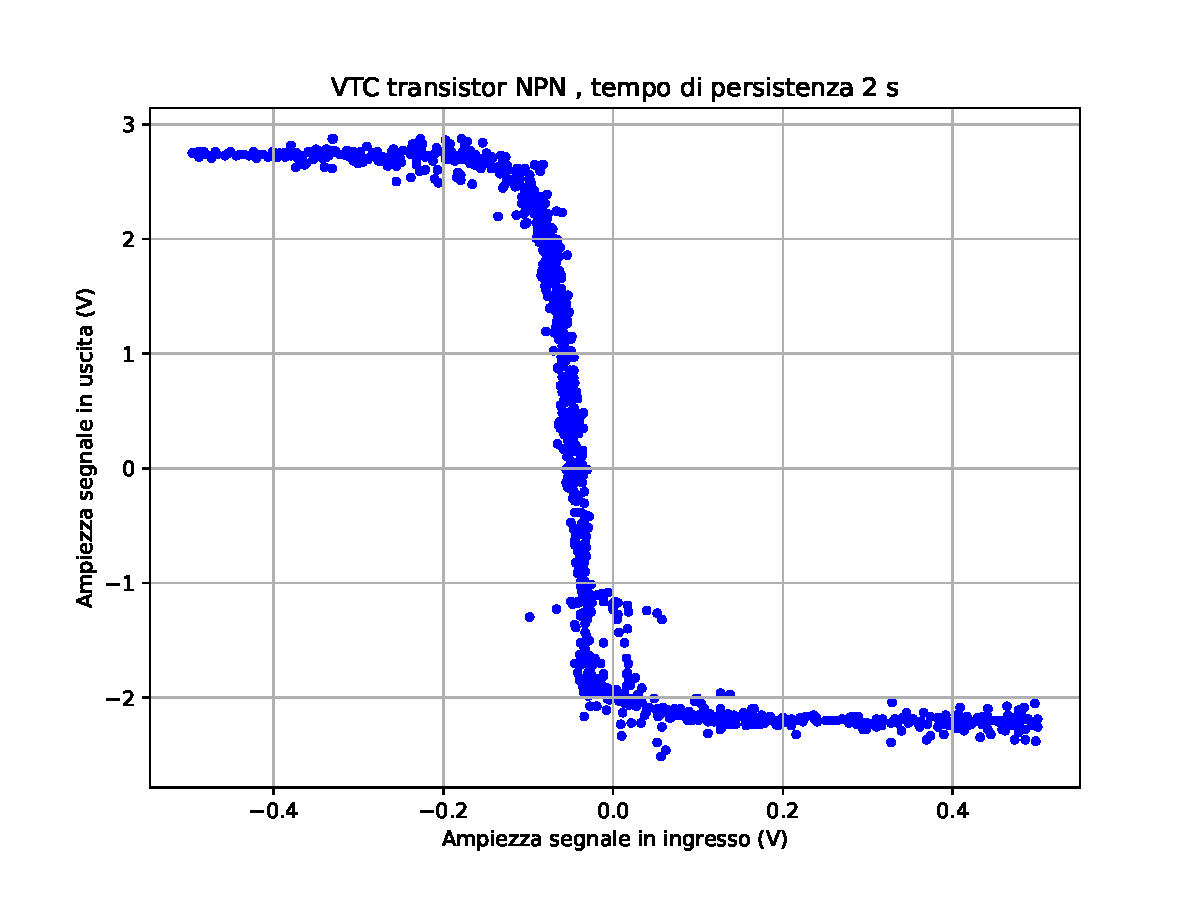
\includegraphics[width=0.45\textwidth]{analysis/output/NPN-XY.pdf}
\caption{Caratteristica di trasferimento in tensione base-collettore del transistor di interfaccia.}
\label{fig:VTC-bjt}
\end{center}
\end{figure}


\subsection{Caratteristiche del segnale di \textit{clear}}
Tutti i componenti digitali sincroni utilizzati dispongono di un ingresso a cui è possibile fornire un segnale di \textit{clear} che quando è portato al livello basso effettua il reset del dispositivo. Nei circuiti logici dell'ADC che stiamo esaminando i pin di clear sono collegati tutti in parallelo e tale segnale è prodotto dal circuito di controllo del registro che utilizza l'integrato (che nello schema generale è denominato U8). Come già discusso in precedenza, tale circuito di controllo mantiene basso il livello del clear quando l'interruttore di reset è portato a massa oppure quando il registro porta al livello alto l'uscita $Q_H$ o $Q_7$. Si nota immediatamente quindi che il segnale di clear è destinato a rimanere al livello basso per un tempo estremamente breve, poiché non appena il registro effettua il reset l'uscita suddetta passerà immediatamente al livello basso. Risulta quindi interessante esaminare la durata del segnale, che da risulta essere $\Delta \tau$ = (46 $\pm$ 5) ns ed è rappresentata nella terza traccia a partire dall'alto nella figura seguente.

\begin{figure}[H]%[!ht]
\begin{center}
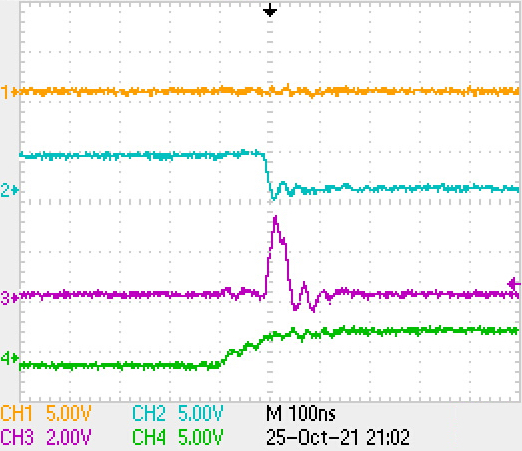
\includegraphics[width=0.40\textwidth]{data-source/25-10-21/clear.jpg}
\caption{Ritardo di propagazione attraverso i circuiti logici di U8 del segnale di clear}
\label{fig:clear-delay}
\end{center}
\end{figure}

%%%%%%%%%%%%%%%%%%%%%%%%%%%%%%%%%%%%%%%%%%%%%%%%%%%%%%%%%%%%%

\section{Calibrazione del DAC}

Un DAC ideale converte il codice digitale in ingresso in un segnale analogico ad esso proporzionale in uscita. Nei dispositivi reali, tuttavia, il segnale in uscita è soggetto sia a distorsioni sul guadagno che a offset non previsti che possono provenire da varie fonti, quali la tolleranza dei resistori della rete R-2R, non linearità degli amplificatori operazionali, non uniformità delle caratteristiche dei J-K.
È pertanto necessario calibrare il DAC per verificare che, entro un certo limite di significatività, esso rispecchi il comportamento atteso.
Alimentando con la tensione +5 V proveniente dall'alimentatore i singoli bit, si sono misurati i valori dei segnali in uscita per ciascuno dei 16 codici binari supportati. I valori di tensione misurati sono mostrati in tabella \ref{tab:calibrazione_dac}), mentre in figura \ref{fig:graph_calibrazione_dac} è visibile il grafico con la relativa retta di calibrazione interpolante.


Eseguendo un fit lineare ($y = mx + q$) si sono ottenuti i seguenti parametri: 
\[ m = (-0.211 \pm 0.001) V \] 
\[ q = (-0.01 \pm 0.01) \ V \] 
$ \chi^{2} = 0.006 $ con p-value pari a $0.99$ con 14 gradi di libertà.

\begin{figure}[H]%[t]
\centering
\begin{center}
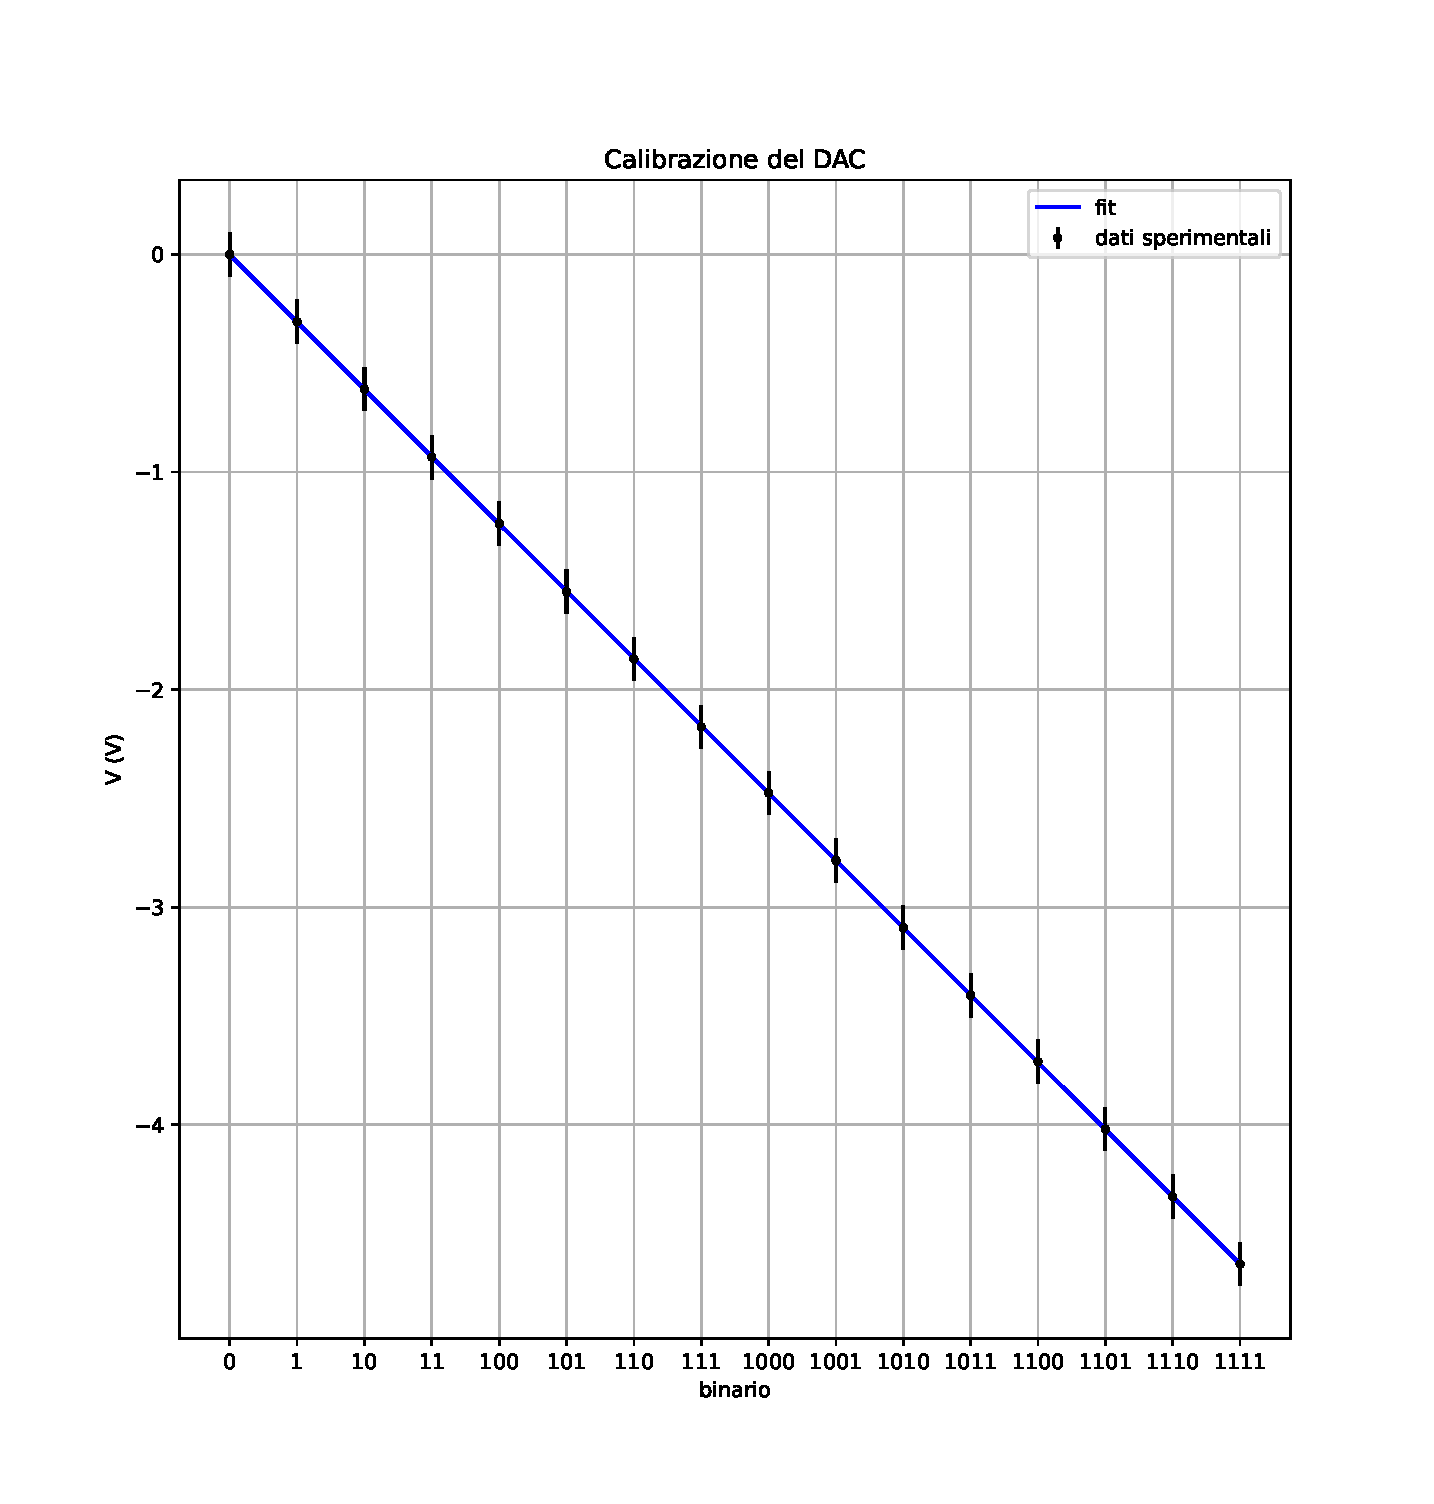
\includegraphics[width=0.51\textwidth]{analysis/output/calibrazione_dac.pdf}
\end{center}
\caption{Retta di calibrazione del DAC, i punti corrispondono alle tensioni misurate all'uscita quando i bit di ingresso vengono portati ai livelli logici rappresentati sull'asse orizzontale.}
\label{fig:graph_calibrazione_dac}
\end{figure}

Il test del chi quadro conferma che i dati sperimentali sono ben descritti da una relazione lineare, e dunque comportamento del circuito DAC risulta conforme alle aspettative. Per un valore in ingresso nullo ci si attende un valore in uscita nullo, cioè una retta passante nell'origine degli assi. Il valore di $q$ è risultato compatibile con lo 0, come confermato dal test Z che ha riportato il seguente valore della variabile statistica $Z = 1 $ con $ Z_c = 1.96$.

Avendo verificato che il DAC realizzato ha un comportamento sufficientemente lineare entro le incertezze sperimentali, procediamo a collegarlo ai restanti circuiti digitali completando l'assemblaggio.


%%%%%%%%%%%%%%%%%%%%%%%%%%%%%%%%%%%%%%%%%%%%%%%%%%%%%%%%%%%%%

%Un minimo di introduzione in cui si dice che ora abbiamo finito di montare tutti i sottocircuiti, l'ADC è completo e passiamo ora alla sua calibrazione. -- Questo infatti è il punto della relazione in cui termina la discussione dei sottocircuiti e comincia la caratterizzazione vera e propria del DAC %%
\section{Campionamento di tensioni continue e calibrazione dell'ADC}
Dopo aver analizzato singolarmente i circuiti costitutivi dell'ADC, si procede ora alla caratterizzazione dell'apparato nel suo complesso.
In primo luogo si desidera verificare che esso rispetti la caratteristica di linearità. L'ADC deve infatti convertire i segnali in ingresso in segnali direttamente proporzionali in uscita. Si intende ottenere la curva di calibrazione dell'ADC determinando con quale precisione si possa considerare lineare.

Si effettua una presa dati dei valori di tensione che corrispondono alle soglie di transizione tra due codici adiacenti. Per misurare tali tensioni si visualizzano sull'oscilloscopio il segnale in uscita dal comparatore e il segnale in uscita dal DAC e si fa variare utilizzando un potenziometro multigiro lineare (vedi \cite{K}) da R = (10.3 $\pm$ 0.1) $K\Omega$ la tensione in ingresso fino ad attraversare la soglia che determina il passaggio al codice successivo. La tensione di soglia è misurata con il multimetro, collegato in parallelo all'ingresso dell'ADC e la soglie sono sempre attraversate riducendo la tensione verso lo zero, poiché dispongono di una piccola isteresi indesiderata.
Nella tabella in appendice \ref{tab:calibrazione_adc} sono riportati i valori di tensioni sopracitati.

Ci si attende che tali valori siano distribuiti lungo una retta. In figura \ref{fig:graph_calibrazione_adc} è riportato il grafico interpolato.

\vspace{-5mm}

\begin{figure}[H]%[t]
\centering
\begin{center}
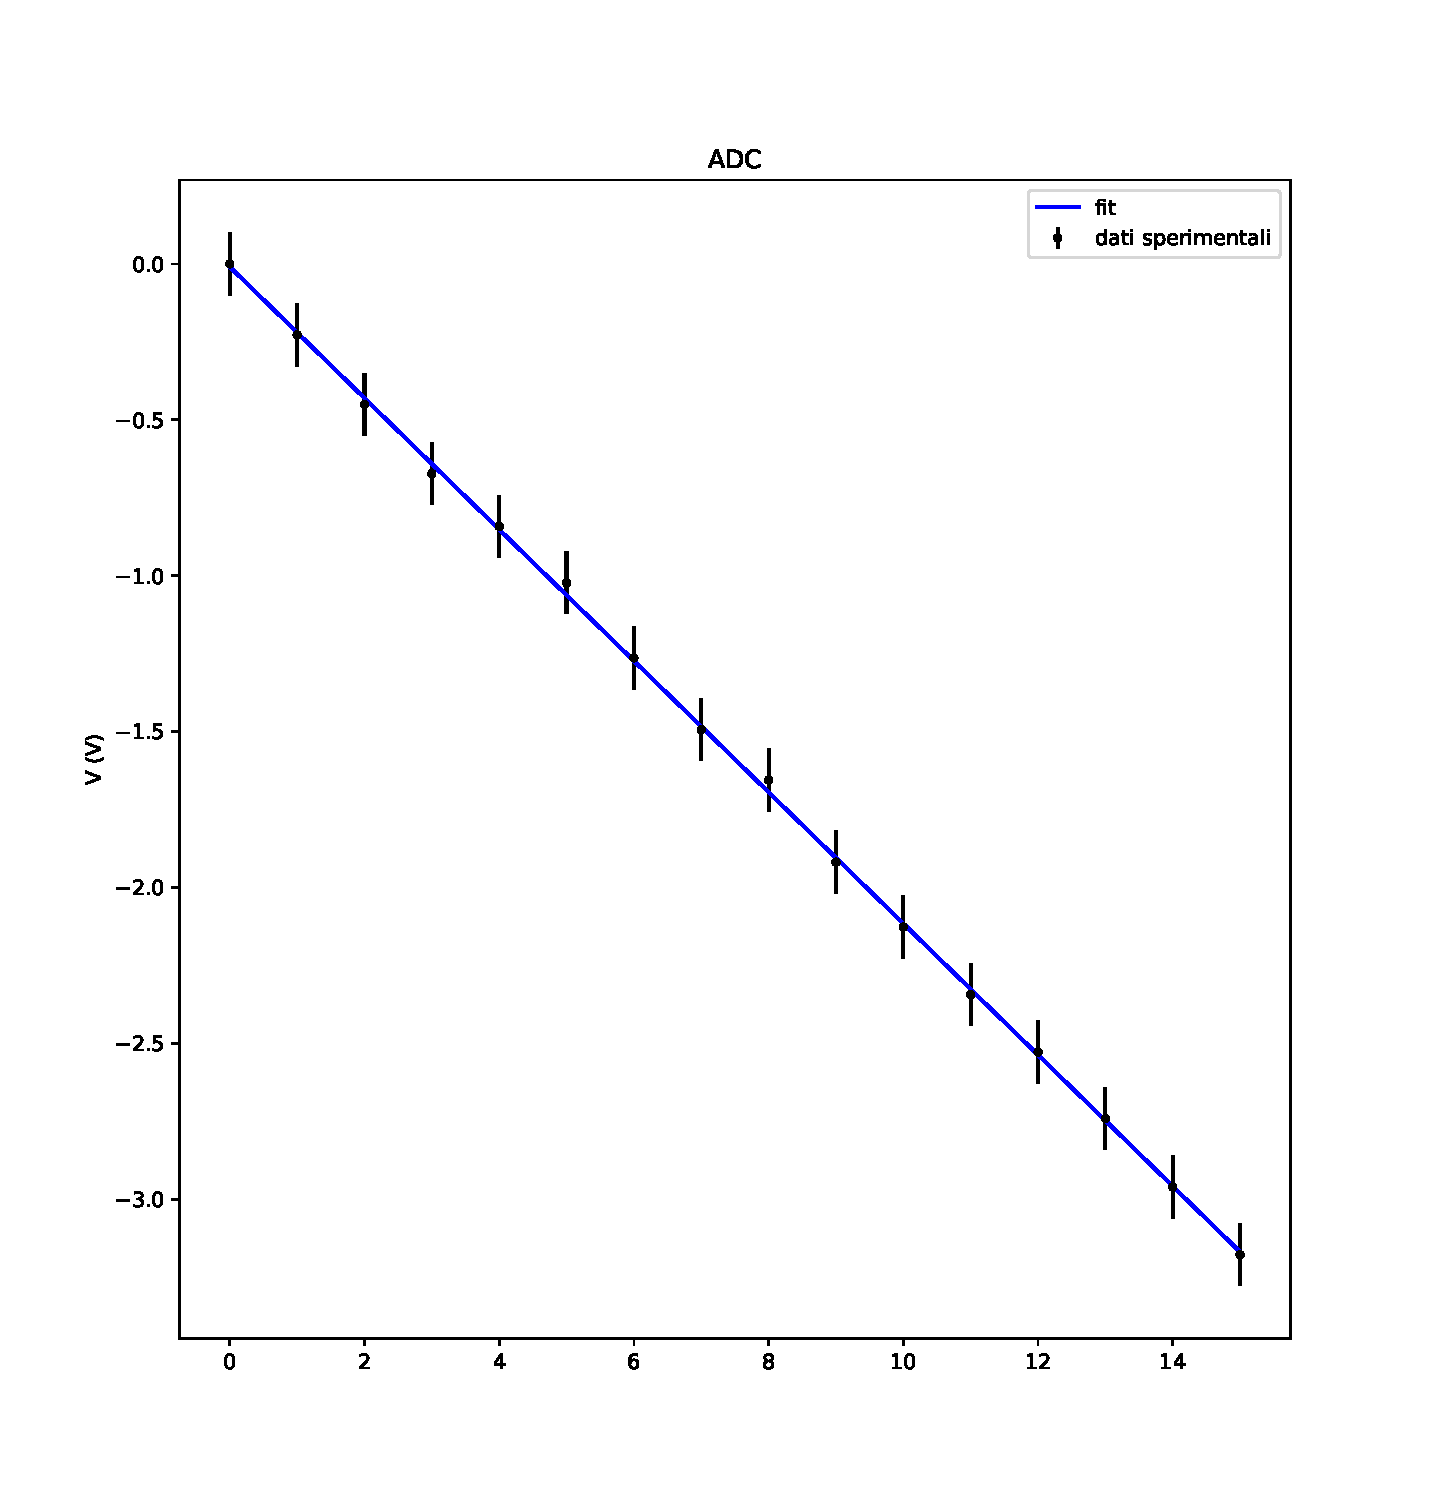
\includegraphics[width=0.51\textwidth]{analysis/output/calibrazione_adc.pdf}
\end{center}
\caption{Retta di calibrazione dell'ADC, i punti corrispondono alle soglie in cui cambia il codice binario restituito facendo variare la tensione in ingresso dal valore più negativo fino a 0 V.}
\label{fig:graph_calibrazione_adc}
\end{figure}

Eseguendo un fit lineare il minimizzatore restituisce i seguenti parametri:
\[ m = (-0.3092 \pm 0.0001) V \] 
\[ q = (-0.02 \pm 0.01) \ V \] 
$ \chi^{2} = 0.57 $ con p-value pari a $0.99$ con 14 gradi di libertà.
\newline
Il test del chi quadro conferma anche in questo caso la linearità dei dati. La variabile statistica $\chi^2$ è tuttavia di modulo molto basso ($0.57 << 14$), indicando una possibile sovrastima degli errori sulle tensioni misurate. Si segnala dunque che sarebbe opportuno ripetere l'analisi cambiando il metodo impiegato per individuare la soglia di transizione tra codici. Qui come errore è stato utilizzato quello relativo all'oscilloscopio, poiché è questo strumento che segnalando l'attraversamento delle soglie, decide quando effettuare la lettura della tensione. Entro i limiti dell'analisi effettuata si può affermare che l'ADC ha un comportamento lineare.
L'intercetta invece ha un valore incompatibile con lo 0 ($Z = 2 > Z_c = 1.96$). Ci si attende che la retta passi nell'origine perché a segnale nullo in ingresso corrisponda un segnale nullo in uscita. Si può dunque affermare che vi sia un errore di offset sui dati misurati, pari al valore di $q$, che non rientra nelle incertezze sperimentali.

\clearpage


\begin{figure*}[t]%[t]
\centering
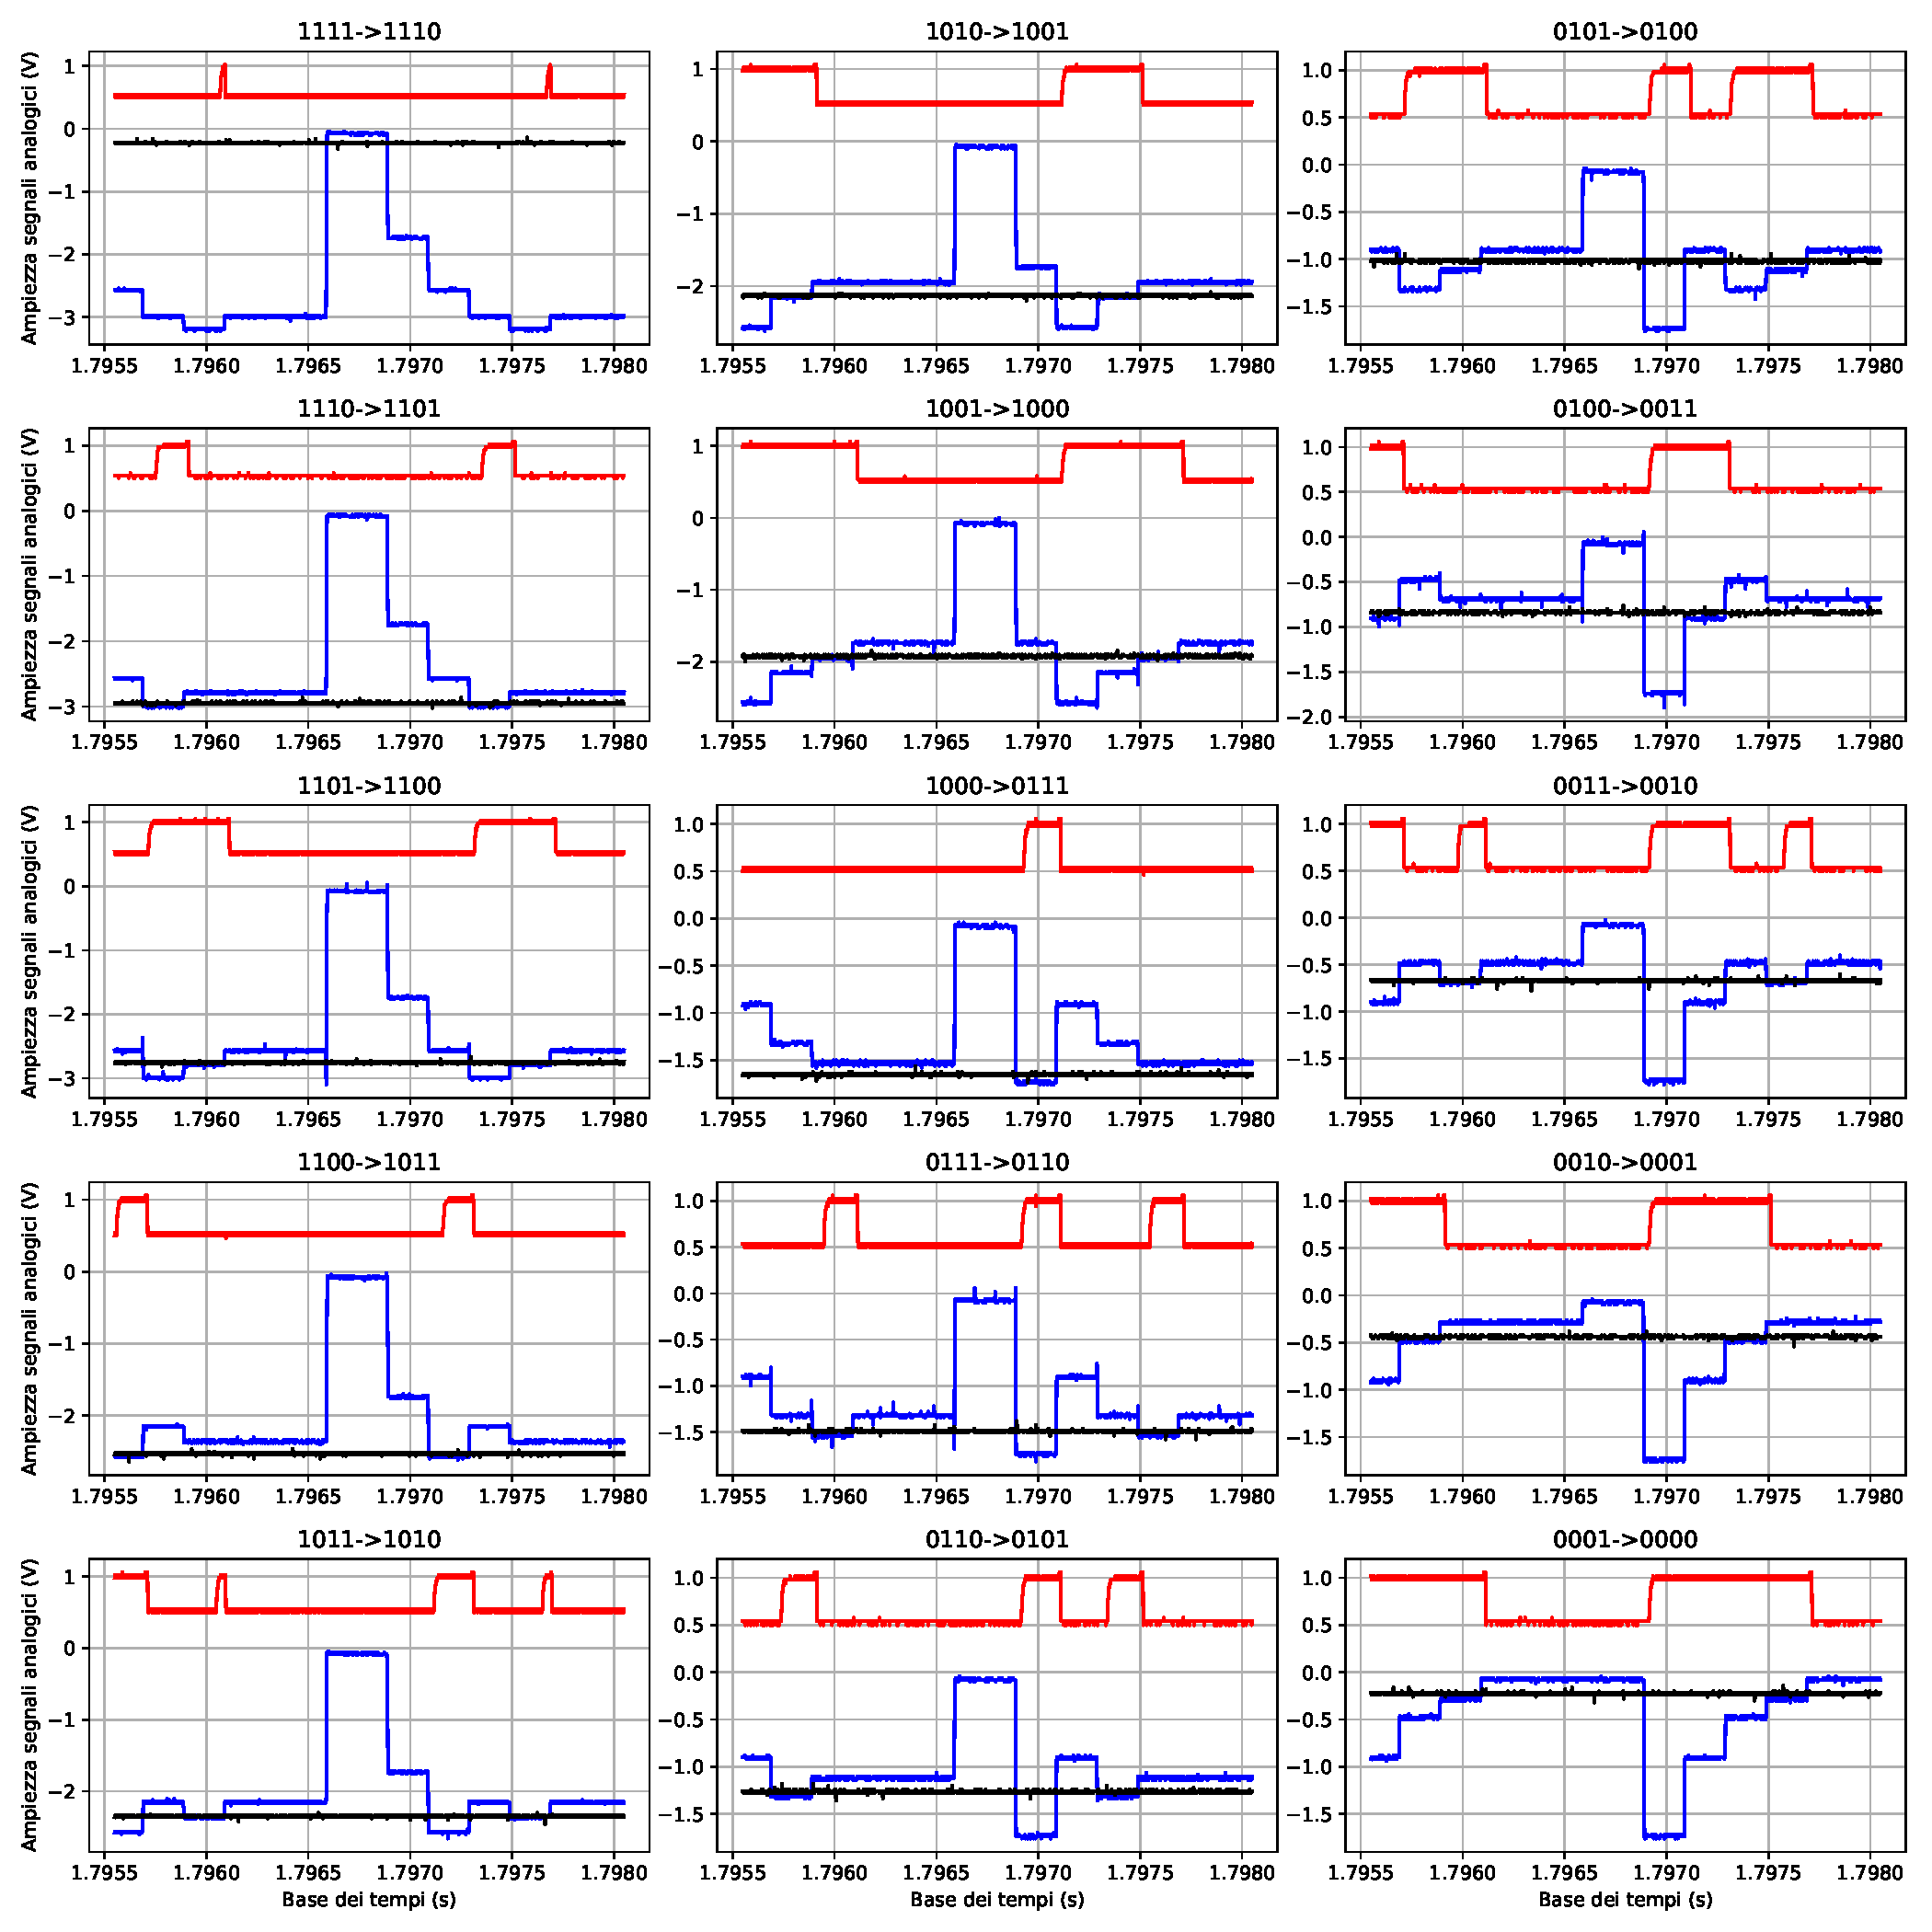
\includegraphics[trim = {30 0 50 0}, width=0.95\textwidth]{analysis/output/calibration.pdf}
\caption{Calibrazione dell'ADC. Soglia alta di transizione per ciascun bit (da 1111 a 0000). In rosso il complemento della sequenza di bit (collettore del transistor), in blu le approssimazioni successive all'uscita del DAC, in nero il segnale in ingresso}
\label{fig:BIT_high_transition_threshold}
\end{figure*}

\clearpage

%%%%%%%%%%%%%%%%%%%%%%%%%%%%%%%%%%%%%%%%%%%%%%%%%%%%%%%%%%%%%
\section{Campionamento di tensioni variabili}
Dopo aver caratterizzato il comportamento dell'ADC in regime stazionario, effettuiamo ora un test di campionamento di segnali variabili nel tempo. Dal momento che non abbiamo ancora introdotto il circuito di \textit{sample \& hold}, il campionamento di tali segnali è possibile solo sotto l'ipotesi di piccole variazioni del segnale in ingresso nella finestra temporale di conversione; come segnale di clock si imposta un'onda quadra TTL di frequenza f = 8 KHz sul generatore di funzioni. 

\begin{figure}[H]%[!ht]
\begin{center}
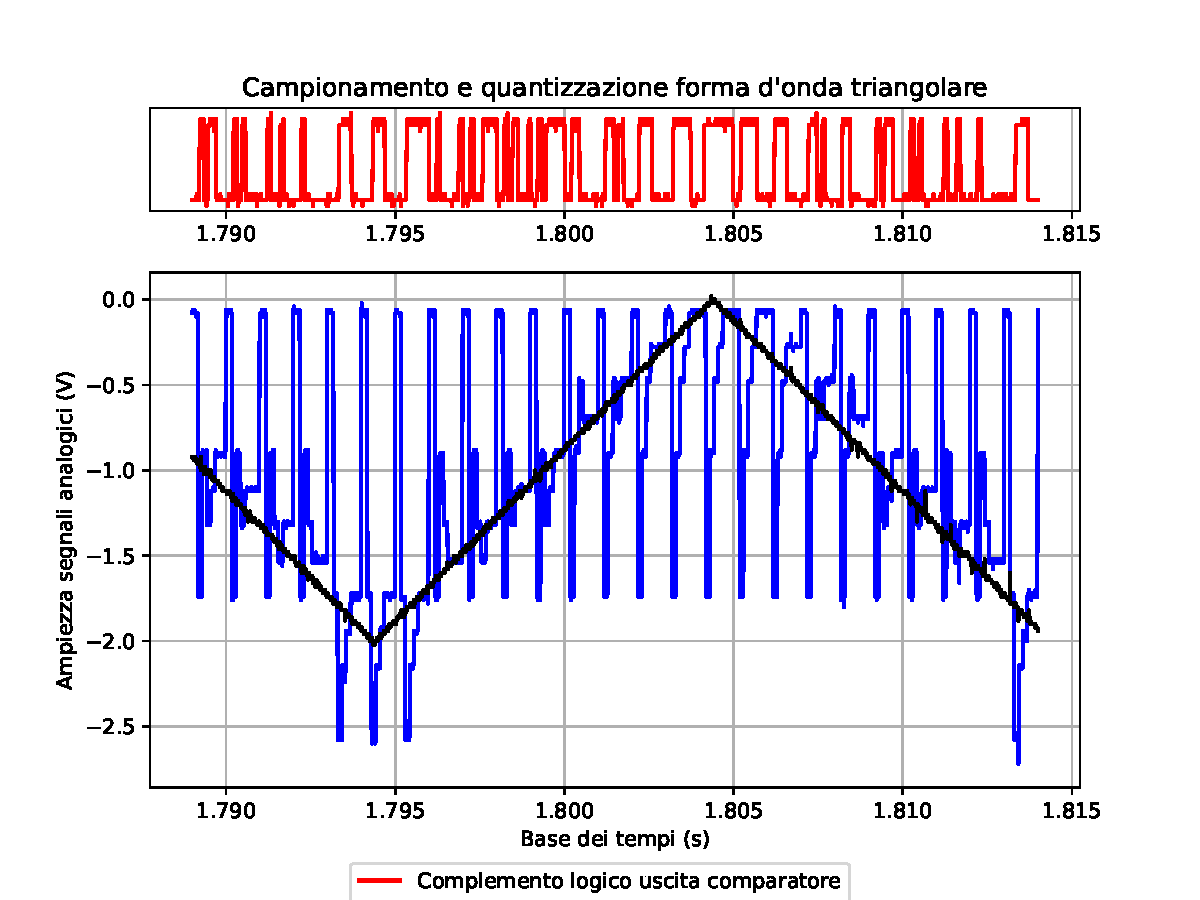
\includegraphics[trim = {0 25 0 0},clip, width=0.50\textwidth]{analysis/output/triangle_wave_aq.pdf}
\caption{Campionamento e conversione forma d'onda triangolare. In rosso il complemento logico dell'uscita del comparatore, in blu nel secondo quadrante l'uscita del DAC, in nero il segnale analogico e in blu il segnale ricostruito dall'ADC.}
\label{fig:Triangular_wave_aquisition}
\end{center}
\end{figure}

\begin{figure}[H]%[!ht]
\begin{center}
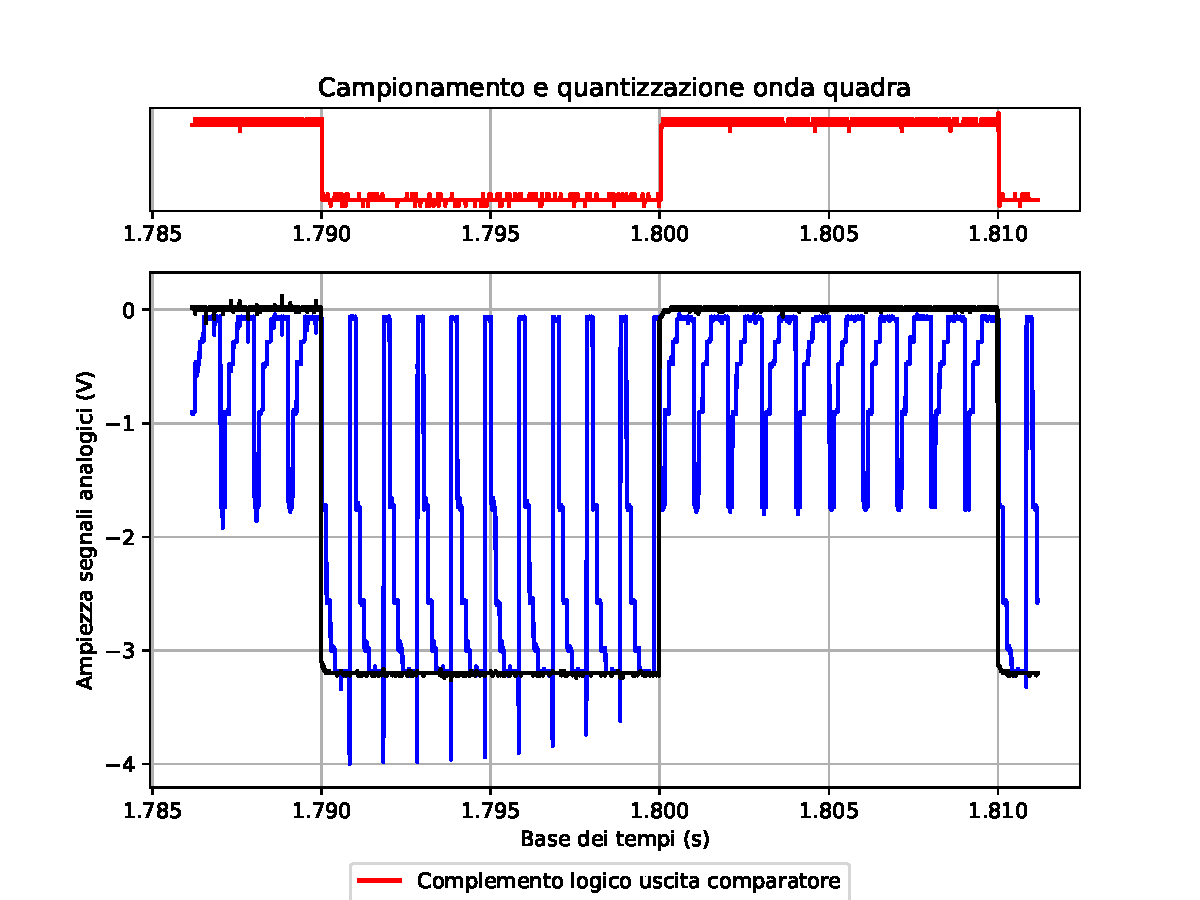
\includegraphics[trim = {0 25 0 0},clip, width=0.50\textwidth]{analysis/output/square_wave_aq.pdf}
\caption{Campionamento e conversione forma d'onda quadra. Colori come nelle figure precedenti.}
\label{fig:Square_wave_aquisition}
\end{center}
\end{figure}

Si considerino ora le figure \ref{fig:Square_wave_aquisition} e \ref{fig:Triangular_wave_aquisition}: per realizzare queste acquisizioni il canale del generatore di funzioni non occupato dal segnale di clock è stato utilizzato per generare la tensione variabile rappresentata in nero, acquisita del primo canale dell'oscilloscopio e utilizzata come riferimento per il trigger. La seconda sonda dell'oscilloscopio, corrispondente alla traccia in blu, è stata invece collegata all'uscita del DAC e mostra esattamente il processo di approssimazioni successive mentre converge al codice che più si avvicina al segnale analogico, invece in rosso è mostrato il segnale acquisito dall'oscilloscopio sul collettore del transistor di interfaccia, all'uscita del comparatore. 
La figura \ref{fig:Square_wave_aquisition} mostra l'acquisizione di un'onda quadra con livelli di tensione $V_{max}$ = 0.0 V e $V_{min}$ = -3.2 V e frequenza f = 100 Hz, mentre \ref{fig:Triangular_wave_aquisition} mostra l'acquisizione di un'onda triangolare con livelli di tensione $V_{max}$ = 0.0 V e $V_{min}$ = - 2.0 V e medesima frequenza. Nelle due figure apprezziamo in modo qualitativo il corretto funzionamento del convertitore SAR, si nota particolarmente la commutazione del MSB intorno alla metà del range dinamico del convertitore. \\

I due grafici precedenti risultano adeguati per visualizzare il processo di approssimazione, ma non consentono di confrontare agevolmente il codice ottenuto al termine del ciclo di conversione con il segnale analogico in ingresso. Per poter svolgere qualitativamente questa analisi, si utilizza nuovamente il potenziometro multigiro lineare (vedi \cite{K}) da R = (10.3 $\pm$ 0.1) K$\Omega$ per realizzare un partitore resistivo $R_A$ = (2.85 $\pm$ 0.03) K$\Omega$, $R_B$ = (7.53 $\pm$ 0.08) K$\Omega$ che attenui i segnali della logica TTL di 5 volte in tensione in modo da fornire al canale rimasto libero dell'oscilloscopio una tensione di 1 V quando l'uscita $Q_F$ del registro è allo stato alto: si tratta del segnale di conversione completata. Si imposta quindi l'oscilloscopio in modalità \textit{math} effettuando il prodotto tra questo canale e il segnale in uscita dal DAC. Si ottiene così il segnale raffigurato in blu scuro nel quadrante più in basso della figura \ref{fig:Direct_aq_waveforms}, che rappresenta il segnale logico in ingresso ricostruito dai codici prodotti dall'ADC. \\
\vspace{-10 mm}

\begin{figure}[H]%[!ht]
\begin{center}
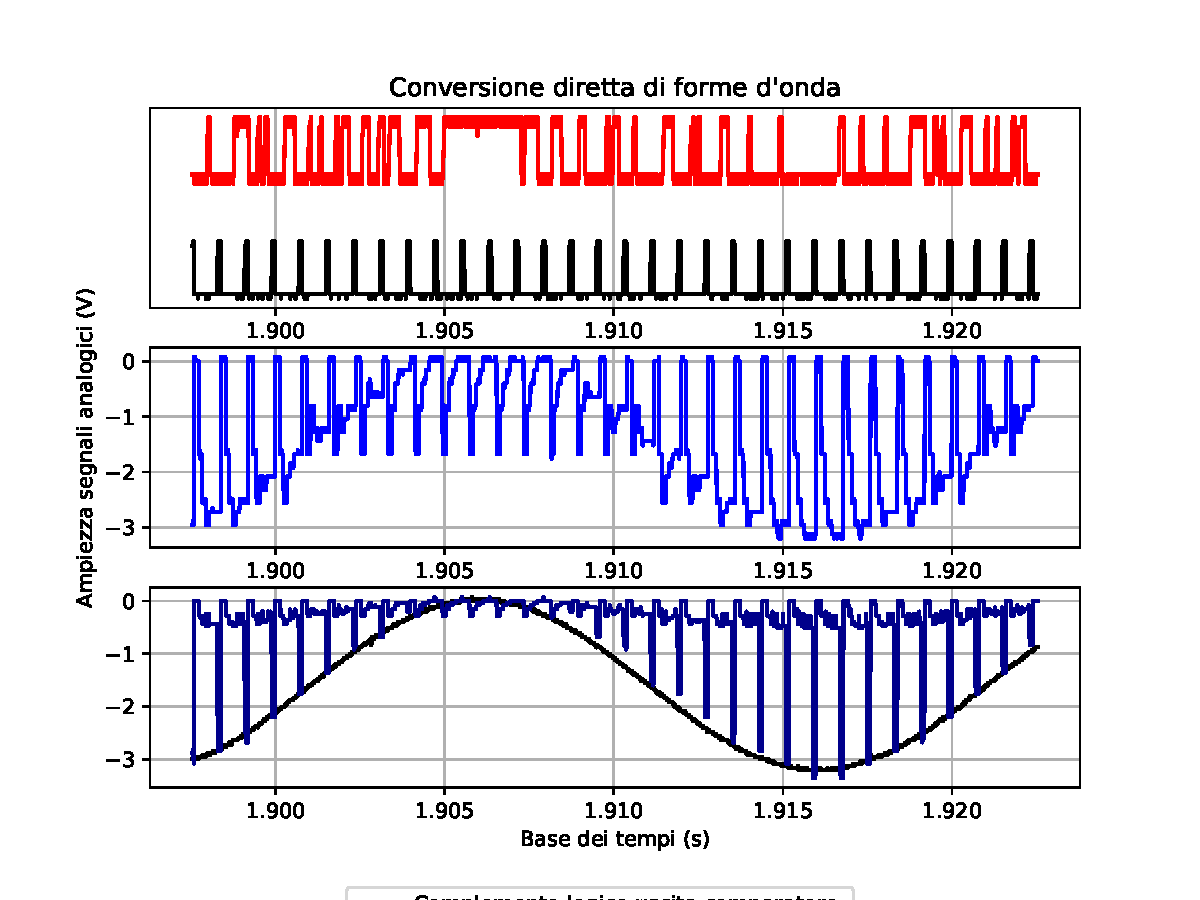
\includegraphics[trim = {0 25 0 0},clip, width=0.53\textwidth]{analysis/output/direct_aq_waveforms.pdf}
\caption{Acquisizione e conversione di una tensione sinusoidale. Colori come nelle figure precedenti, con l'aggiunta in nero nel quadrante in alto del segnale di conversione completata.}
\label{fig:Direct_aq_waveforms}
\end{center}
\end{figure}

\clearpage

\begin{figure*}[t]%[t]
\centering
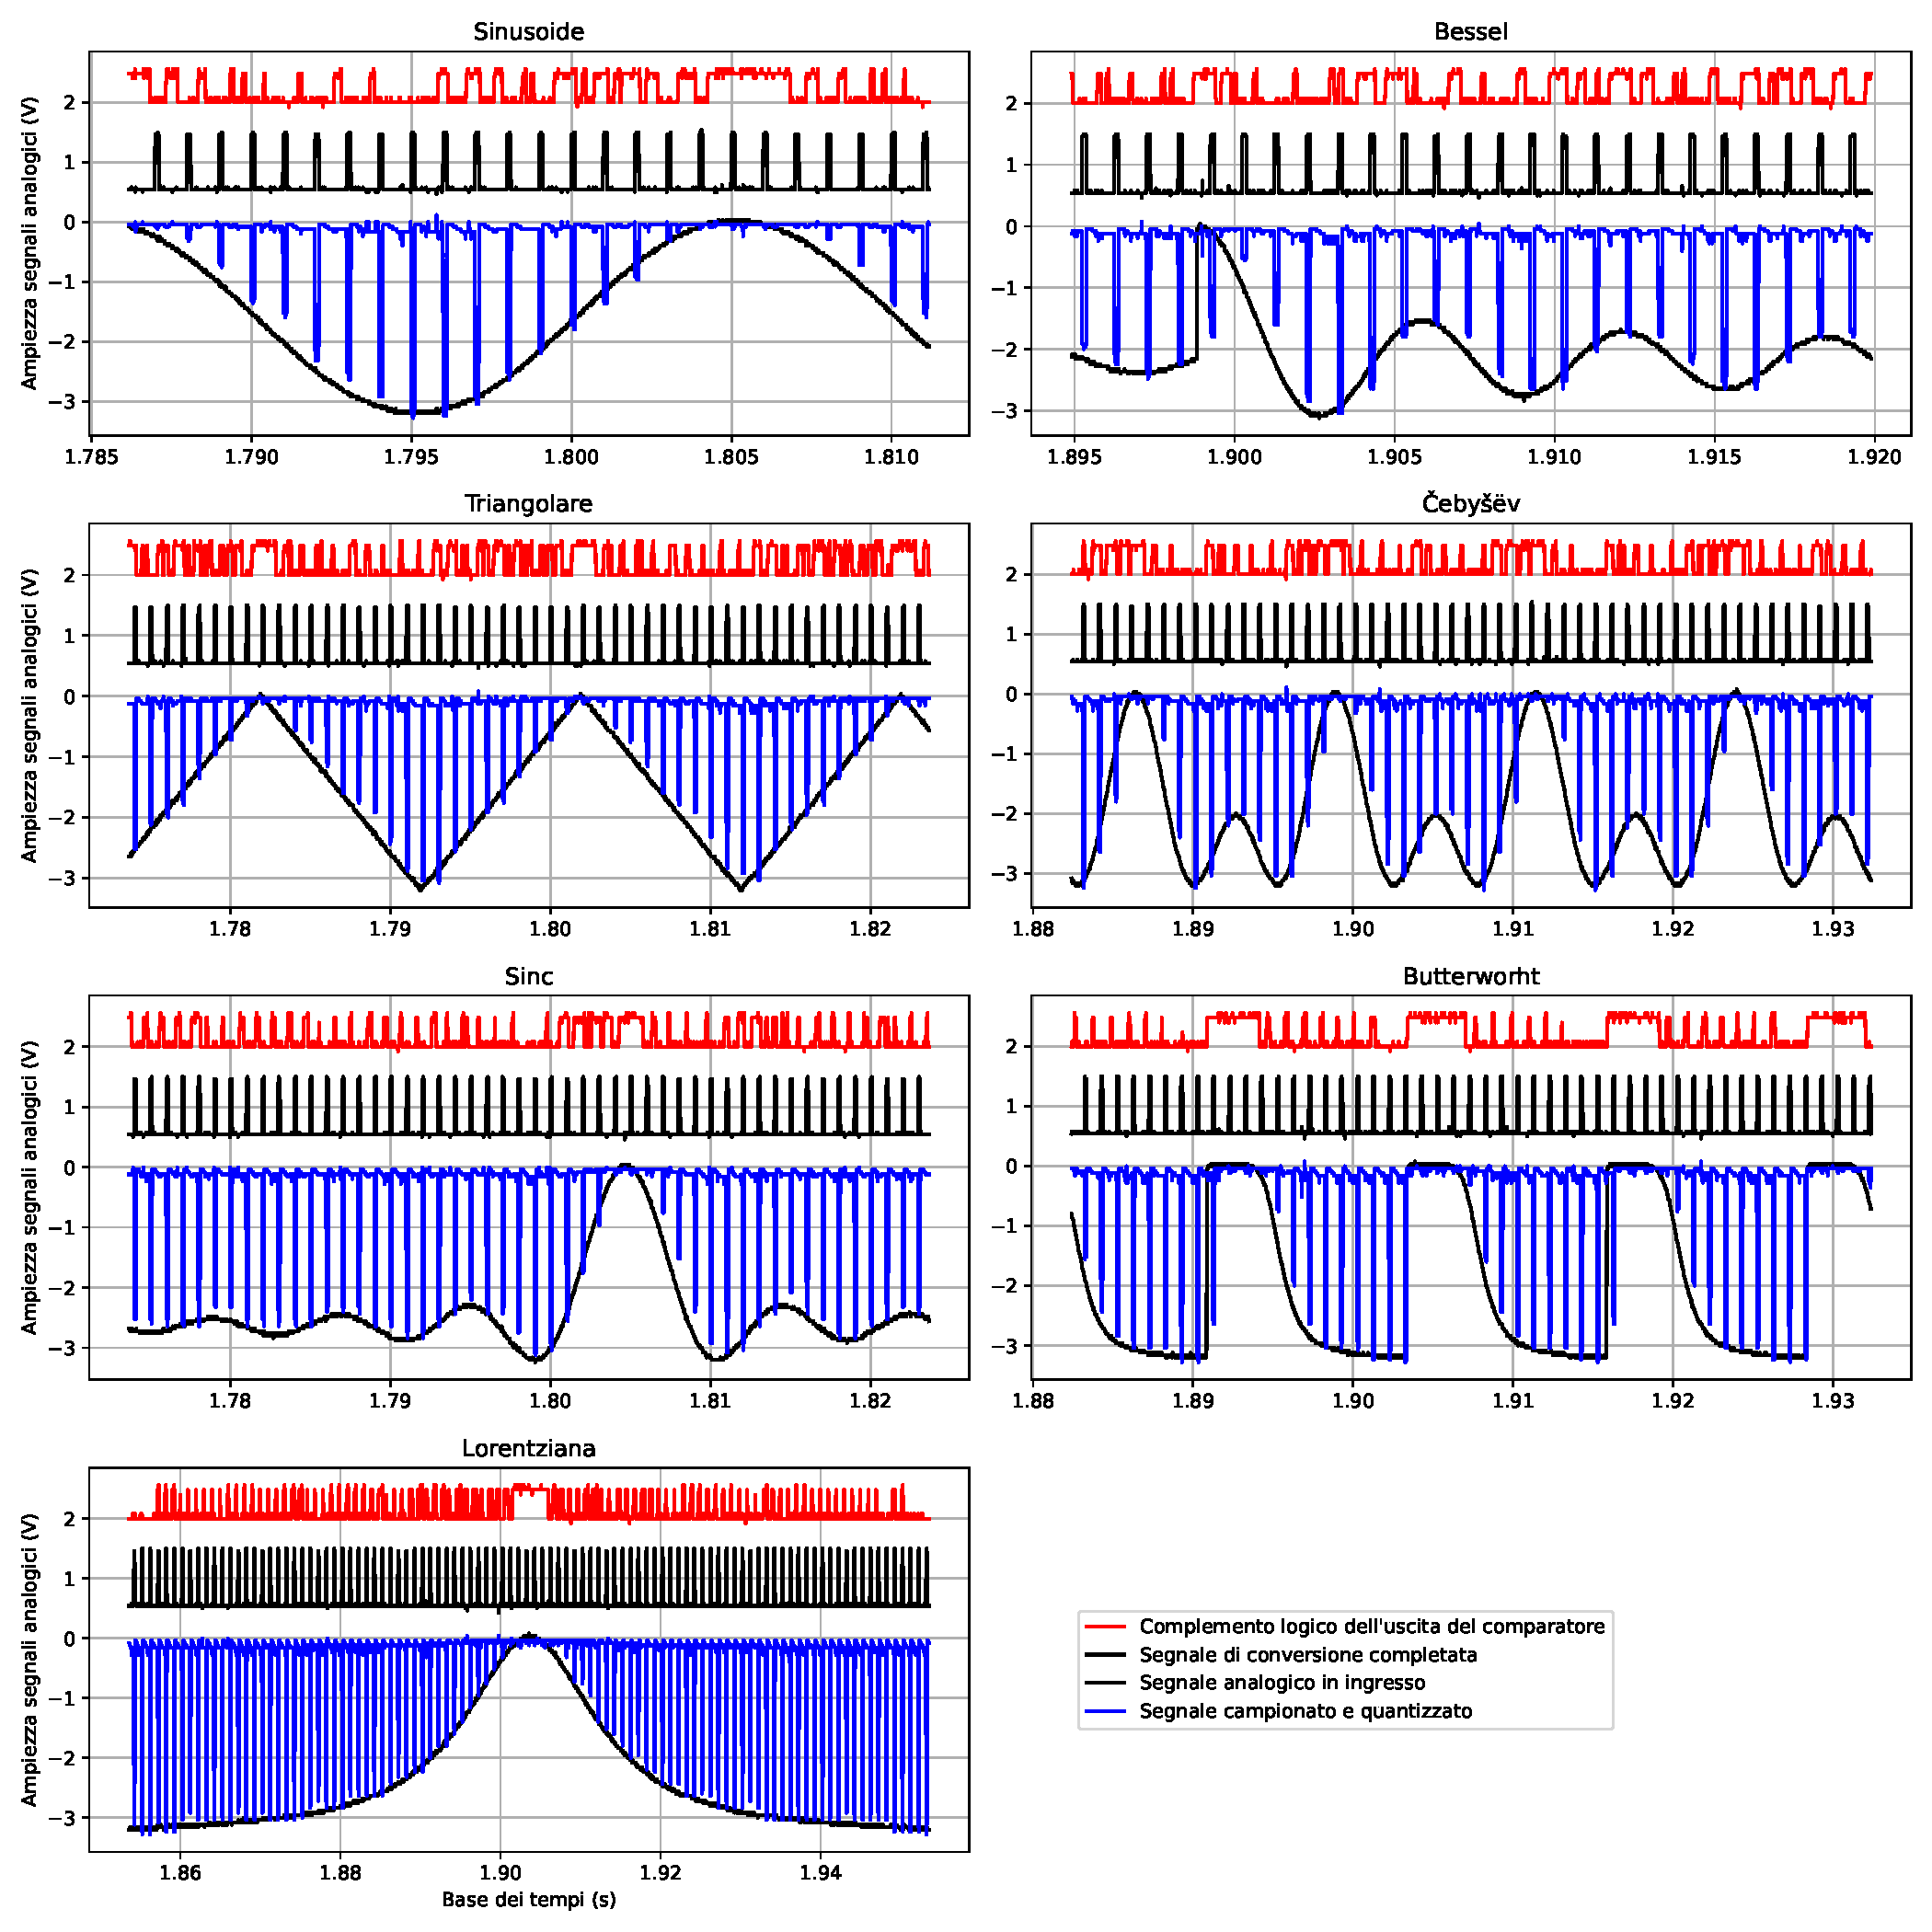
\includegraphics[trim = {30 0 50 0}, width=0.95\textwidth]{analysis/output/waveforms.pdf}
\caption{Campionamento e quantizzazione di diverse forme d'onda eseguiti con l'ADC SAR 4 bit}
\label{fig:waveforms_no_sh_scope}
\end{figure*}

\clearpage

Nella medesima figura il segnale in nero nel quadrante superiore rappresenta il segnale di conversione completata appena descritto, mentre le altre tracce sono come nelle figure \ref{fig:Triangular_wave_aquisition} e \ref{fig:Square_wave_aquisition}. Il segnale acquisito questa volta è una sinusoide oscillante tra $V_{max}$ = 0.0 V e $V_{min}$ = -3.2 V con frequenza f = 50 Hz. In figura \ref{fig:waveforms_no_sh_scope} è presentata una rassegna di forme d'onda prodotte dal generatore di funzioni nello stesso range dinamico e acquisite con l'ADC. È interessante notare che la forma d'onda ricostruita risulta sfasata indietro rispetto al segnale analogico in ingresso di un tempo pari al periodo di conversione $\tau$ = (8 bit)/$f_{clk}$ (8 bit è la lunghezza del registro di scorrimento). \\





\subsection{Circuito \textit{sample-hold}}
Finora è stato possibile eseguire il campionamento di segnali variabili nel tempo solamente sotto l'ipotesi di variazione lenta rispetto al tempo di campionamento dell'ADC. Questa ipotesi è necessaria perché il processo di approssimazioni successive dà risultati coerenti solo se durante le operazioni di confronto con l'uscita del DAC il segnale analogico in ingresso rimane pressoché costante. Per poter lavorare con segnali in ingresso più veloci, fino al limite teorico imposto dal teorema del campionamento di Nyquist-Shannon che discuteremo in seguito, si rende quindi necessaria l'introduzione di un circuito \textit{sample \& hold} che nel nostro apparato è stato realizzato con un integrato LF398. Tale componente è controllato dall'uscita $Q_F$ del registro di scorrimento: quando questo segnale digitale è alto la tensione in uscita dall'integrato insegue l'ingresso (campionamento), mentre quanto si abbassa, grazie al condensatore $C_h$, l'integrato mantiene l'uscita fissa al valore che aveva al fronte di discesa di $Q_F$. Questo fa sì che quando saranno alte le uscite del registro da $Q_A$ a $Q_E$ (operazioni di confronto) LF398 sia in modalità \textit{hold}.


\begin{figure}[H]%[!ht]
\begin{center}
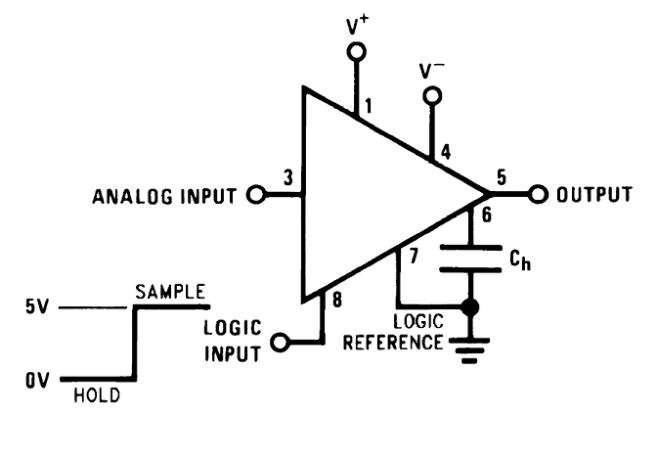
\includegraphics[width=0.35\textwidth]{sch-simulations/digital/output/lf398.png}
\caption{Schema di collegamento dell'integrato LF398 utilizzato in laboratorio per realizzare il circuito di \textit{sample and hold}, proveniente dal datasheet Texas Instruments del componente. Il valore del condensatore è $C_h$ = (10.5 $\pm$ 0.4) nF}
\label{fig:circuit_sample_and_hold}
\end{center}
\end{figure}
Per un buon funzionamento del circuito è inoltre necessario che la capacità del condensatore sia limitata in maniera tale da permettere un rapido \textit{aggancio} del segnale in ingresso nella transizione da sample a hold.
%%%%%%%%%%%%%%%%%%%%%%%%%%%%%%%%%%%%%%%%%%%%%%%%%%%%%%%%%%%%%
\section{Registrazione della conversione mediante scheda a microcontrollore}
Tutti i sistemi di acquisizione dati prevedono dopo lo stadio ADC di campionamento e quantizzazione del segnale, un'opportuna logica digitale in grado di leggere i codici prodotti dalla conversione e di di memorizzarli o visualizzarli. Tale logica oggi è frequentemente costituita da microcontrollori, dispositivi programmabili quali CPLD o FPGA o interfacce USB, PCIexpress o di altro tipo. Nel nostro caso, come abbiamo già anticipato, questa logica è costituita da un microcontrollore Atmel montato su una scheda Arduino a cui sono collegati dal pin 2 al pin 5 le uscite dei J-K a partire dal MSB. Sul pin 6 è invece collegata l'uscita $Q_F$ del registro di scorrimento, già utilizzata in precedenza poiché fornisce un segnale di conversione completata. La scheda Arduino attende che questo pin passi allo stato alto, dopodiché legge in sequenza lo stato dei pin da 2 a 5, converte in intero decimale il codice relativo e lo scrive attraverso un'interfaccia SPI su un file di testo memorizzato su una scheda di memoria. È presente un pin bistabile collegato ad un pulsante la cui pressione avvia e arresta l'acquisizione. Con il \textit{setup} appena presentato l'ADC si può considerare completo e possiamo ora effettuare nuove acquisizioni, ripetere la verifica del teorema di Nyquist con maggiore accuratezza, nonché valutare la linearità con il metodo della code density. Si considerino, ad esempio, i due grafici nelle figure \ref{fig:mcu_sine} e \ref{fig:mcu_triang} in cui si osserva rispettivamente:
\begin{itemize}
    \item l'acquisizione di una forma d'onda sinusoidale con range dinamico tra $V_{max}$ = -0.4 V e $V_{min}$ = -3.2 V e frequenza f = 50 Hz;
    \item l'acquisizione di una forma d'onda triangolare con range dinamico tra $V_{max}$ = -0.4 V e $V_{min}$ = -3.2 V e frequenza f = 5 Hz;
    \item l'acquisizione di una forma d'onda quadra con range dinamico tra $V_{max}$ = -0.4 V e $V_{min}$ = -3. V, frequenza f = 50 Hz e duty cycle del $40 \%$;
\end{itemize}

\begin{figure}[H]%[!ht]
\begin{center}
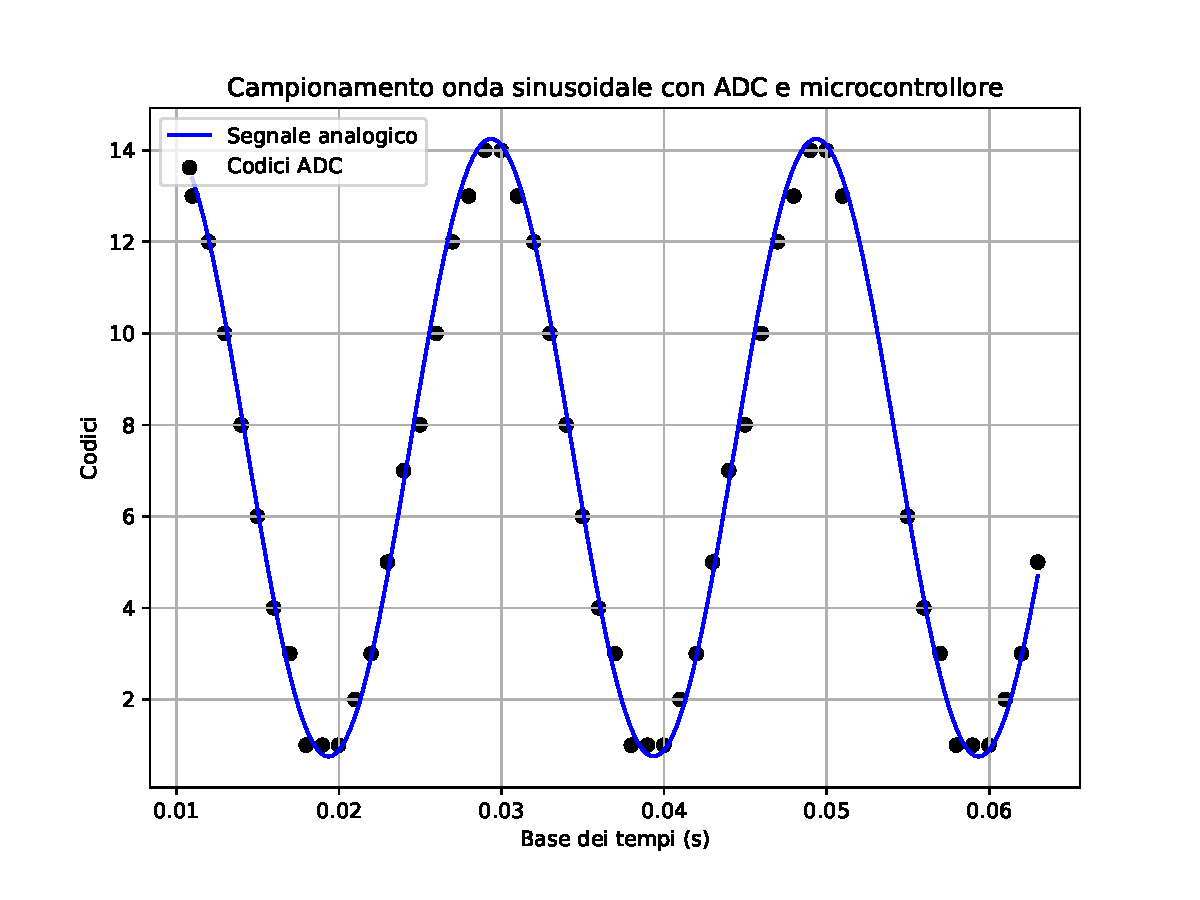
\includegraphics[trim = {0 25 0 0},clip, width=0.53\textwidth]{analysis/output/mcu_sine.pdf}
\caption{Acquisizione, con microcontrollore, di forma d'onda sinusoidale}
\label{fig:mcu_sine}
\end{center}
\end{figure}

\begin{figure}[H]%[!ht]
\begin{center}
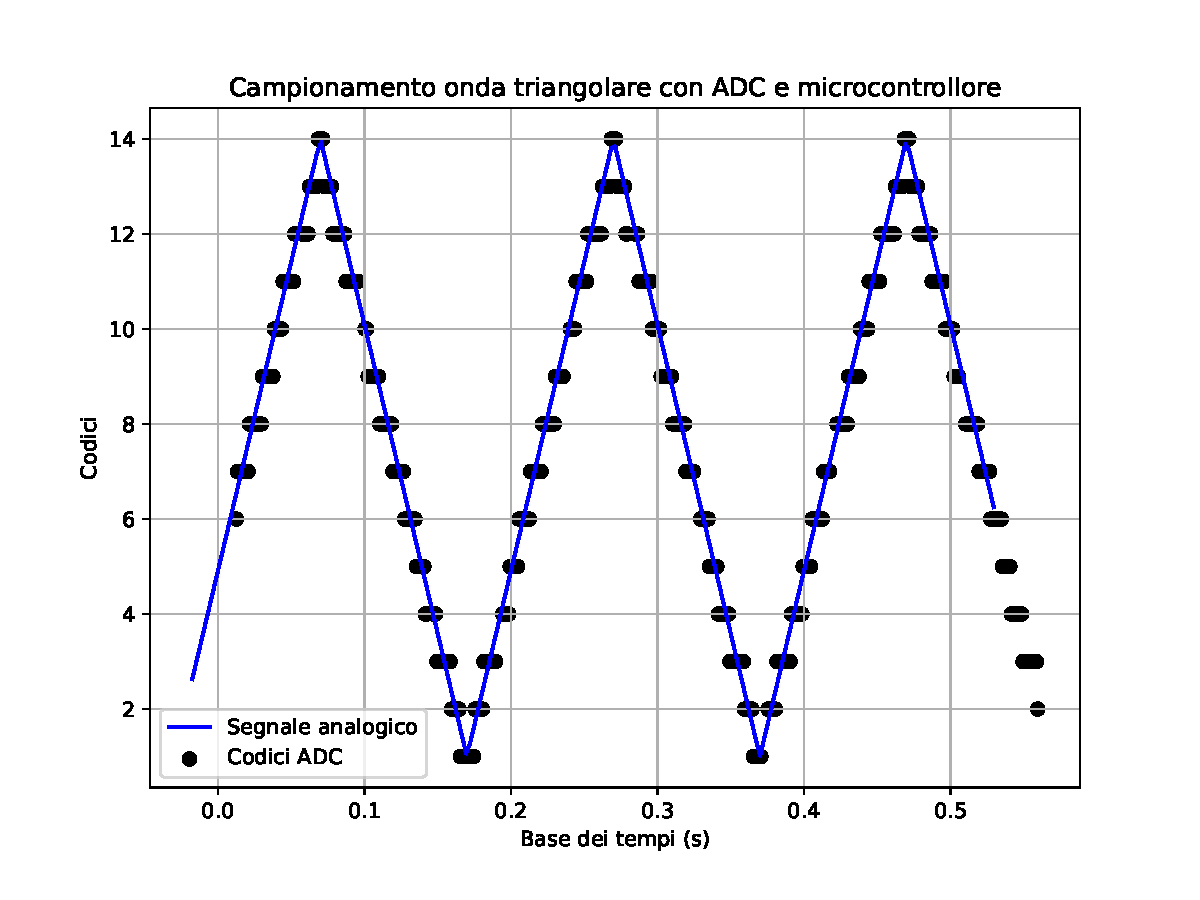
\includegraphics[trim = {0 25 0 0},clip, width=0.50\textwidth]{analysis/output/mcu_triangle.pdf}
\caption{Acquisizione, con microcontrollore, di forma d'onda triangolare}
\label{fig:mcu_triang}
\end{center}
\end{figure}

\begin{figure}[H]%[!ht]
\begin{center}
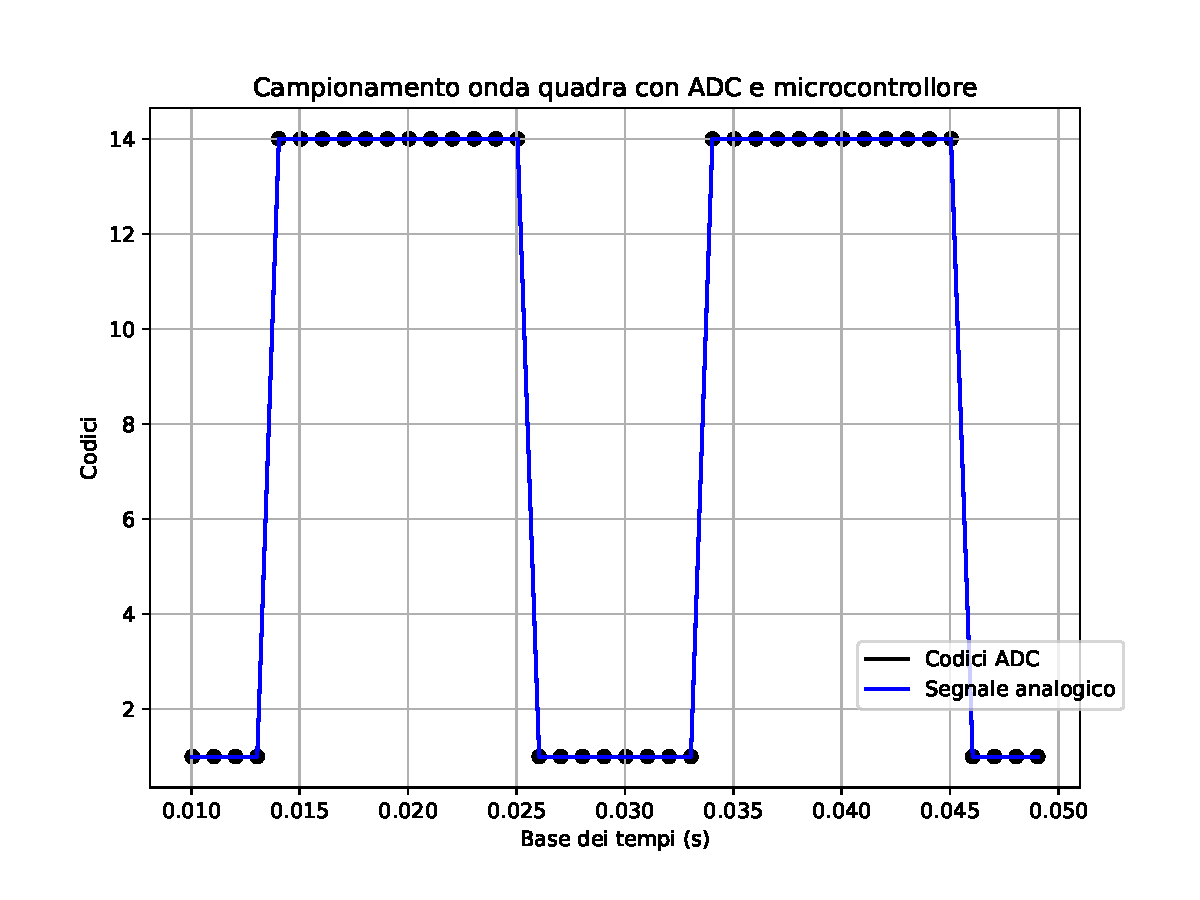
\includegraphics[trim = {0 25 0 0},clip, width=0.53\textwidth]{analysis/output/mcu_square.pdf}
\caption{Acquisizione, con microcontrollore, di forma d'onda quadra}
\label{fig:mcu_square}
\end{center}
\end{figure}



\subsection{Verifica del teorema del campionamento di Nyquist-Shannon con sample-hold e oscilloscopio}

Se consideriamo che l'operazione di conversione svolta dall'ADC trasforma il segnale analogico continuo in ingresso:
\begin{itemize}
   \item discreto nei valori, per mezzo della quantizzazione
   \item discreto nel tempo, attraverso il campionamento
\end{itemize}

Risulta necessario studiare quali siano le condizioni di tale segnale per cui è possibile ricostruirne la forma d'onda in ingresso a partire dai campioni registrati. Queste condizioni sono enunciate dal teorema del campionamento di Nyquist-Shannon: \textit{per campionare un segnale analogico a banda limitata per essere poi in grado di ricostruirlo a partire dai campioni, occorre una frequenza di campionamento $f_c$ almeno doppia rispetto al limite superiore $f_{MAX}$ dello spettro del segnale considerato nel suo dominio di frequenza.}

\begin{equation}
    f_c \ge 2 \cdot f_{MAX}
\end{equation}

A frequenze di campionamento inferiori si osserva il fenomeno dell'\textit{aliasing}, per cui si verificano delle ambiguità che portano alla ricostruzione di armoniche con frequenze diverse (inferiori) di quelle realmente presenti nel segnale in ingresso. La frequenza di queste sinusoidi di \textit{aliasing} è data dalla seguente formula:

\begin{equation}
    f_a = |f_s - f_N \cdot nint(\frac{f_s}{f_N})|
\end{equation}

con $f_N$ la \textit{folding frequency}, cioè la frequenza più alta che può essere misurata utilizzando dati campionati discretamente e $f_s$, frequenza del segnale.

%In conclusione il sottocampionamento ha due effetti:
%\begin{itemize}
%    \item Limitazione dello spettro del segnale continuo con la $f_N$, anche detta \textit{frequenza di Nyquist}
%    \item Contaminazione dello spettro del segnale digitale da alte frequenze oltre $f_N$
%\end{itemize}

%Se si conoscesse il tempo di conversione sarebbe possibile ricavare la frequenza massima che deve avere il segnale  per limitare l'errore a un quanto, ma ond'evitare di limitare eccessivamente la banda dell'ADC conviene \textit{bloccare} il segnale durante la conversione con un circuito di sample and hold, descritto nel paragrafo precendente.


In laboratorio è stata impostata una $f_{clk} = 8 kHz$ corrispondente ad una $f_c = 1 kHz$. 
Dalla \textit{figura \ref{fig:sampSH1}} alla \textit{figura \ref{fig:sampSH6}} sono riportati i segnali visualizzati sull'oscilloscopio. 
Nel primo quadrante in alto osserviamo il segnale logico di pilotaggio del \textit{sample} \& \textit{hold} (campionamento al livello alto, mantenimento al livello basso), nel secondo quadrante osserviamo invece in verde l'uscita del DAC che mostra il ciclo di approssimazione del SAR, in nero osserviamo il segnale in ingresso dopo essere passato per il circuito \textit{sample} \& \textit{hold}; nell'ultimo quadrante, infine, osserviamo in blu il segnale analogico in ingresso proveniente dal generatore di funzioni, mentre in grigio, con i picchi evidenziati dai marker, il risultato della conversione che si ottiene moltiplicando l'uscita del DAC con il segnale di pilotaggio in rosso che rappresenta a tutti gli effetti un segnale di conversione completata. 

Una spezzata tratteggiata unisce i punti ricostruiti e osserviamo come al di sotto della frequenza di Nyquist costituisca una forma d'onda periodica con frequenza pari a quella del segnale in ingresso blu, mentre a frequenze superiori a quelle di Nyquist si verifichi il fenomeno dell'\textit{aliasing}, vedere figura \ref{fig:sampSH6} in particolare).

Queste osservazioni qualitative si possono per il momento considerare soddisfacenti per la verifica del teorema di Nyquist-Shannon; nei prossimi paragrafi la verifica verrà ripetuta in modo più accurato acquisendo i campioni con la scheda Arduino.

\begin{figure}[H]%[!ht]
\begin{center}
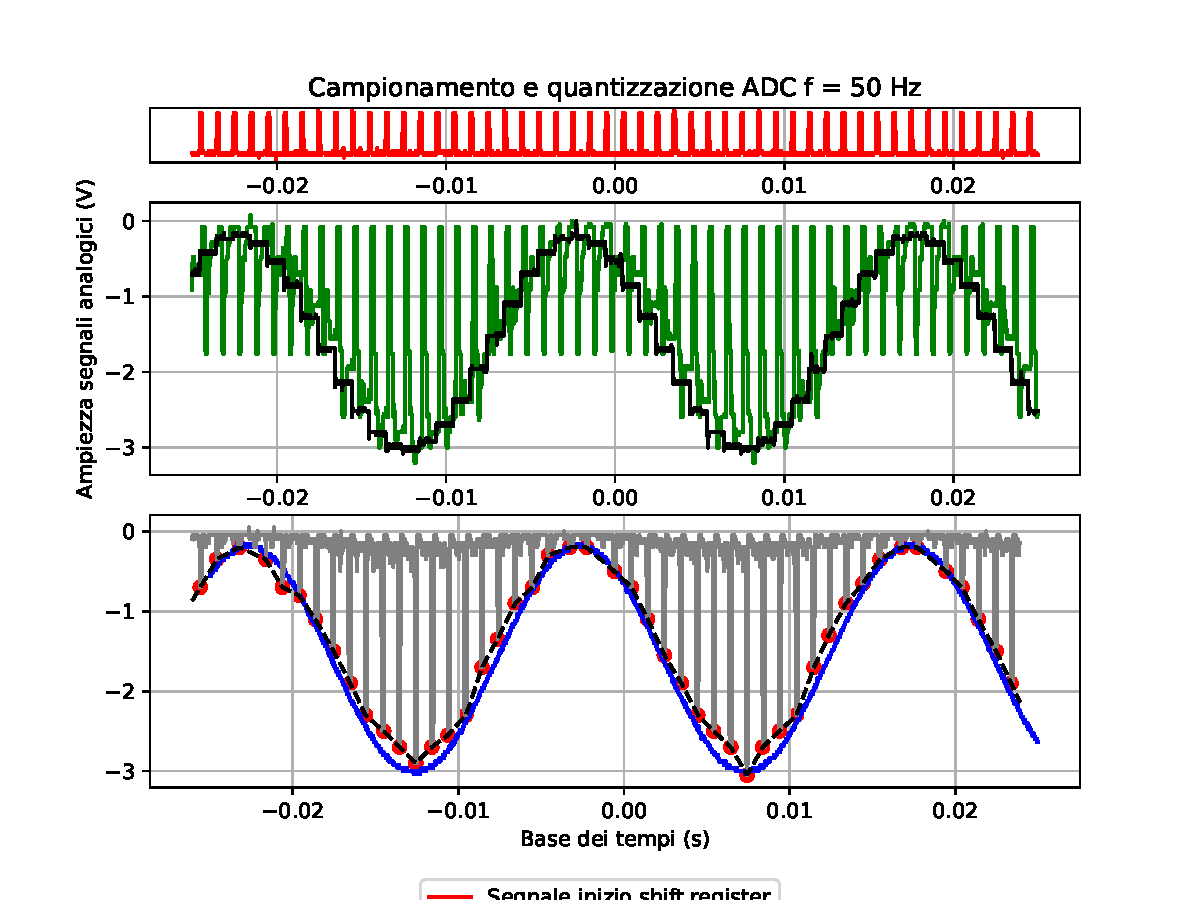
\includegraphics[ width=0.47\textwidth]{analysis/output/campionamento_50Hz.pdf}

\caption{Campionamento di forma d'onda sinusoidale $f = 50 Hz$.}
\label{fig:sampSH1}
\end{center}
\end{figure}
\vspace{-10mm}
%
\begin{figure}[H]%[!ht]
\begin{center}
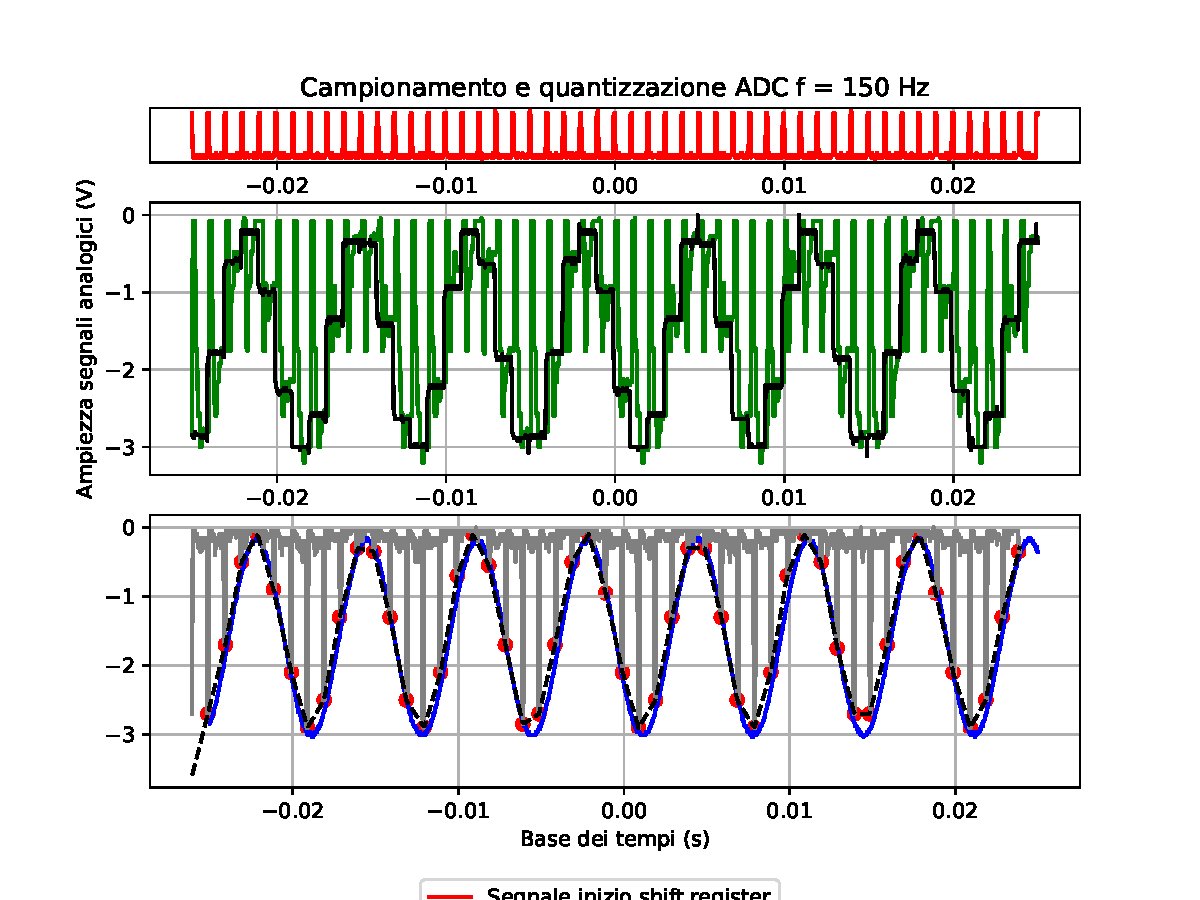
\includegraphics[trim={0 25 0 0}, clip,width=0.50\textwidth]{analysis/output/campionamento_150Hz.pdf}
\caption{Campionamento di forma d'onda sinusoidale f = 150 Hz. In rosso il segnale logico di controllo del sample-hold, in nero il segnale in uscita dal sample-hold, in verde il segnale in uscita dal DAC, il blu il segnale analogico in ingresso e in grigio il segnale ricostruito dall'ADC.}
\label{fig:sampSH2}
\end{center}
\end{figure}
\vspace{-10mm}
%
\begin{figure}[H]%[!ht]
\begin{center}
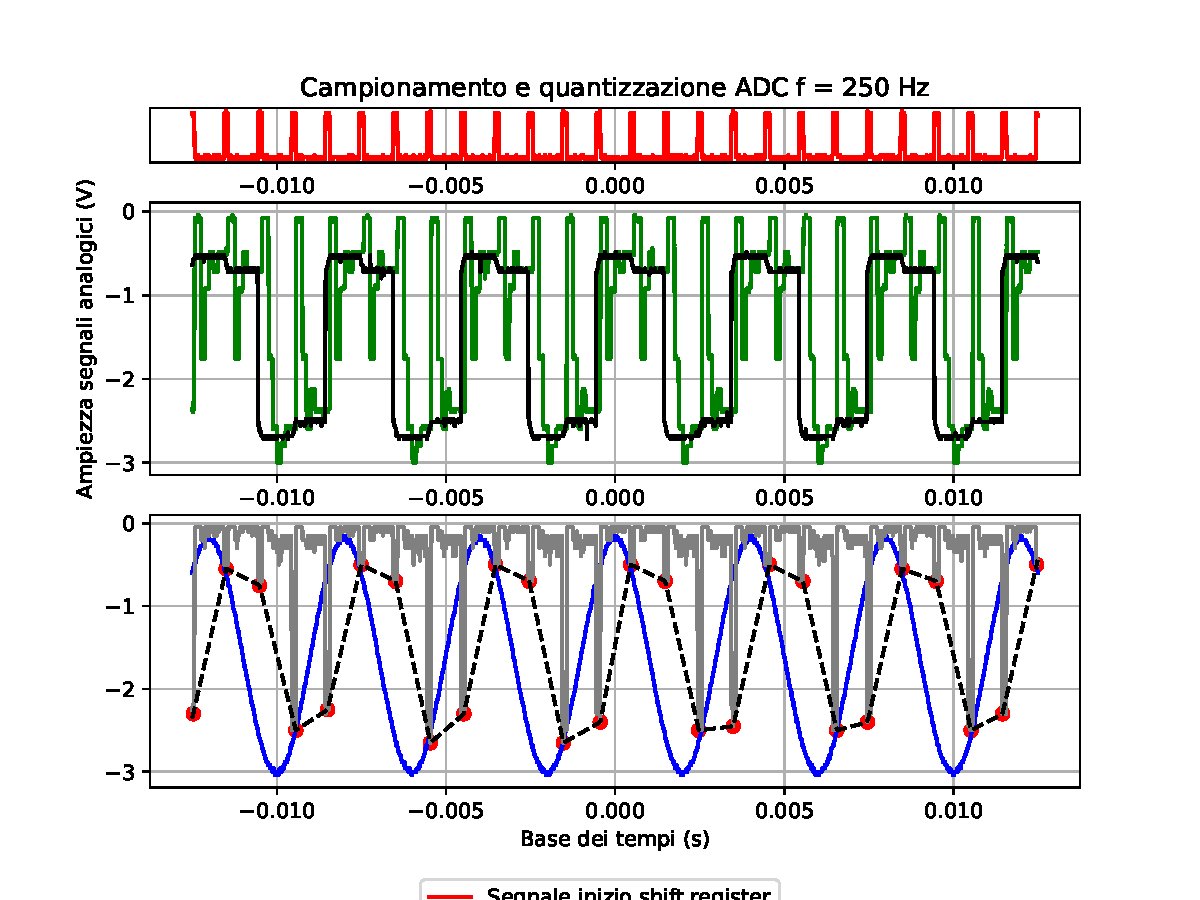
\includegraphics[trim={0 25 0 0}, clip,width=0.50\textwidth]{analysis/output/campionamento_250Hz.pdf}
\caption{Campionamento di forma d'onda sinusoidale f = 250 Hz, colori come nella figura precedente.}
\label{fig:sampSH3}
\end{center}
\end{figure}
\vspace{-10mm}
%
\begin{figure}[H]%[!ht]
\begin{center}
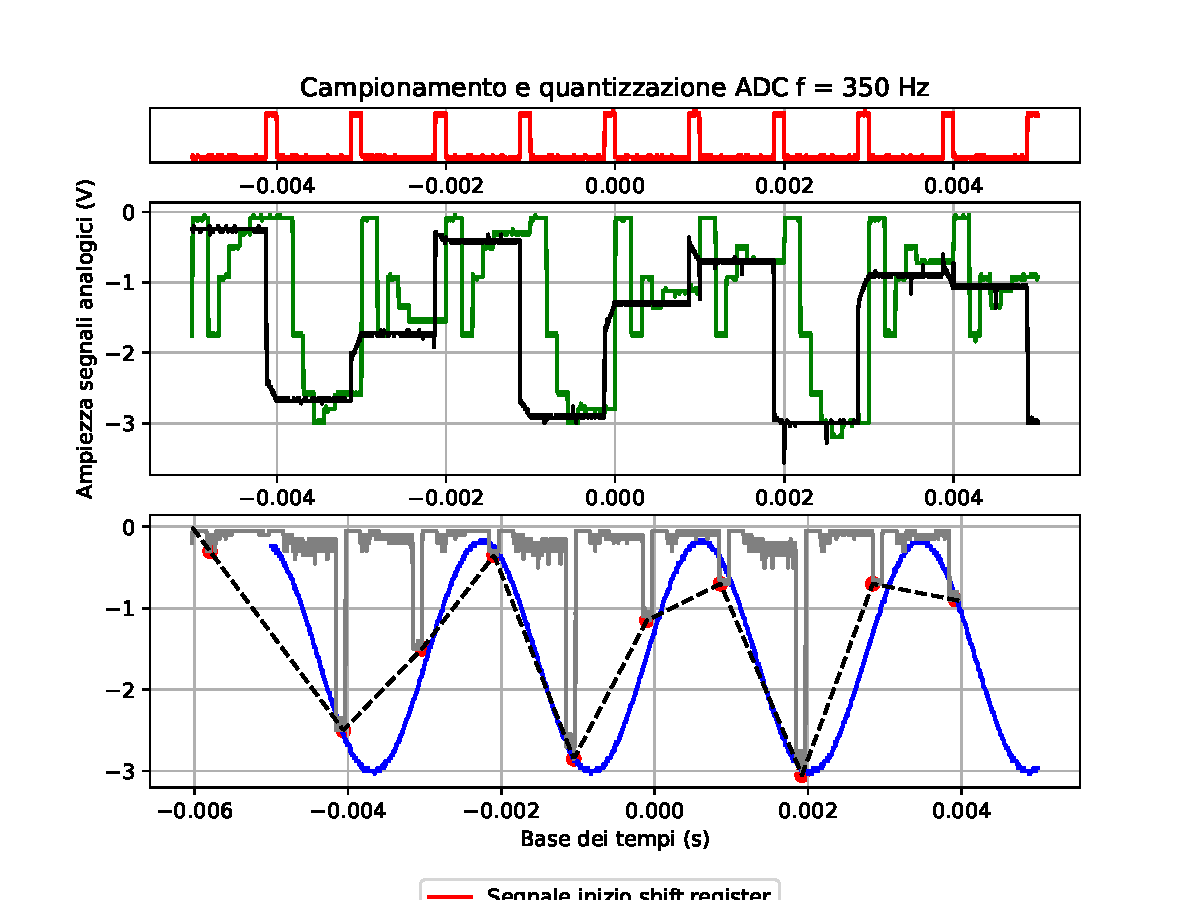
\includegraphics[trim={0 40 0 0}, clip,width=0.50\textwidth]{analysis/output/campionamento_350Hz.pdf}
\caption{Campionamento di forma d'onda sinusoidale f = 350 Hz, colori come nella figura precedente.}
\label{fig:sampSH4}
\end{center}
\end{figure}
\vspace{-10mm}
%
\begin{figure}[H]%[!ht]
\begin{center}
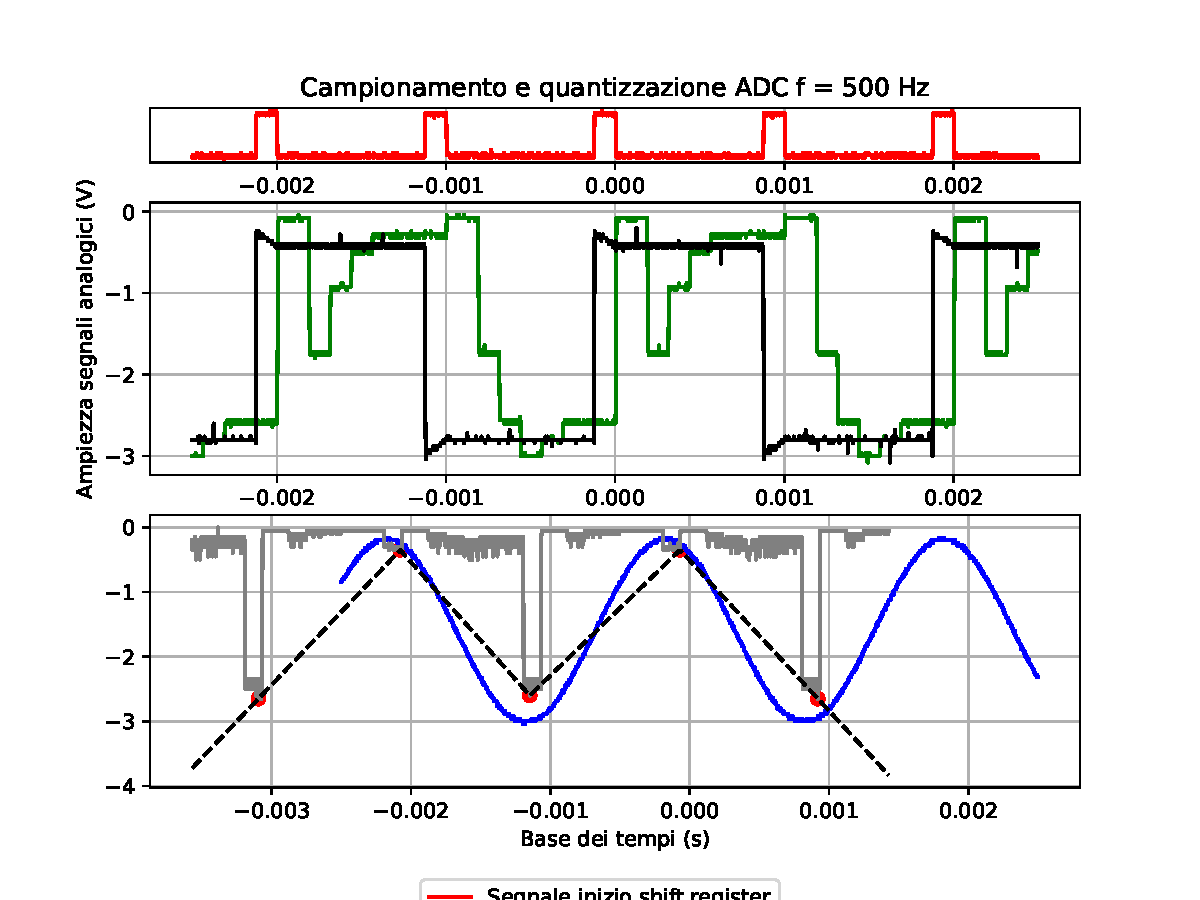
\includegraphics[trim={0 40 0 0}, clip,width=0.50\textwidth]{analysis/output/campionamento_500Hz.pdf}
\caption{Campionamento di forma d'onda sinusoidale f = 500 Hz, colori come nella figura precedente.}
\label{fig:sampSH5}
\end{center}
\end{figure}
\vspace{-10mm}
%
\begin{figure}[H]%[!ht]
\begin{center}
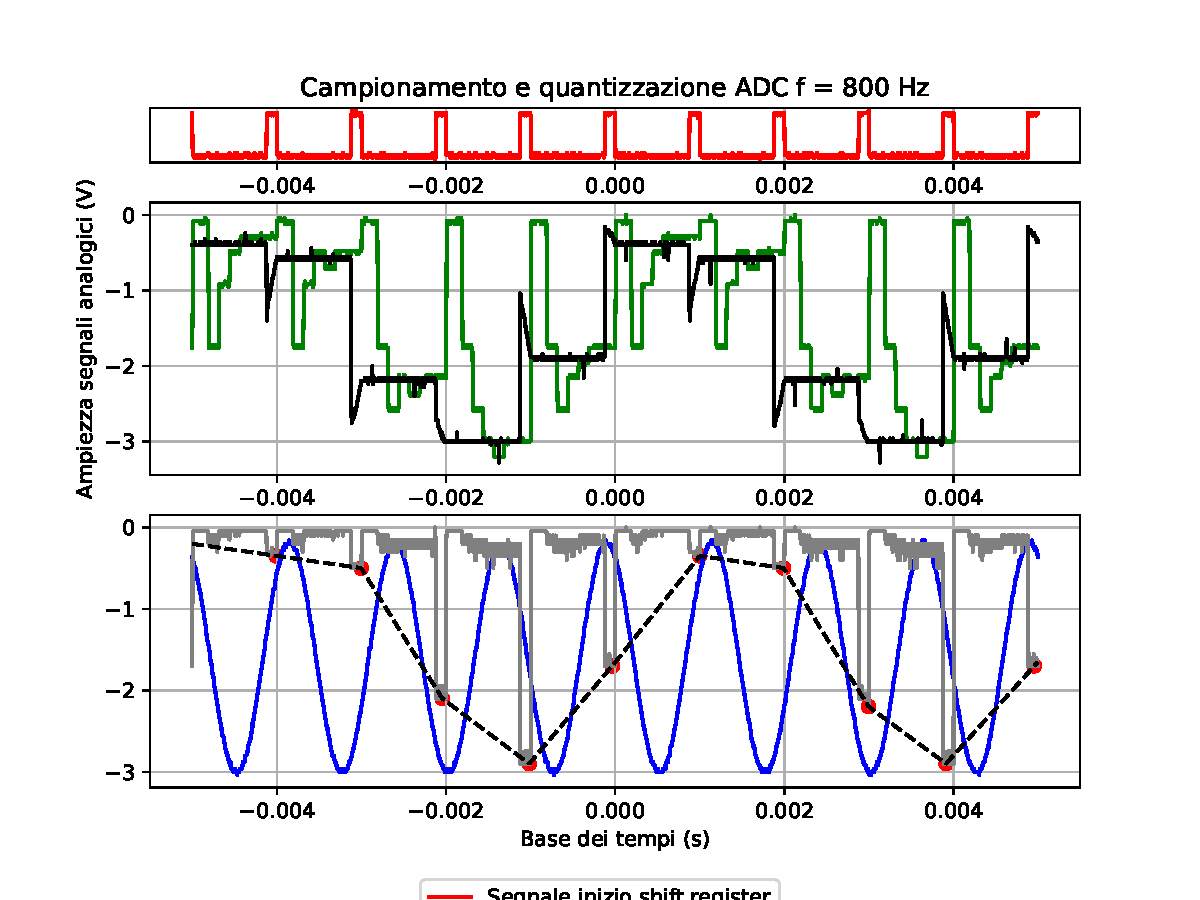
\includegraphics[trim={0 40 0 0}, clip,width=0.50\textwidth]{analysis/output/campionamento_800Hz.pdf}
\caption{Campionamento di forma d'onda sinusoidale f = 800 Hz, colori come nella figura precedente.}
\label{fig:sampSH6}
\end{center}
\end{figure}


\begin{figure*}[t]%[t]
\centering
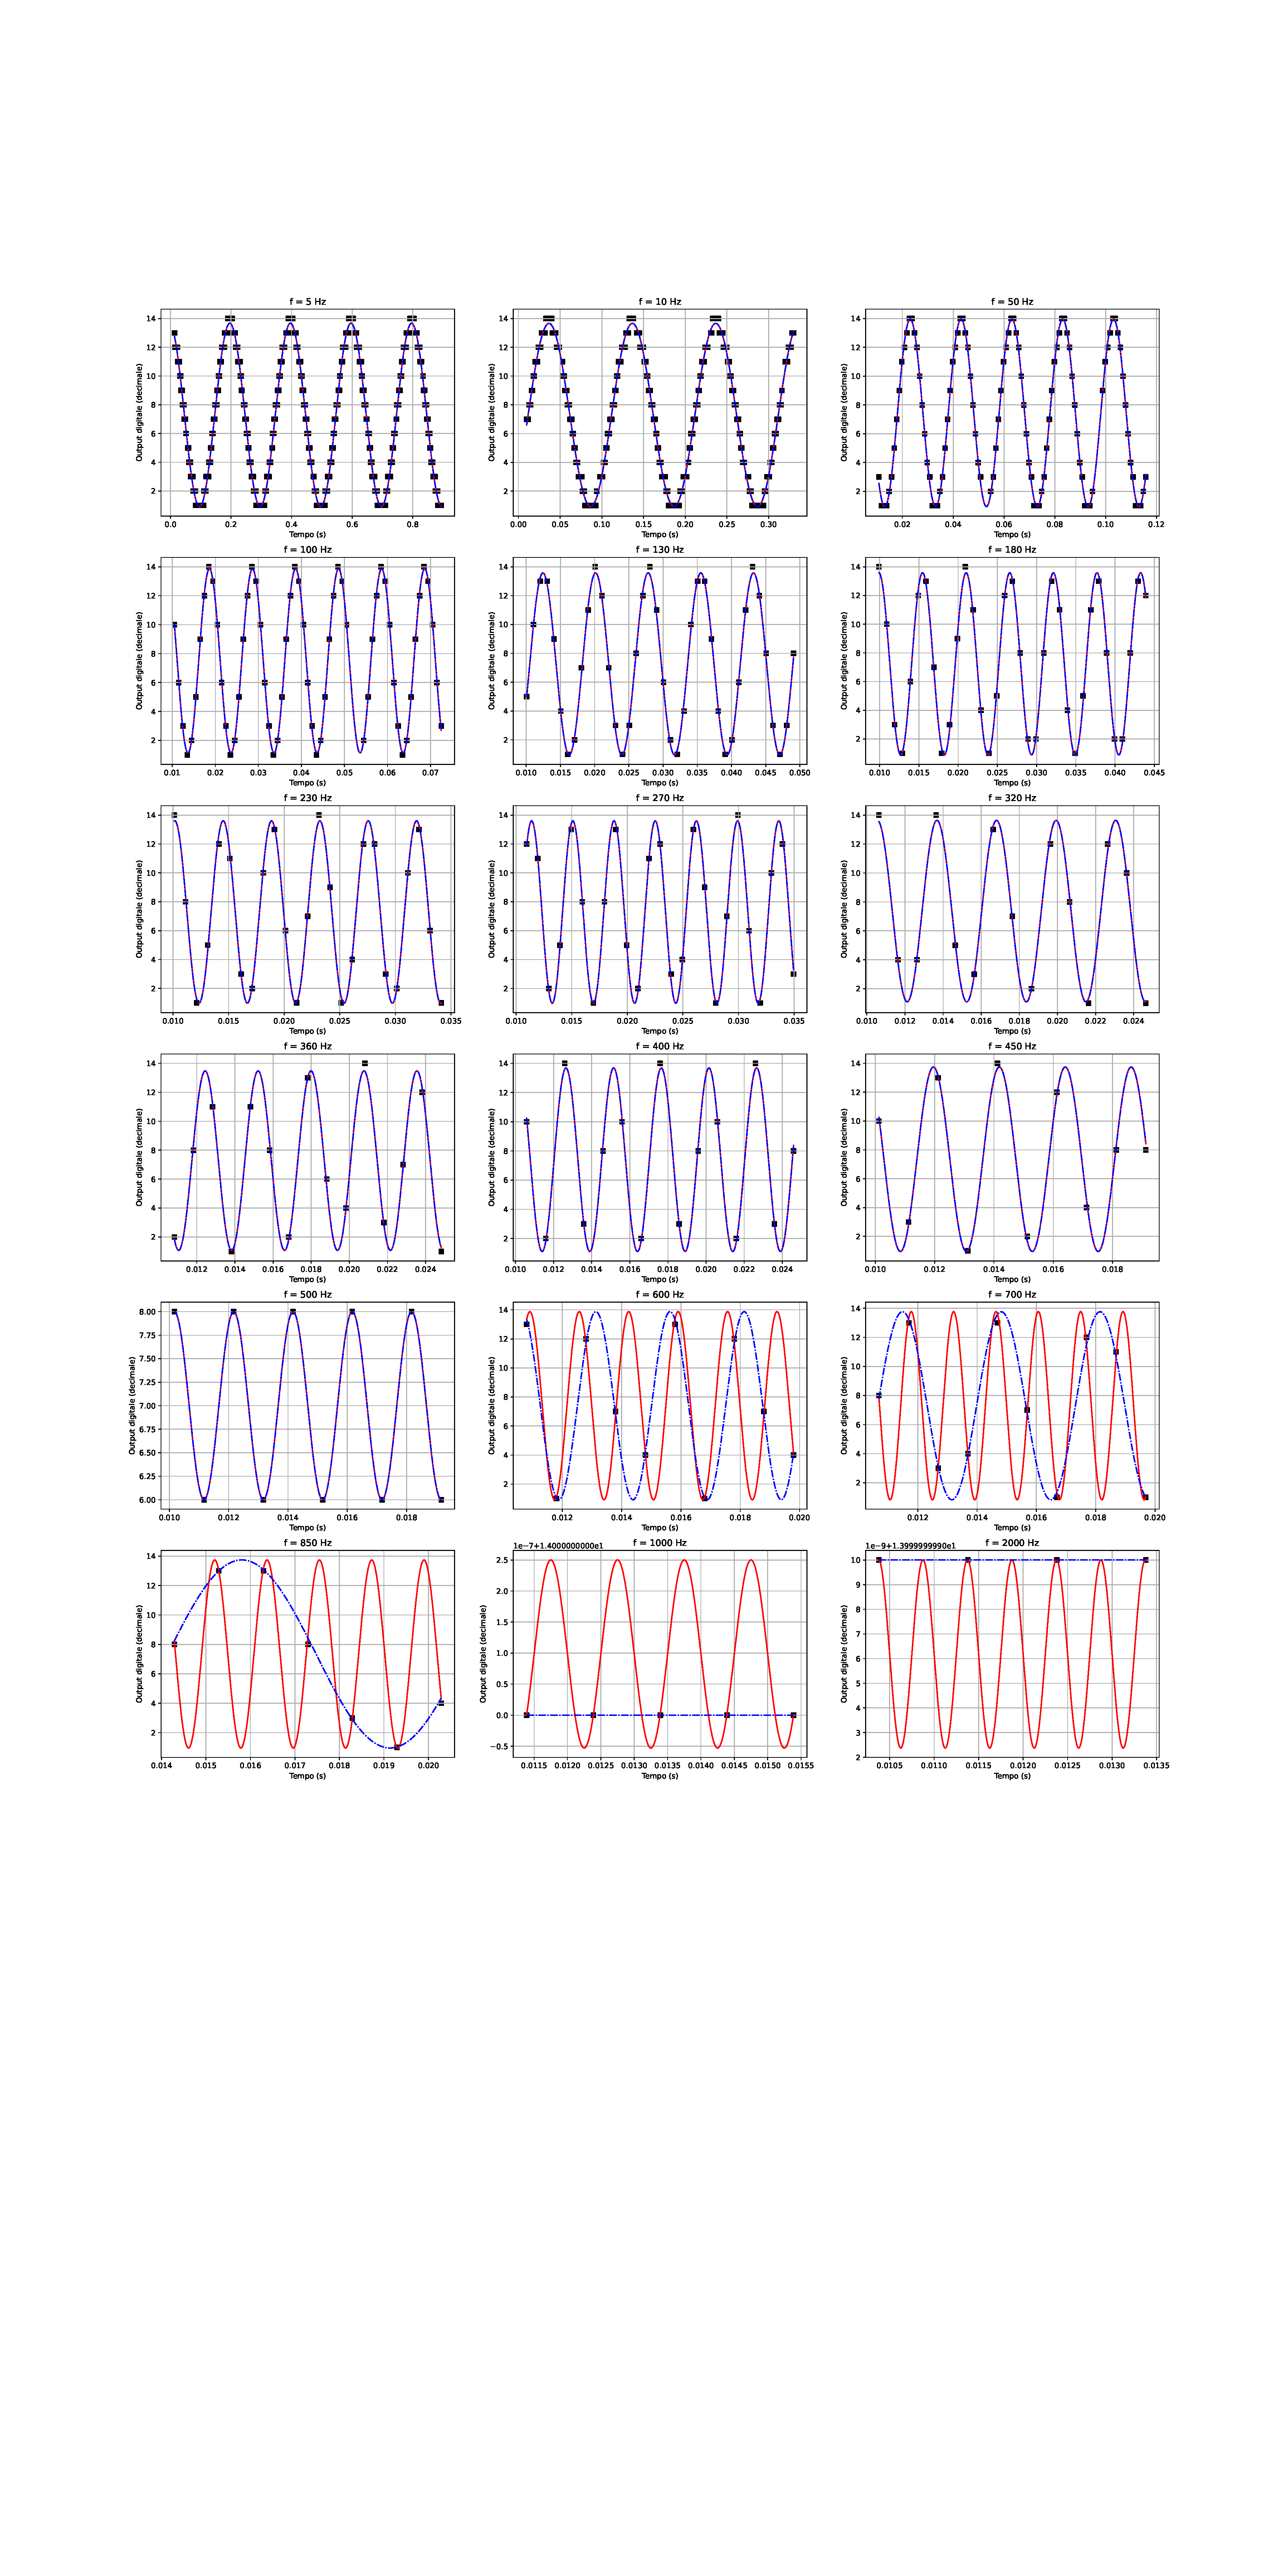
\includegraphics[trim = {150 0 0 400}, width=1.1\textwidth]{analysis/output/cumulative_nyquist_mcu.pdf}
\caption{campionamento di segnale sinusoidale con frequenze da 5 a 2000 Hz. In rosso il segnale in ingresso, in blu il fit effettuato con una sinusoide di frequenza incognita passante per i punti campionati.}
\label{fig:nyquist_mcu_cumulative}
\end{figure*}

\subsection{Verifica del teorema del campionamento di Nyquist-Shannon con \textit{sample-hold} e acquisizione con microcontrollore}

Ripetiamo ora l'analisi effettuata in precedenza sulla tesi del teorema di Nyquist-Shannon, ma in modo maggiormente quantitativo, acquisendo i campioni con la scheda a microcontrollore. Questa volta forniamo all'ingresso del \textit{sample} and \textit{hold} delle sinusoidi oscillanti tra $(-0.400 \pm 0.005)$  V e $(-3.00 \pm 0.03)$ V prodotte dal generatore di funzioni facendo variare sistematicamente la frequenza da 5 Hz a 2 KHz. Il clock è stato mantenuto ad una frequenza di 8 KHz, pertanto la frequenza di campionamento effettiva era di 1 KHz. Ci si attende quindi di essere in grado di ricostruire sinusoidi fino a 500 Hz.

I risultati sono mostrati in figura \ref{fig:nyquist_mcu_cumulative}, dove la traccia rossa rappresenta il segnale analogico in ingresso, i marker rappresentano i campioni acquisiti dalla scheda Arduino, mentre la traccia blu rappresenta la sinusoide che è stato possibile ricostruire a partire dai campioni registrati.

Nella tabella seguente è indicata per ciascuna acquisizione la frequenza nominale del segnale analogico in ingresso $f_n$, la frequenza misurata dall'oscilloscopio $f_o$, la frequenza ricostruita interpolando i campioni $f_f$ e infine la frequenza di \textit{aliasing} $f_a$ attesa con la formula presentata nel paragrafo precedente.

%%%TABLE
%\begin{table*}[hb]
%\begin{center}


%\caption{Verifica del teorema di Nyquist-Shannon con scheda a  microcontrollore}
%\label{fig:tablefn}
%\end{center}
%\end{table*}
\vspace{4 mm}
\begin{left}
\begin{tabular}{c|c|c|c}
$f_n$  &  $f_f$ & $f_o$  &   $f_a $ \\ \hline
5    &      4.997$ \pm $ 0.002 &      4.998$ \pm $ 0.002 &    5 \\
10   &      9.997$ \pm $ 0.002 &      9.998$ \pm $ 0.002  &   10 \\
50   &     49.992$ \pm $ 0.001 &     49.993$ \pm $ 0.001  &   50 \\
100  &     99.9850$ \pm $ 0.0008 &     99.9854$ \pm $ 0.0008  &  100 \\
130  &    129.981$ \pm $ 0.002 &    129.982$ \pm $ 0.002  &  130 \\
180  &    179.974$ \pm $ 0.001 &    179.975$ \pm $ 0.001 &  180 \\
230  &    229.966$ \pm $ 0.002 &    229.967$ \pm $ 0.002  &  230 \\
270  &    269.961$ \pm $ 0.002 &    269.962$ \pm $ 0.002  &  270 \\
320  &    319.954$ \pm $ 0.002 &    319.954$ \pm $ 0.002  &  320 \\
360  &    359.948$ \pm $ 0.002 &    359.949$ \pm $ 0.002 &  360 \\
400  &    399.942$ \pm $ 0.002 &    399.943$ \pm $ 0.002  &  400 \\
450  &    449.935$ \pm $ 0.002 &    449.936$ \pm $ 0.002&  450 \\
500  &  499.928$ \pm $ 0.002 &  499.928$ \pm $ 0.002  &  500 \\
600  &    399.943$ \pm $ 0.001 &    599.912$ \pm $ 0.001    &  400 \\
700  &    299.956$ \pm $ 0.001 &    699.900$ \pm $ 0.002    &  300 \\
850  &    149.978$ \pm $ 0.002 &    849.879$ \pm $ 0.002    &  150 \\
1K &     (-1.8$ \pm $ 0.9) $\cdot 10^{7}$ &  999.8587$ \pm $ 0.0002  &    0 \\
2K &     (-1.8$ \pm $ 0.9)$\cdot 10^{7}$ &   1999.7177$ \pm $ 0.0005 & 0 \\
\end{tabular}
\end{left}
\vspace{3 mm}

(Tutte le frequenze espresse in \textit{Hertz}). \\ Z di compatibilità tra $f_o$ e $f_f$: 0 fino a 500 Hz di frequenza nominale, poi (1.1, 1.8, 3.2, 41, 42) $\cdot 10^5$
\\
\vspace{5 mm}

Osserviamo immediatamente che al di sotto delle frequenza di Nyquist, pari alla metà della frequenza di campionamento, le sinusoidi vengono ricostruite correttamente e le frequenze risultano ampiamente compatibili entro il livello di significatività usuale del 5 \%. Al contrario, sopra a tale frequenza la discrepanza apprezzabile graficamente nella figura è confermata dai test di compatibilità. La frequenza su cui converge il minimizzatore che cerca di interpolare i campioni registrati in questi casi è compatibile con la frequenza di \textit{aliasing} attesa. La verifica del teorema di Nyquist può così dirsi completata con successo.


\subsection{Valutazione della linearità con metodo della \textit{code density}}
Dopo aver valutato le prestazioni dell'ADC al variare della frequenza dei segnali in ingresso, in questo paragrafo passiamo ora alla valutazione della linearità utilizzando il metodo della \textit{code density}. Si tratta di inviare all'ingresso analogico (prima del circuito \textit{sample \& hold}) un'onda triangolare che sopra uniformemente tutto il range dinamico dell'ADC e di studiare quindi le frequenze con cui si presentano i vari codici nei dati acquisiti. Naturalmente nel caso ideale ci si attenderebbe una distribuzione uniforme.

I seguenti istogrammi rappresentano le frequenze dei codici in 8 prese dati effettuate a diverse frequenze di \textit{clock} dopo aver normalizzato la media a 1. La linea rossa tratteggiata indica tale riferimento.
Affinché questa misurazione interessi tutti i codici in modo uniforme, il range di variazione del segnale di \textit{input} deve eccedere superiormente e inferiormente le soglie di \textit{clipping} dell'ADC, naturalmente il primo e l'ultimo codice non verranno quindi considerati. Per questa ragione si è scelto di utilizzare una forma d'onda triangolare con estremi -4.5 V e +0.5 V. Inoltre si è applicato uno \textit{sweep} di frequenza da 5 Hz a 50 Hz eseguito in $\Delta T$ = 35 s
con lo scopo di evitare che la scelta accidentale di frequenze multiple e sottomultiple di quella di campionamento influissero sull'uniformità dei codici acquisiti. Lo \textit{sweep} elimina anche eventuali \textit{bias} dovuti ad uno sfasamento costante tra il segnale da acquisire e il clock.
Infine i codici pari allo 0 ed al $2^n - 1$, che nel caso specifico corrisponderà a 15, sono stati esclusi dall'istogramma poiché \textit{l'overflow} e \textit{l'underflow} che si verificano agli estremi della rampa rendono privi di significato questi due \textit{bin}.

\begin{figure}[H]%[!ht]
\begin{center}

%1
\caption{$\sigma = 0.033$}
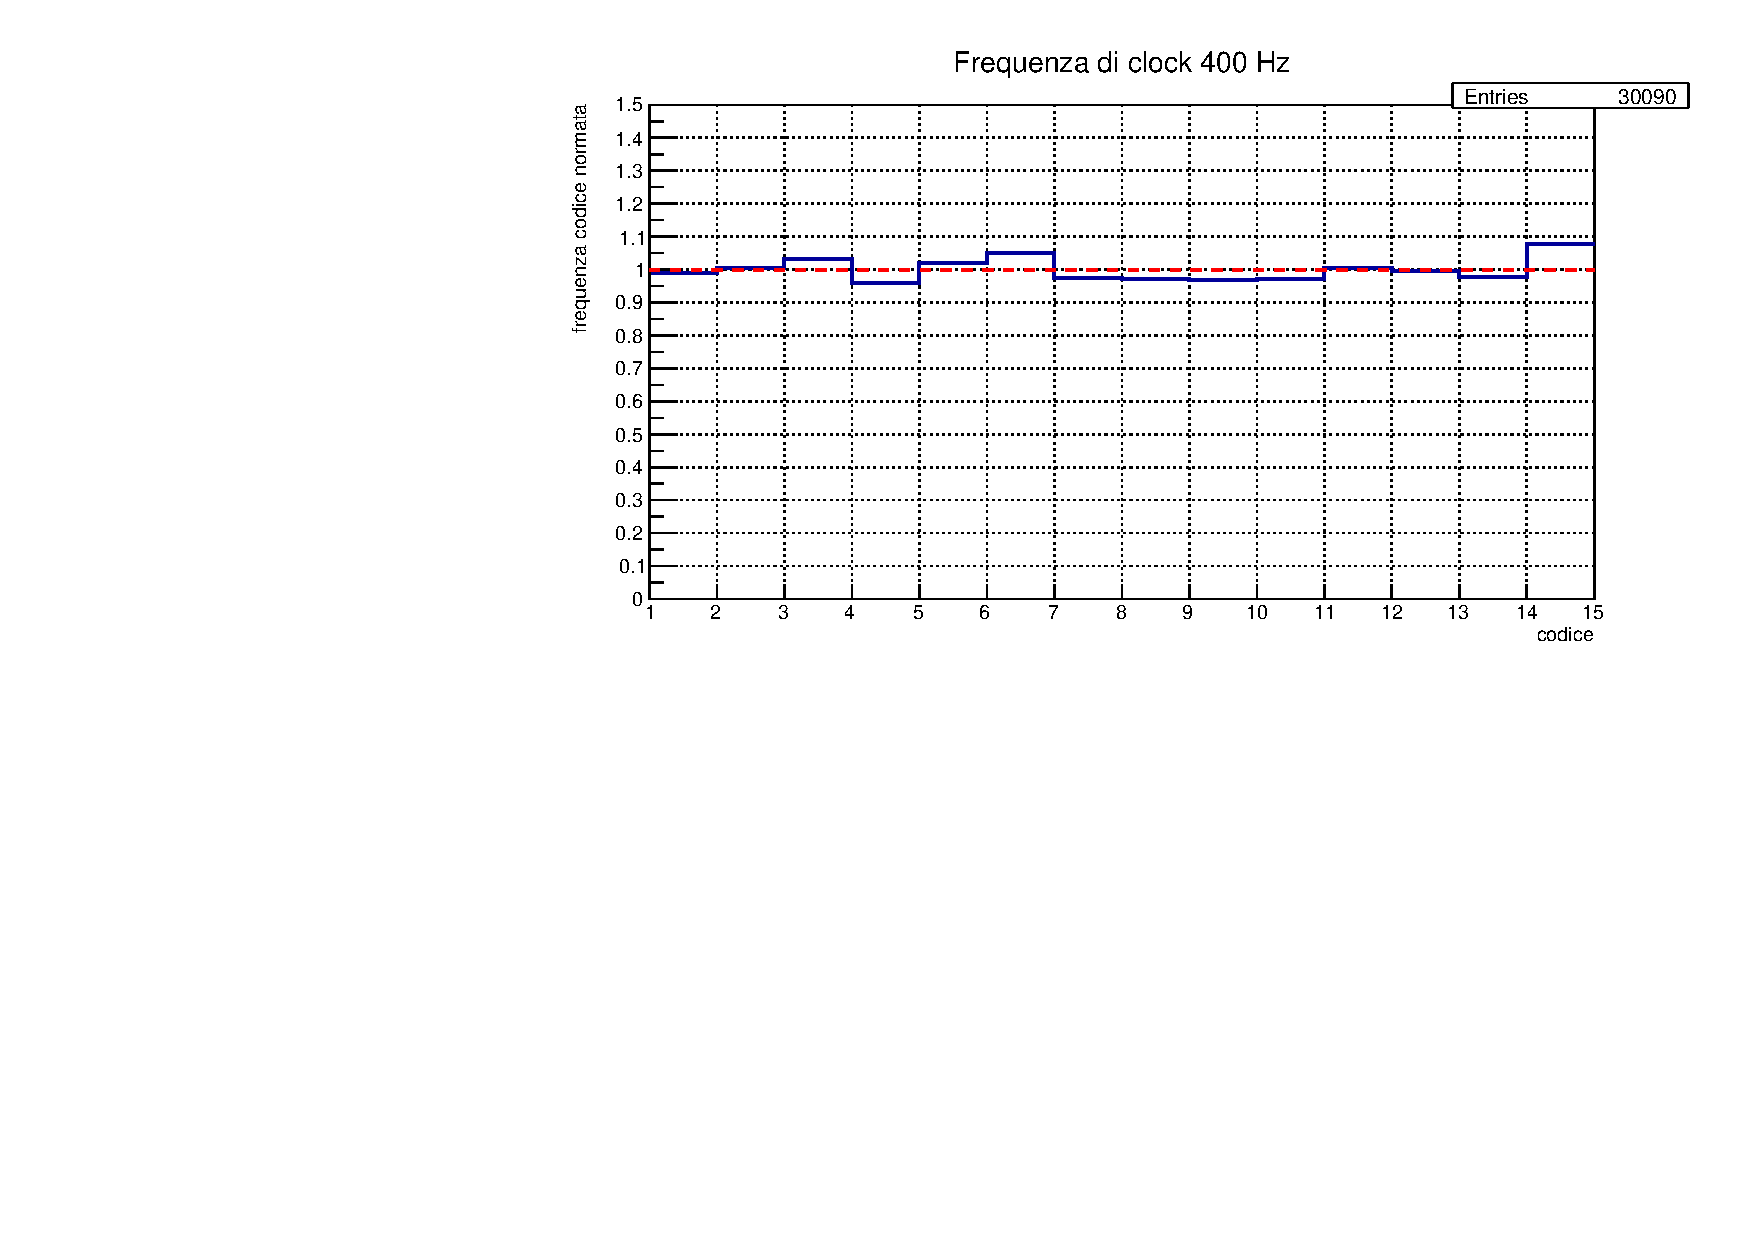
\includegraphics[width=0.48\textwidth]{analysis/output/dnl_1_400hz_bars.pdf}
\label{fig:graph_dnl_400_hz}
%2
\caption{$\sigma = 0.031$}
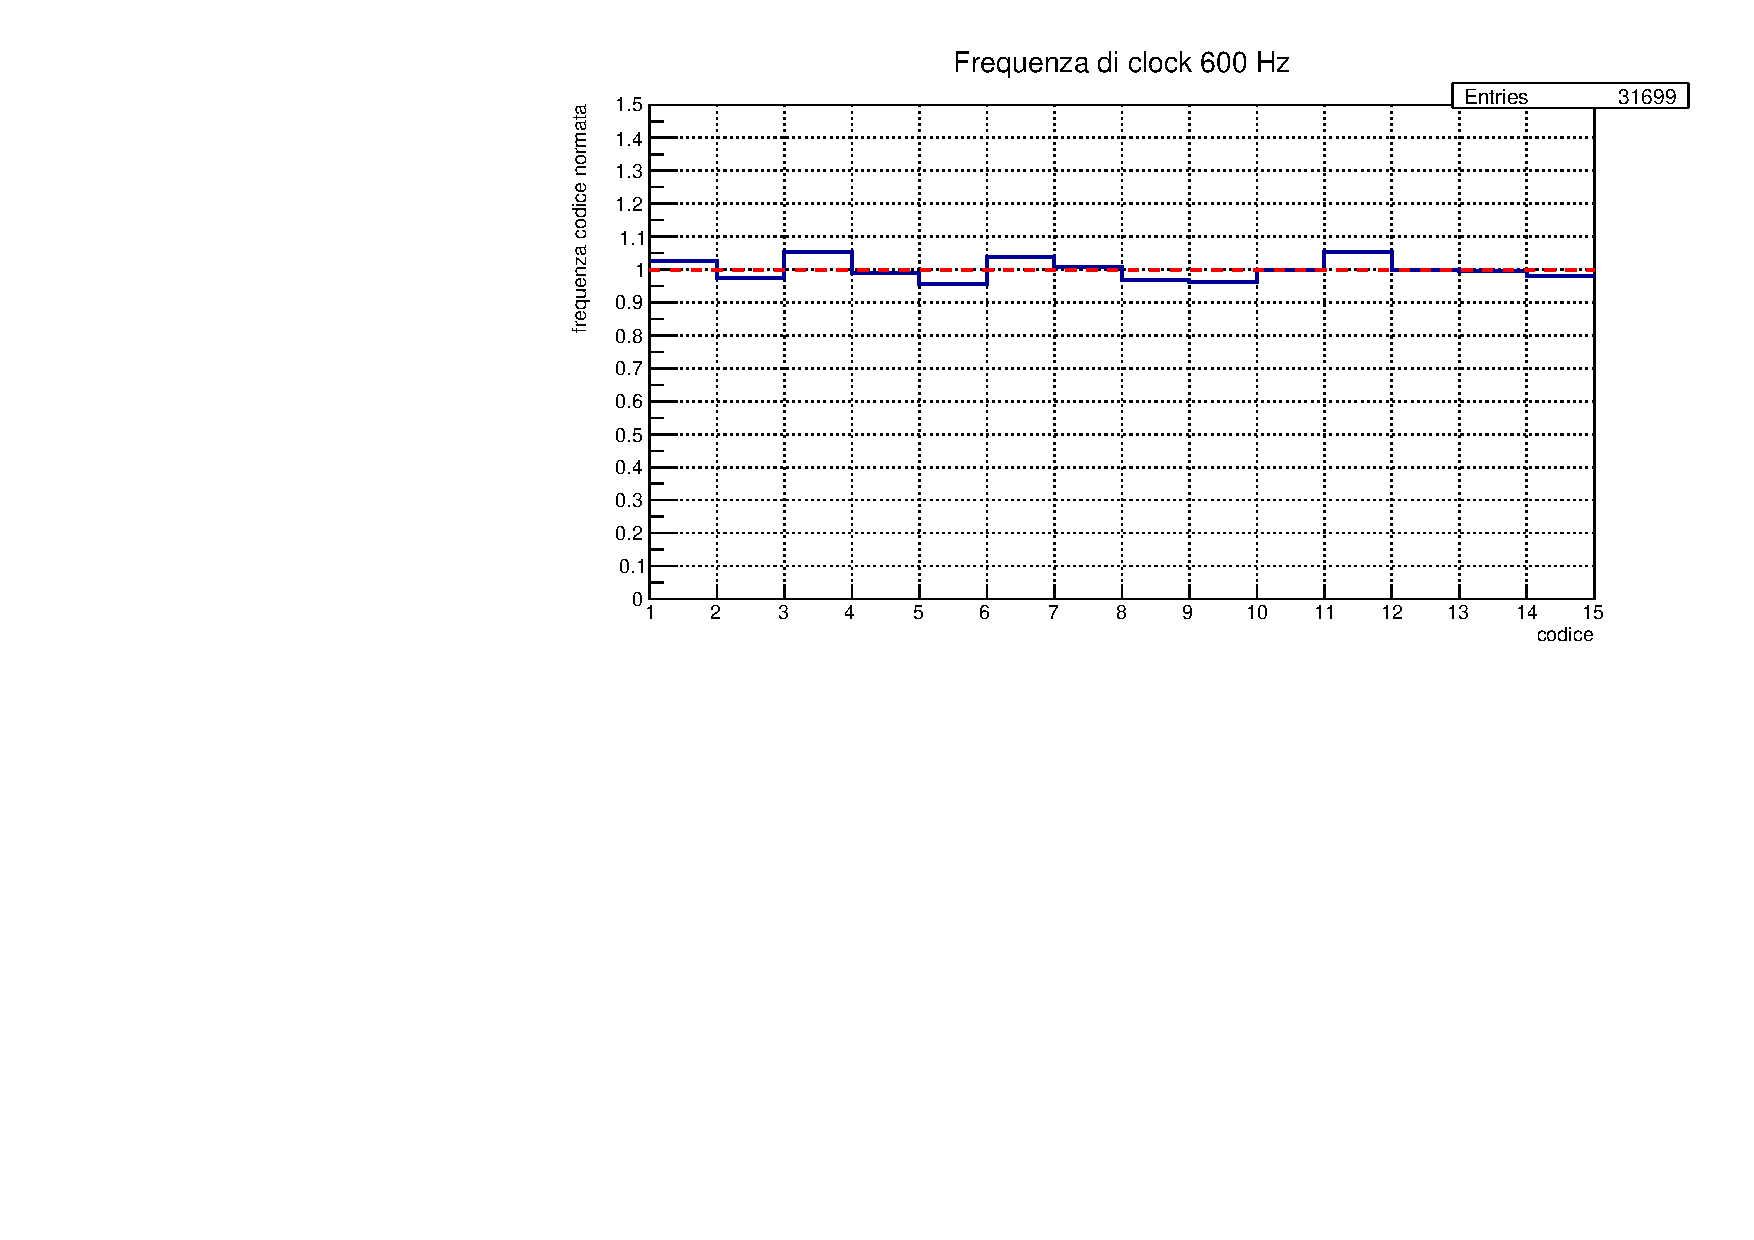
\includegraphics[width=0.48\textwidth]{analysis/output/dnl_2_600hz_bars.pdf}
\label{fig:graph_dnl_600_hz}



%3
\caption{$\sigma = 0.028$}
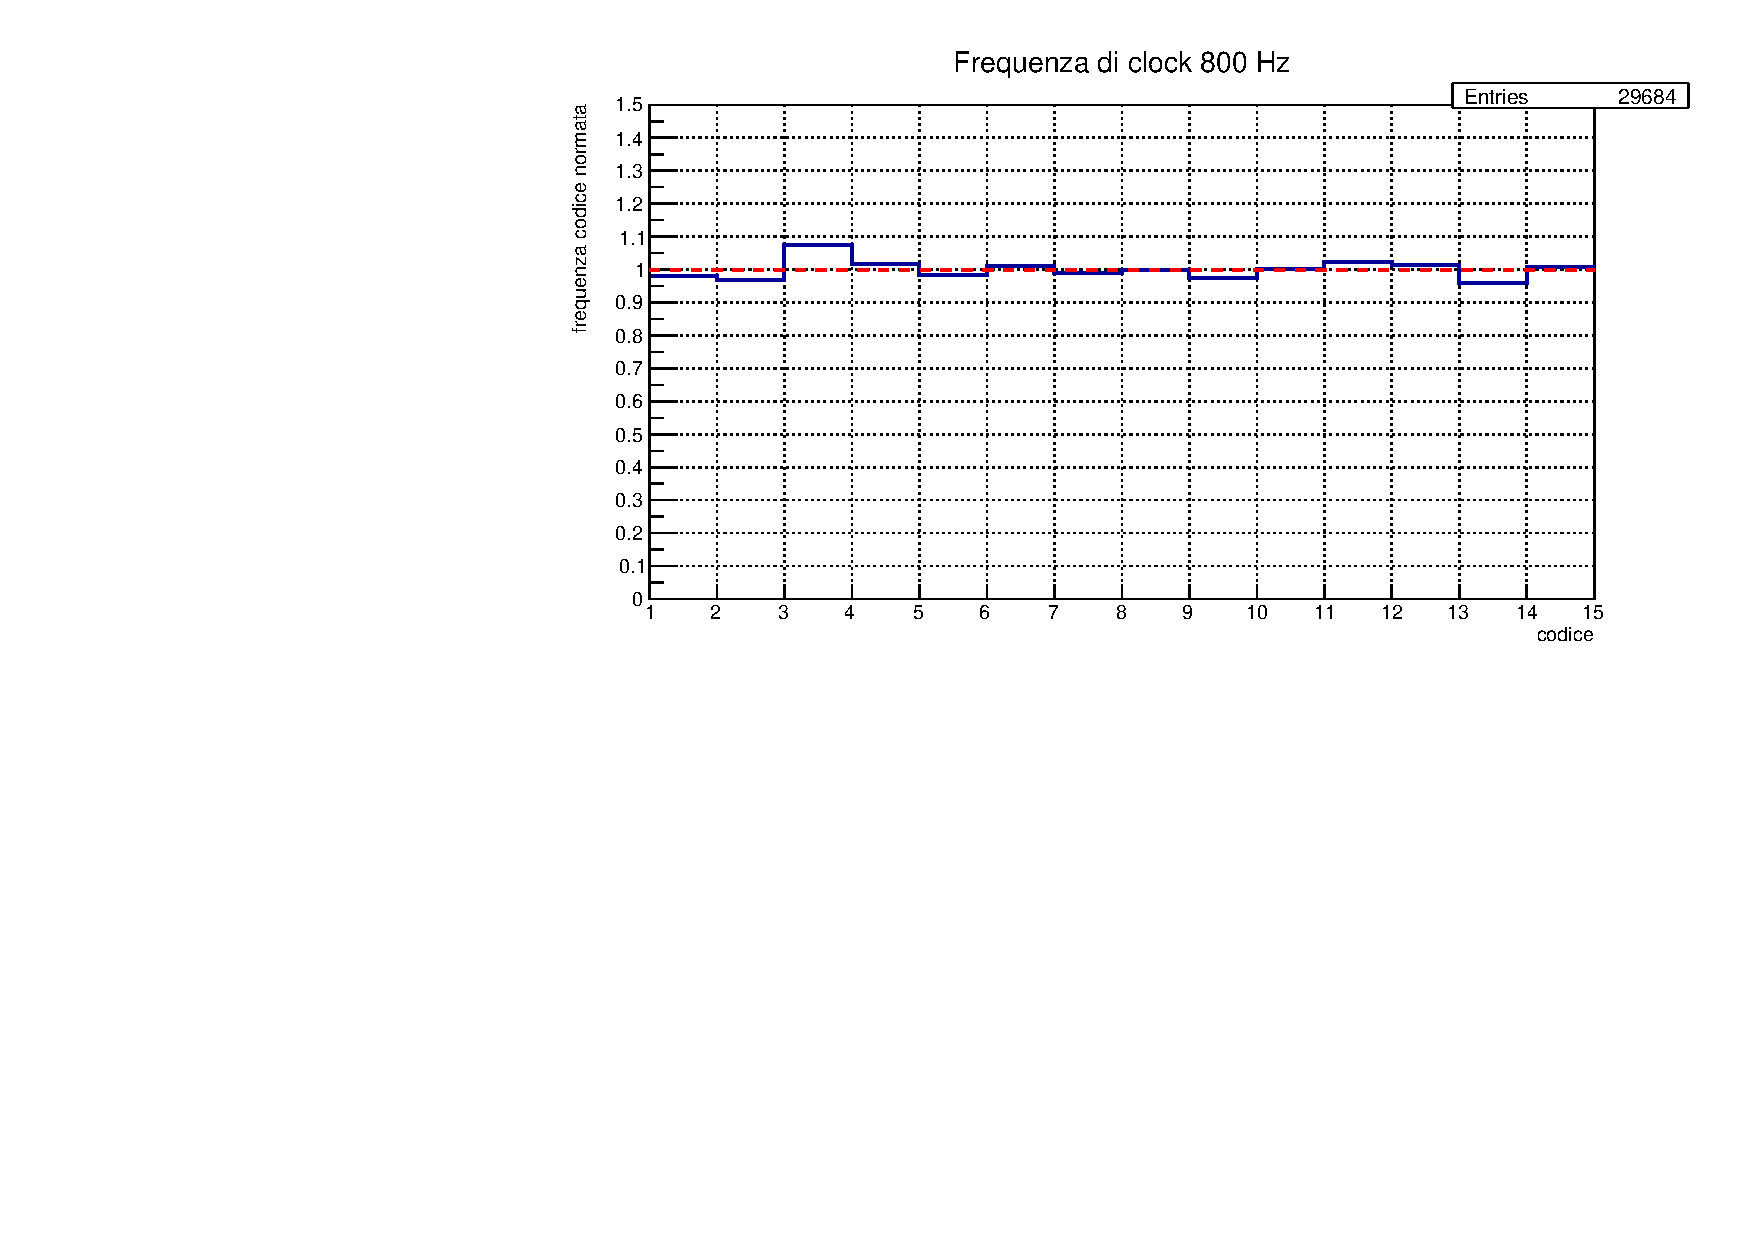
\includegraphics[width=0.48\textwidth]{analysis/output/dnl_3_800hz_bars.pdf}
\label{fig:graph_dnl_800_hz}
%4

\end{center}
\end{figure}

\begin{figure}[H]%[!ht]
\begin{center}

\caption{$\sigma = 0.030$}
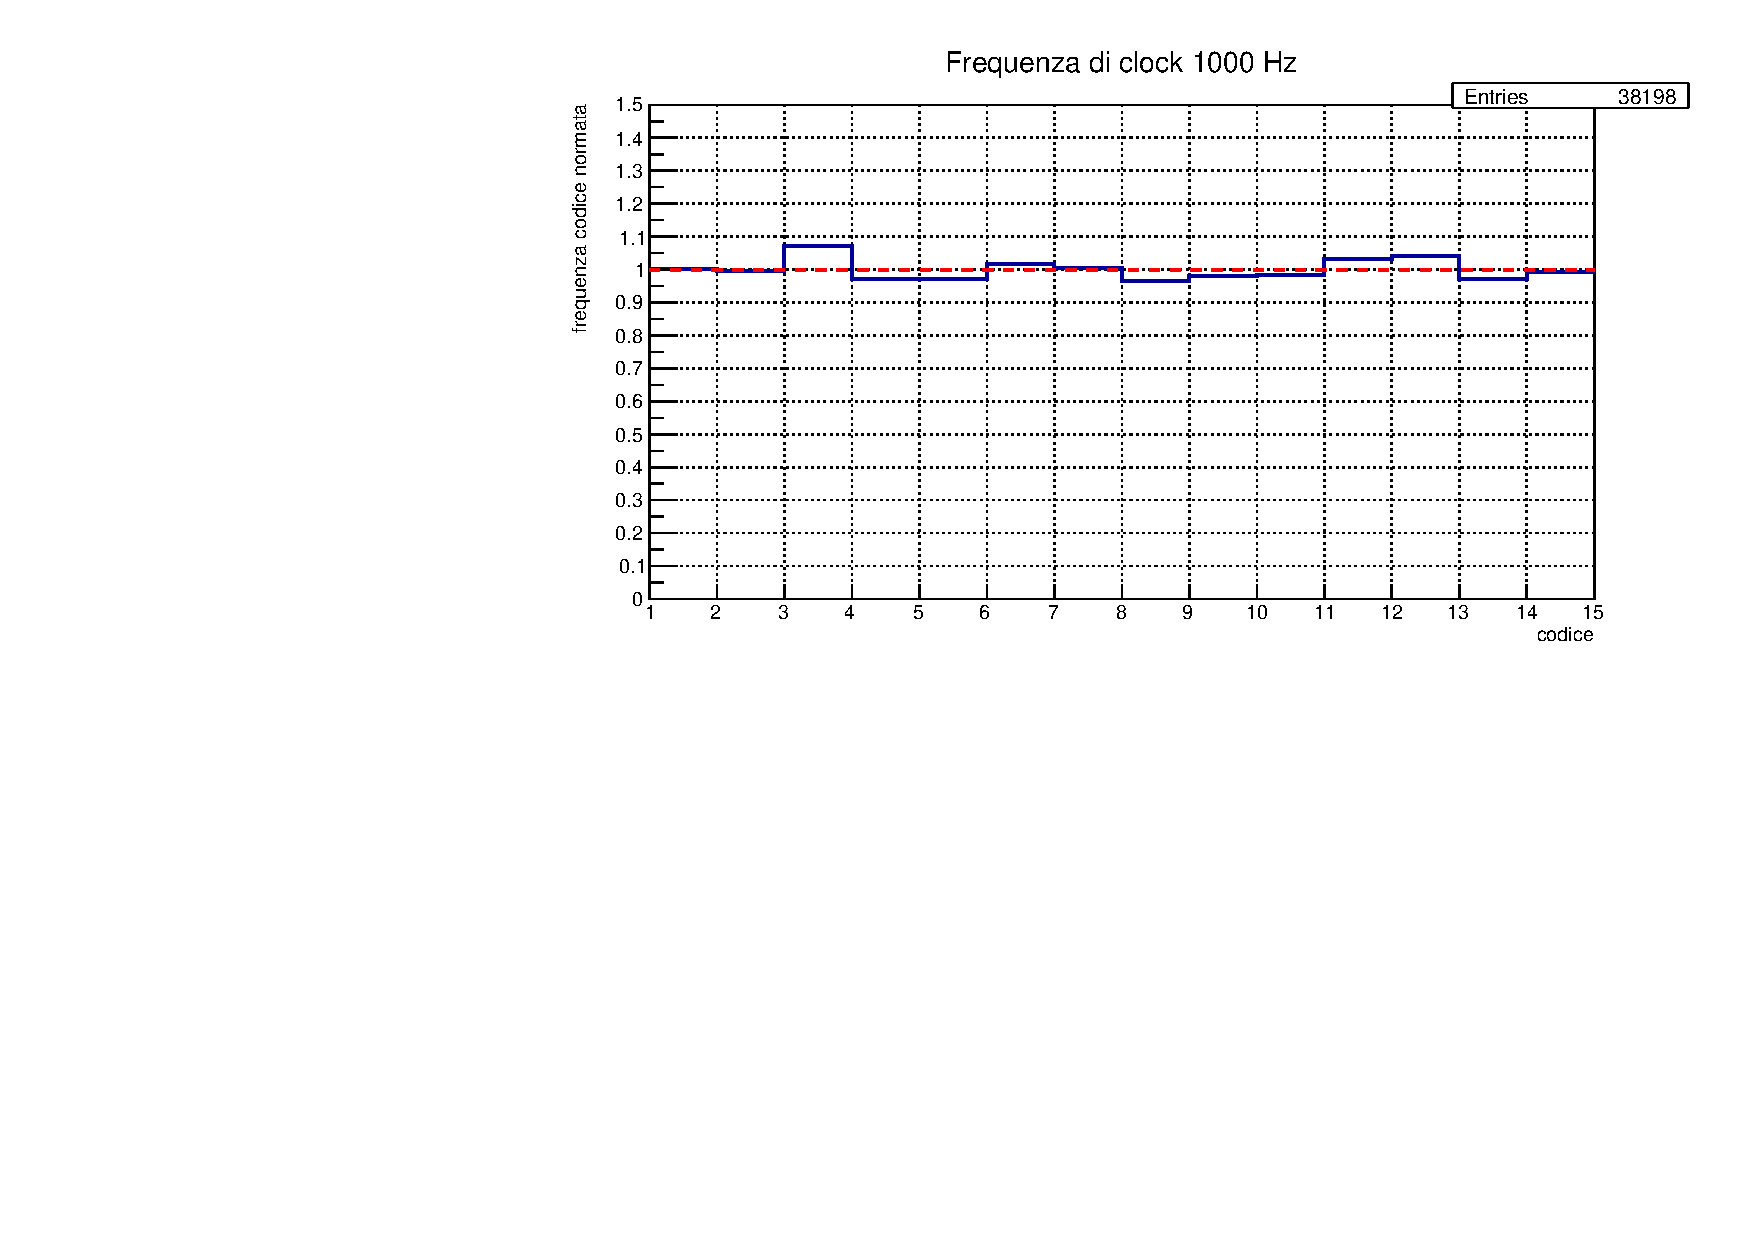
\includegraphics[width=0.48\textwidth]{analysis/output/dnl_4_1000hz_bars.pdf}
\label{fig:graph_dnl_1000_hz}

%5
\caption{$\sigma = 0.043$}
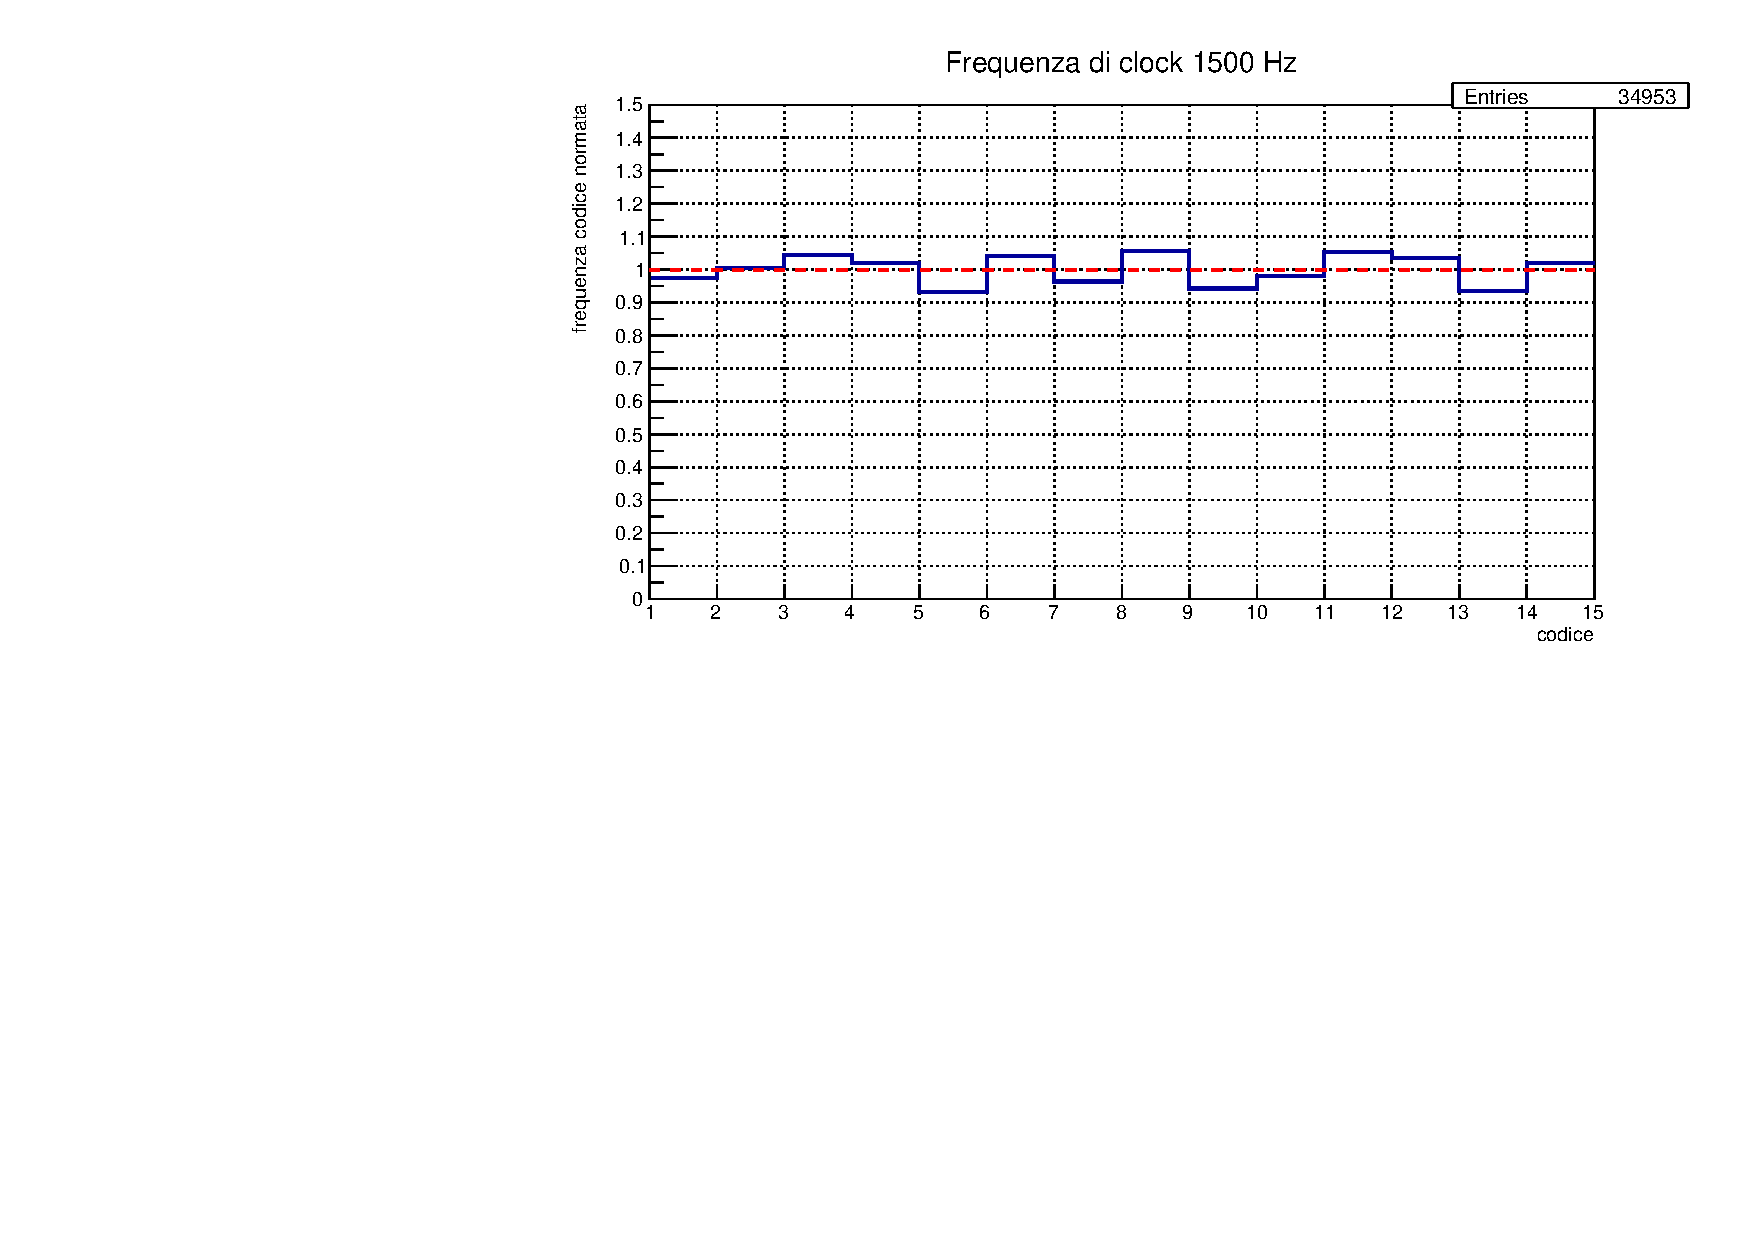
\includegraphics[width=0.48\textwidth]{analysis/output/dnl_5_1500hz_bars.pdf}
\label{fig:graph_dnl_1500_hz}
%6
\caption{$\sigma = 0.063$}
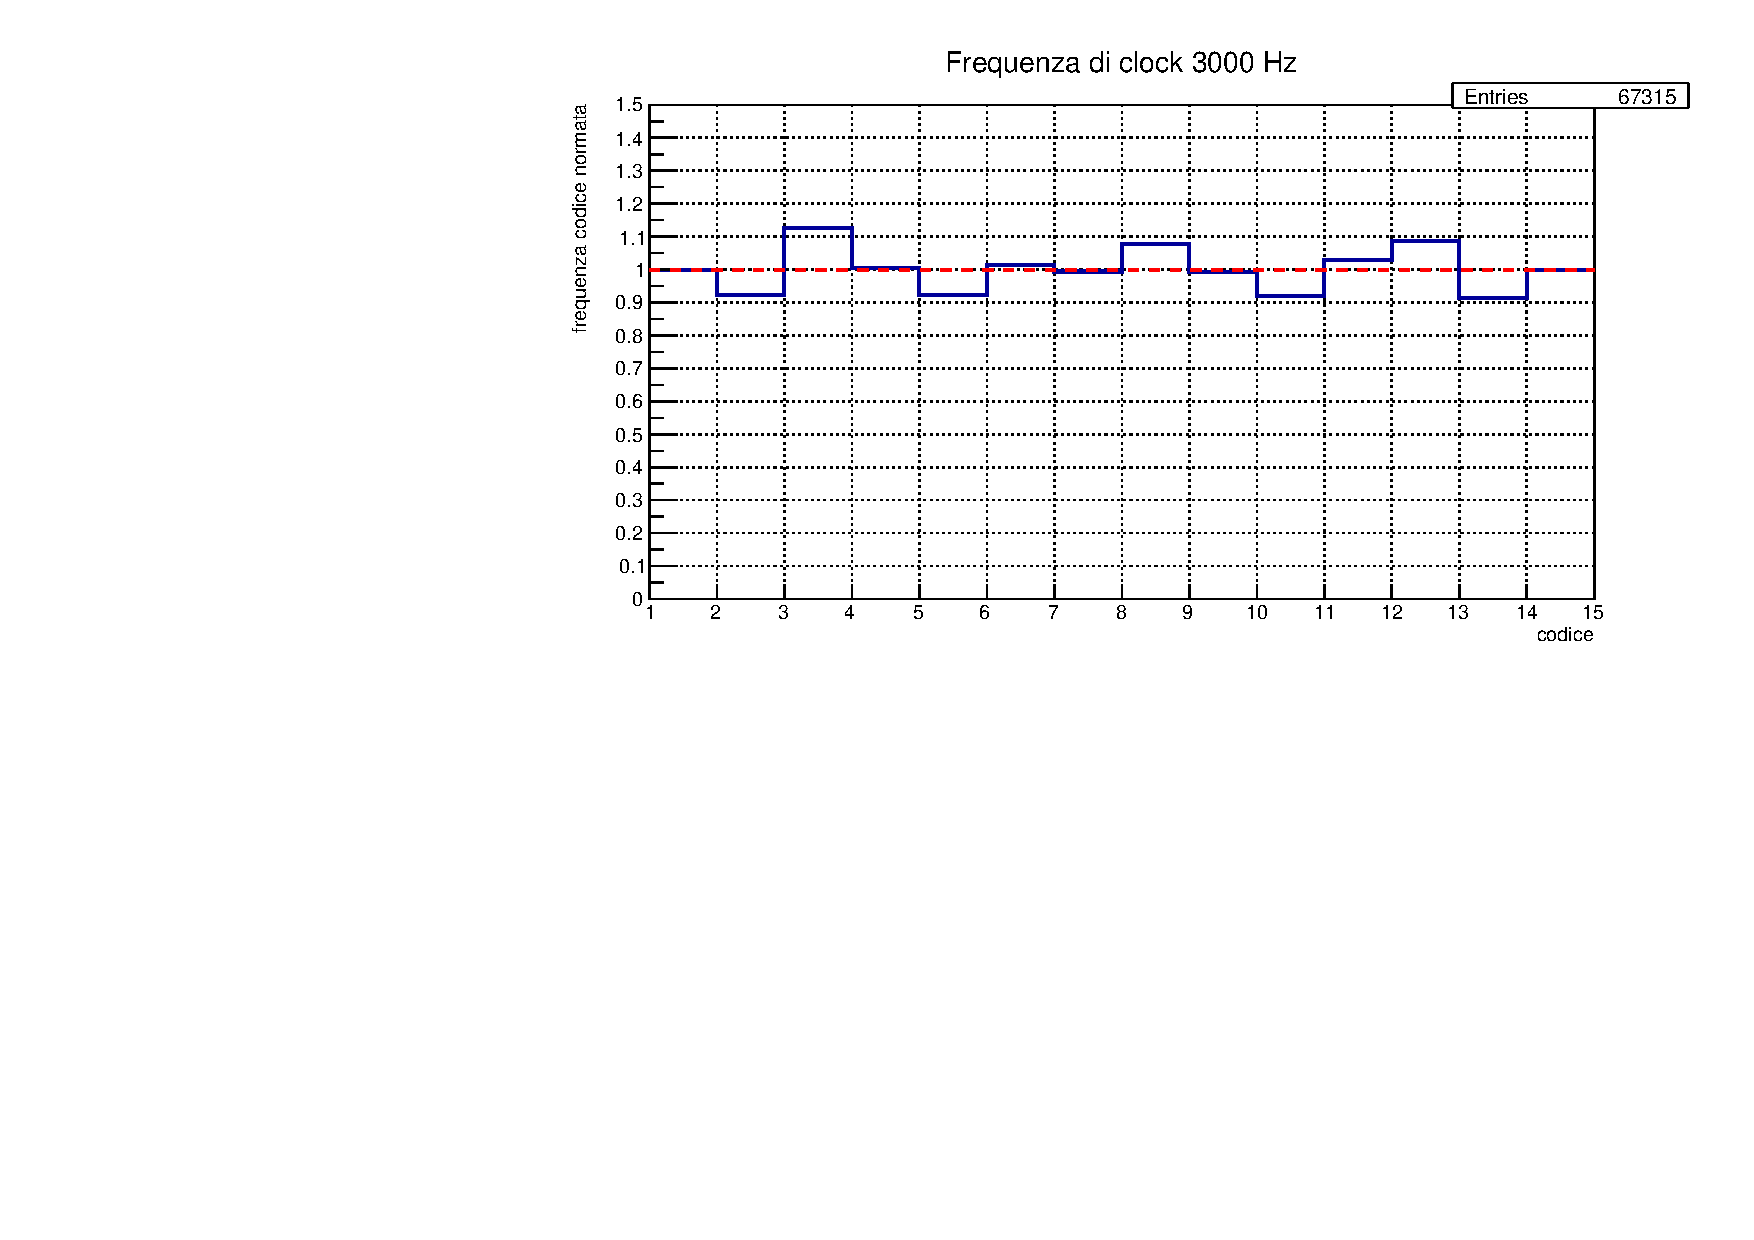
\includegraphics[width=0.48\textwidth]{analysis/output/dnl_6_3000hz_bars.pdf}
\label{fig:graph_dnl_3000_hz}
%7
\caption{$\sigma = 0.099$}
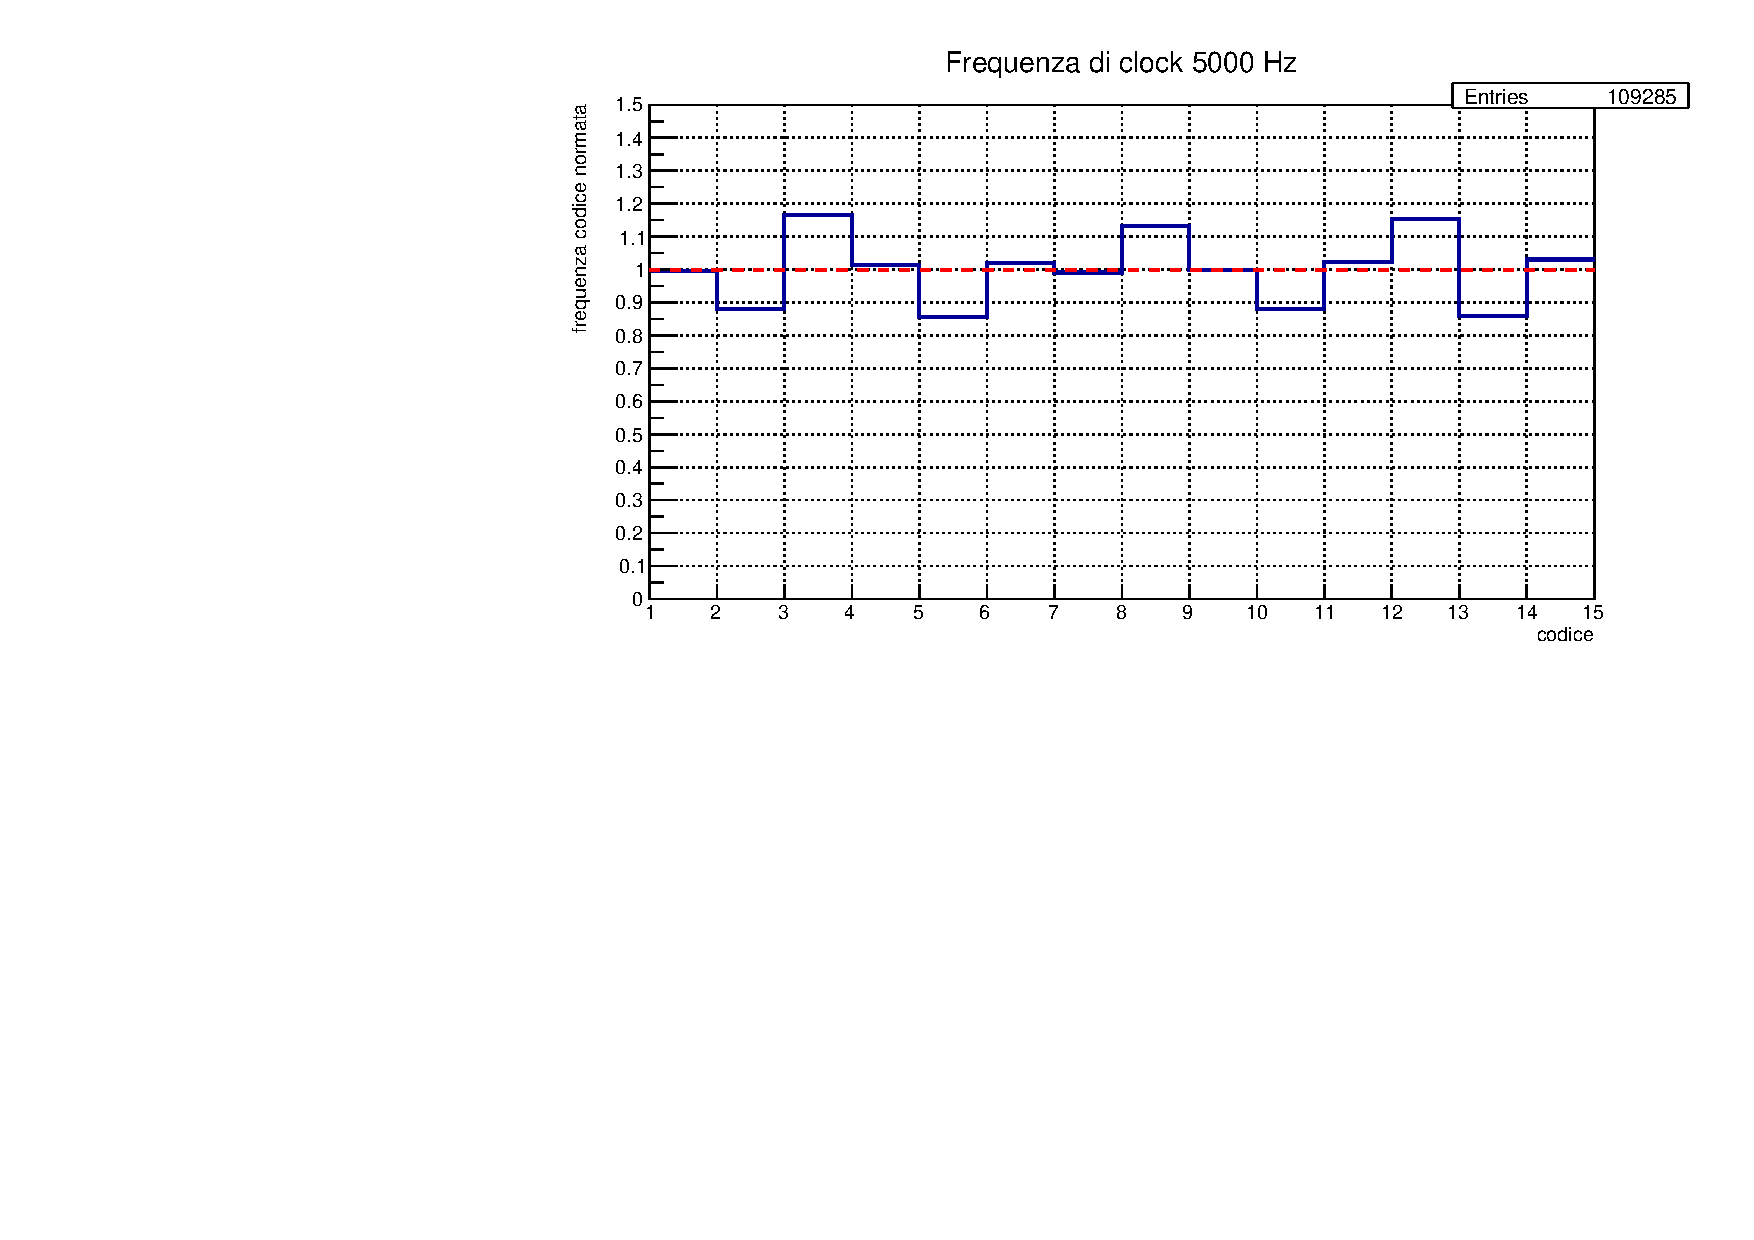
\includegraphics[width=0.48\textwidth]{analysis/output/dnl_7_5000hz_bars.pdf}
\label{fig:graph_dnl_5000_hz}
\end{center}
\end{figure}
\\
\begin{figure}[H]%[!ht]
\begin{center}


%8
\caption{$\sigma = 0.16$}
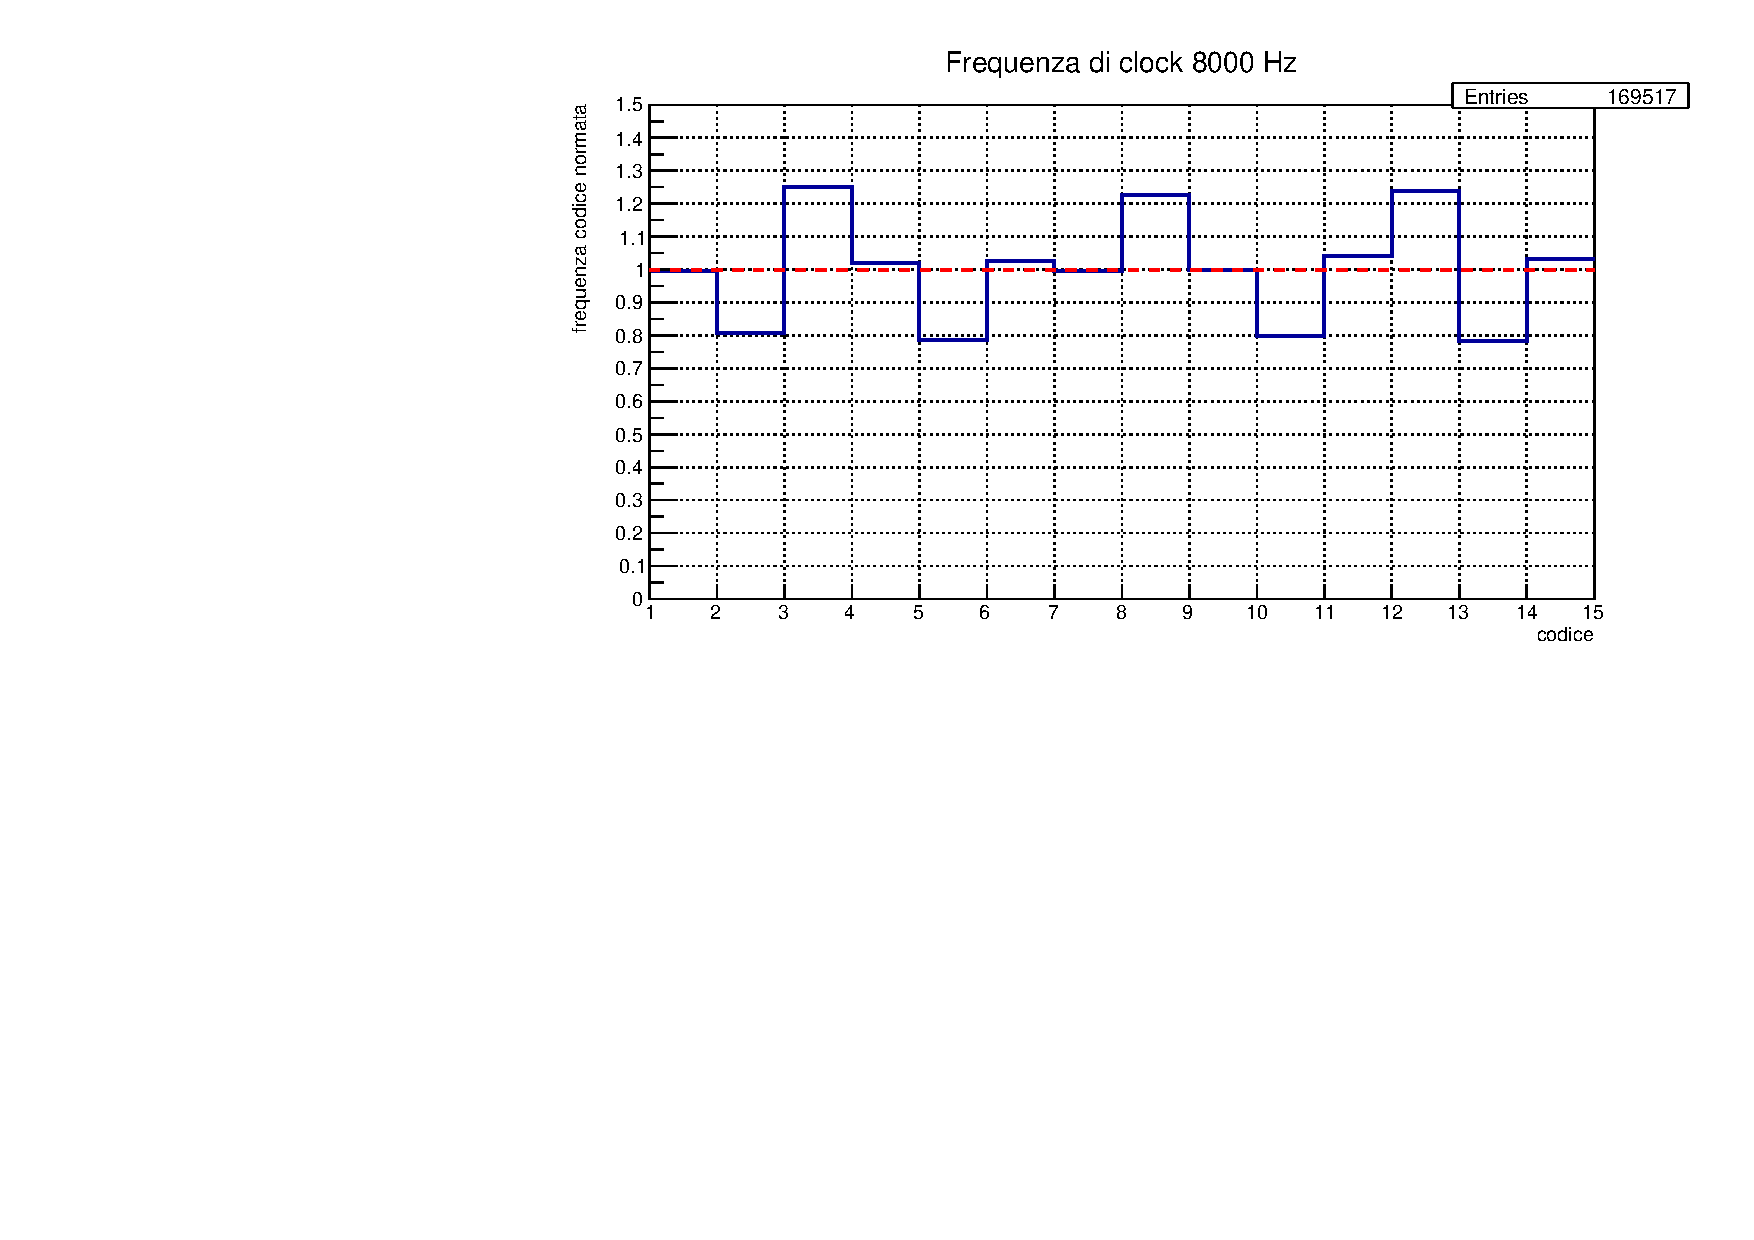
\includegraphics[width=0.48\textwidth]{analysis/output/dnl_8_8000hz_bars.pdf}
\label{fig:graph_dnl_8000_hz}

\end{center}
\end{figure}

Si analizza ora quanto emerge dagli istogrammi appena presentati. Innanzitutto per valutare in modo quantitativo lo scostamento complessivo dei conteggi dalla distribuzione uniforme, dopo aver normalizzato la media dei conteggi di ogni \textit{bin} a 1, è stata calcolata $\sigma$ cioè la deviazione standard della popolazione dei conteggi rispetto a questa media. Non è stato possibile analizzare l'esatta distribuzione poiché 14 codici (16 - \textit{underflow} e \textit{overflow}) non costituiscono una statistica sufficiente. La statistica dei conteggi per ciascun codice è invece notevole, in particolare è compresa tra 29684 registrazioni totali a 800 Hz fino a 169517 registrazioni totali a 8 KHz.

Si nota immediatamente come la linearità del dispositivo sia buona ($\sigma \sim 0.03$) solamente per frequenze di campionamento limitate. Dalla \textit{figura \ref{fig:graph_dnl_3000_hz}} alla \textit{figura \ref{fig:graph_dnl_8000_hz}}, infatti, si osservano scostamenti dei conteggi rispetto al valor medio normalizzato superiori al 10\%.
In particolare nella \textit{figura \ref{fig:graph_dnl_sigma}} si evidenzia come la deviazione standard $\sigma$ che si attesta su un valore di plateau a frequenze di \textit{clock} minori di 1 KHz, cominci ad aumentare fino a raggiungere circa il 16 \% del valore medio normalizzato quando il clock è pari a 8 KHz. Si osserva, inoltre, che la non linearità al crescere della frequenza è dovuta a eccesso o carenza di conteggi sempre negli stessi \textit{bin}, indipendentemente dalla frequenza e dallo sfasamento del segnale analogico da acquisire.

\begin{figure}[H]%[!ht]
\begin{center}
\includegraphics[width=0.50\textwidth]{analysis/output/dnl_sigma_pdf}
\caption{Letture mancanti}
\label{fig:graph_dnl_sigma}
\end{center}
\end{figure}

\subsection{Test inversione bit}
Dopo aver osservato che la non linearità che emerge al crescere della frequenza è dovuta ad un insieme ben determinato di codici preferenziali che risultano sopra / sotto la media normalizzata in tutte le acquisizioni, risulta naturale chiedersi se questo \textit{bias} sia introdotto dalla scheda Arduino oppure dai circuiti dell'ADC. Per rispondere a questa domanda è stata ripetuta l'ultima acquisizione con $f_{clock}$ = 8 KHz (\textit{figura \ref{fig:graph_dnl_8000_hz}}) scambiando tra di loro alcuni collegamenti tra le uscite dei J-K e gli ingressi digitali di Arduino e si è ottenuta la \textit{figura}  \textit{\ref{fig:graph_dnl_non_lin}}.
Osserviamo come i codici con maggiori ricorrenze abbiano seguito l'inversione dei collegamenti e ciò suggerisce che la scarsa linearità sia già presente alle uscite dei J-K; inoltre, essendo dipendente dalla frequenza di \textit{clock}, possiamo escludere come prima causa un'eccessiva diversità delle resistenze della rete R-2R, si tratta quindi probabilmente di un effetto dovuto alla dinamica dello stadio comparatore o ai J-K. 

%una R2R non perfettamente calibrata, condizione comprensibile a causa della limitata uguaglianza fra le resistenze impiegate.
%^^^ Questo non è possibile perché l'effetto dovrebbe essere indipendente dalla frequenza di clock.
\begin{figure}[H]%[!ht]
\begin{center}
\includegraphics[width=0.48\textwidth]{analysis/output/dnl_non_lin_8000hz_bars.pdf}
\caption{Presa dati con bit invertiti: $ 4->3, \ 3->2, \ 2->4 $}
\label{fig:graph_dnl_non_lin}
\end{center}
\end{figure}



%%%%%%%%%%%%%%%%%%%%%%%%%%%%%%%%%%%%%%%%%%%%%%%%%%%%%%%%%%%

\subsection{Valori mancanti}

\begin{figure}[H]%[!ht]
\begin{center}
\includegraphics[width=0.50\textwidth]{analysis/output/letture_mancanti.pdf}
\caption{In questo grafico si nota come il microcontrollore di Arduino salti periodicamente alcune letture}
\label{fig:missing}
\end{center}
\end{figure}

Durante una serie di acquisizioni effettuate a frequenze $f$ elevate rispetto a $f_{clock}$, con $f_{clock}$ multipla di $f$ si è osservato il fenomeno mostrato in \textit{figura \ref{fig:missing}}, cioè che il microcontrollore salta con una certa periodicità alcune letture. Questo potrebbe essere dovuto a qualche \textit{interrupt} legato a qualche libreria che sospende temporaneamente l'esecuzione del programma principale; per esempio si potrebbe trattare della libreria per la gestione della SPI che dialoga con il \textit{controller} della scheda di memoria. Questo effetto introdurrebbe sicuramente un \textit{bias} nelle verifiche di linearità qualora queste venissero effettuate con frequenze di clock multiple della frequenza del segnale oppure con sfasamento costante tra segnale e clock. Questo è uno dei motivi per cui il test di linearità discusso nei paragrafi precedenti è stato eseguito utilizzando uno \textit{sweep} in frequenza. Nelle condizioni sopra menzionate la distanza tra letture mancanti è nell'ordine di 50 ms. 



%%%%%%%%%%%%%%%%%%%%%%%%%%%%%%%%%%%%%%%%%%%%%%%%%%%%%%%%%%%%%
\section{Discussione dei risultati e conclusioni}
Nella presente relazione di laboratorio, dopo aver analizzato il comportamento di alcuni circuiti logici fondamentali, è stata affrontata la caratterizzazione di un ADC ad approssimazioni successive a 4 bit. 
\\

La verifica delle tavole di verità degli integrati logici ha dato esito positivo, con l'osservazione degli stati logici attesi; si è quindi proceduto con la misurazione delle caratteristiche di trasferimento in tensione degli integrati logici, che si sono dimostrate adeguate per ottenere una rigenerazione del segnale ad ogni porta, anziché un suo progressivo deterioramento. Si è però osservata una tensione di uscita in corrispondenza dello stato logico alto talvolta inferiore ai 5 V richiesti dallo standard TTL, non solo in presenza di carico sull'uscita, ma anche in condizioni di circuito aperto. Per la porta logica NOT è stato possibile calcolare in modo accurato anche il ritardo di propagazione del segnale logico t = (5.6428 $\pm$ 0.0007) ns mediante misurazione della frequenza di accordatura di un \textit{ring oscillator} realizzato collegando in cascata 7 inverter.
\\

È stata quindi affrontata la caratterizzazione dei circuiti logici sequenziali (flip-flop e registri) verificando non solo la corretta rappresentazione degli stati logici, ma anche la commutazione in prossimità dei fronti di \textit{clock} corretti (\textit{positive-edge} per quanto riguarda il registro a scorrimento e \textit{negative-edge} per quanto riguarda i flip-flop J-K). Nell'analizzare i circuiti logici di controllo del registro a scorrimento è stata misurata la durata del segnale asincrono di \textit{clear}, pari a $\Delta\tau$ = (46 $\pm$ 5) ns. Questo valore di durata è in realtà critico per il corretto funzionamento dell'ADC, in quanto la durata è pari alla somma tra il ritardo introdotto dal circuito logico ausiliario (vedere U8 in schema principale) e il tempo di reset del registro. Se qualche integrato logico necessitasse di un tempo maggiore per recepire il segnale di reset di quello impiegato dal registro, probabilmente emergerebbe un malfunzionamento. Tale evenienza in laboratorio non è però mai stata osservata.
\\

A questo punto è stata affrontata la caratterizzazione dei circuiti analogici, in particolare il DAC di tipo R-2R, il comparatore e il transistor di interfaccia. Per quanto riguarda il DAC, portando i singoli bit ai livelli logici opportuni, è stato possibile verificarne la linearità (p-value del test di adattamento di $\chi^2$ con una retta pari a 0.99) ottenendo una curva di calibrazione con coefficiente angolare m = (-0.211 $\pm$ 0.001) V e offset verticale q = (-0.01 $\pm$ 0.01) V. Si tratta di un risultato sufficiente, in relazione all'accuratezza che vorremo raggiungere con il nostro ADC. Per quanto riguarda in transistor di interfaccia tra l'uscita del comparatore e i circuiti digitali, è stata calcolata la caratteristica di trasferimento in tensione base-collettore, verificando la compatibilità del segnale in uscita con lo standard TTL e la rapidità del fronte di commutazione. 
\\

Si commentano ora i risultati delle misure effettuate sull'ADC a montaggio completato. Per prima cosa è stata effettuata la calibrazione dell'ADC utilizzando una tensione continua variabile regolata da un potenziometro, misurata con il multimetro, e registrando le soglie di commutazione tra un codice e il successivo. Innanzitutto si osserva che le soglie di commutazione dispongono di una certa isteresi: il passaggio da un codice a quello adiacente avviene a tensioni diverse se la rampa in ingresso risulta crescente o decrescente. Nel nostro caso la misurazione è stata svolta con una tensione decrescente in valore assoluto. In questo caso si osserva una compatibilità con il modello lineare pari a $\chi^2$ = 0.57, p-value = 0.99 mentre coefficiente angolare e l'offset risultano rispettivamente m = (-0.3092 $\pm$ 0.0001) V e q = (-0.02 $\pm$ 0.01) V. Questa volta si osserva non solo un $\chi^2$ maggiore, seppur comunque compatibile con il modello, considerando il livello di significatività usuale del 5 \%, ma soprattutto un range dinamico compresso rispetto alle tensioni TTL. Questo è dovuto da una tensione in uscita dai J-K più bassa della nominale già a circuito aperto. Il test Z di compatibilità con lo zero dell'offset questa volta riporta una non compatibilità: si ottiene un valore della variabile statistica Z = 2, p-value = 0.044, questa volta inferiore al livello di significatività del 5 \%, anche se con uno scostamento piccolo.
\\
%Range dinamico compresso vuol dire che anziché lavorare tra 0 e 5V l'ADC lavora tra 0 e 3.3 V circa. La colpa è dei J-K.

Si è quindi passati al campionamento di segnali analogici variabili nel tempo e alla verifica dapprima qualitativa, poi maggiormente quantitativa, del teorema di Nyquist-Shannon e del profilo di linearità del nostro ADC con il metodo della \textit{code density}. L'ADC ha dimostrato di essere in grado di ricostruire correttamente segnali analogici arbitrari e armoniche sinusoidali con frequenze fino alla metà della frequenza di campionamento, come previsto dal suddetto teorema; per effettuare queste acquisizioni la frequenza di \textit{clock} è stata impostata a 8 KHz. Lo studio della linearità con il metodo della \textit{code density} ha invece messo in luce delle discrepanze importanti rispetto alla distribuzione uniforme attesa per frequenze di clock superiori a 1.5 KHz comprendenti sequenze ben definite di bit che risultavano sistematicamente sopra o sotto il livello atteso. Dopo esserci assicurati che questo effetto non dipendesse dalla fase o dalla frequenza della rampa analogica impiegata impostando uno \textit{sweep}, abbiamo studiato la dipendenza della non linearità della frequenza di \textit{clock}, osservando una crescita costante da 1.5 KHz fino alla massima frequenza raggiunta, pari a 8 KHz. Questo ci porta ad affermare che la massima frequenza di campionamento a cui il nostro ADC opera in modo sufficientemente lineare è pari a 187 Hz, un valore estremamente sottodimensionato, se confrontato con quanto richiesto dalle applicazioni. È stato osservato che queste problematiche di linearità non dipendono dalla scheda a microcontrollore, ma proprio dal circuito dell'ADC. Uno dei principali colli di bottiglia del sistema preso in esame, quando si tenta di lavorare a frequenze più elevate, è probabilmente l'amplificatore operazionale \textit{LM741}. Infine, è stato osservato che la scheda a microcontrollore salta in modo piuttosto regolare delle letture, ma questo potrebbe essere risolvibile anche solo ottimizzando il suo \textit{firmware}.
\\

Nonostante queste problematiche emerse, l'obiettivo di questa esperienza di laboratorio - realizzare un ADC SAR a 4 bit - può considerarsi sicuramente raggiunto. Il \textit{design} può essere facilmente migliorato e scalato a maggiori risoluzioni senza eccessiva crescita della complessità e, in generale, i principi qui dimostrati possono essere implementati a scale di integrazione molto più elevata realizzando convertitori effettivamente utilizzabili per svariate applicazioni nelle quali non sia necessario raggiungere velocità di campionamento troppo elevate (in tal caso conviene orientarsi su convertitori \textit{pipeline}) o risoluzioni troppo elevate (in tal caso i \textit{Delta-Sigma} rimangono più indicati), ma dove sia richiesto un buon bilanciamento delle due, unito ad una complessità relativamente ridotta. Infine, si segnala una caratteristica che sarebbe particolarmente interessante da introdurre in futuro: si tratta della possibilità di utilizzare una tensione $V_{ref}$ di fondo scala dell'ADC diversa dal livello alto delle uscite dei J-K mediante uno stadio a transistor di tipo \textit{totem-pole}; questo consentirebbe di sfruttare al meglio il range dinamico disponibile.
\\

\begin{figure*}[t]%[t]
\centering
\begin{center}
\includegraphics[trim = {0 0 50 0}, width=1.40\textwidth, angle=90]{sch-simulations/digital/output/Schema_convertitore_completo.pdf}
\end{center}
\caption{Schema elettrico completo del convertitore ADC SAR 4 bit}
\label{fig:circuit_sarCompleteSchematic}
\end{figure*}



%%%%%%%%%%%%%%%%%%%%%%%%%%%%%%%%%%%%%%%%%%%%%%%%%%%%%%%%%%%%%
%% Appendice
%%%%%%%%%%%%%%%%%%%%%%%%%%%%%%%%%%%%%%%%%%%%%%%%%%%%%%%%%%%%%

\clearpage

\begin{appendices}

\section{Soglie di commutazione porta AND}

Riportiamo qui una misurazione svolta sulle porte AND contenute nell'integrato \textit{SN74LS08N} con l'obiettivo di stimare i valori delle soglie di commutazione degli ingressi. Per ricavare i grafici sottostanti uno dei due ingressi della porta AND è stato alimentato con un livello logico alto fisso, mentre all'altro ingresso veniva fornita una rampa simmetrica oscillante tra 0 e 5 V dal generatore di funzioni. L'oscilloscopio acquisiva sul primo canale tale rampa e sul secondo canale l'uscita della porta logica. È stato così possibile osservare e misurare tramite cursori, che la commutazione verso l'alto avviene quando l'ingresso supera la soglia ${\Delta}V_1$ = (1.02 $\pm$ 0.05) V, mentre la commutazione verso il basso avviene quando l'ingresso scende sotto ${\Delta}V_1$ = (0.84 $\pm$ 0.05) V. Si osserva quindi una certa isteresi; seppur minima e in una regione del grafico particolarmente rumorosa.

\begin{figure}[H]%[!ht]
\begin{center}
\includegraphics[width=0.48\textwidth]{analysis/output/and-switching.pdf}
\caption{Soglie di commutazione porta logica AND}
\label{fig:AND-switching}
\end{center}
\end{figure}



\begin{figure}[H]%[!ht]
\begin{center}
\includegraphics[width=0.48\textwidth]{analysis/output/and-switching2.pdf}
\caption{Soglie di commutazione porta logica AND, con cursori}
\label{fig:AND-switching-cursors}
\end{center}
\end{figure}

\section{Alimentazione dei circuiti e scheda ausiliaria}
I circuiti descritti in questa relazione per il loro funzionamento hanno richiesto tre livelli di tensioni di alimentazione: $\pm$ 15 V per lo stadio analogico contenente il \textit{sample} \& \textit{hold} e gli amplificatori operazionali e +5 V per l'alimentazione degli integrati TTL. La tensione duale era fornita dall'alimentatore GW-Instek GPS-4303 per la cui descrizione, così come quella degli altri strumenti, si rimanda alla relazione di elettronica analogica ed è stata misurata ottenendo i seguenti valori: $V_+$ = (15.1 $\pm$ 0.1) e V $V_-$ = (-14.9 $\pm$ 0.1) V. La tensione TTL, invece, è stata fornita da una scheda ausiliaria progettata dal Dipartimento di Fisica contenente al suo interno, oltre agli switch e ad una serie di LED con ingressi in standard TTL, un regolatore di tensione lineare LDO (low dropout) che genera la tensione + 5 V a partire dalla + 15 V.

\section{Tabella calibrazione DAC}

\centering
\begin{tabular}{cc}
binario & V $ \pm 0.1 \ V $ \\ \hline
0000    & 0.0                          \\
0001    & -0.3                       \\
0010    & -0.6                       \\
0011    & -0.9                       \\
0100    & -1.2                       \\
0101    & -1.6                       \\
0110    & -1.9                       \\
0111    & -2.2                       \\
1000    & -2.5                       \\
1001    & -2.8                       \\
1010    & -3.1                       \\
1011    & -3.4                       \\
1100    & -3.7                       \\
1101    & -4.0                       \\
1110    & -4.3                       \\
1111    & -4.6
\vspace{5 mm}
%\caption{}
\label{tab:calibrazione_dac}
\end{tabular}


\section{Tabella calibrazione ADC}

\begin{tabular}{cc}
binario & $V_{inf}  \pm 0.1 \ V$ \\ \hline
1111    & -3.2                  \\
1110    & -3.0                  \\
1101    & -2.7                  \\
1100    & -2.5                  \\
1011    & -2.3                  \\
1010    & -2.1                  \\
1001    & -1.9                  \\
1000    & -1.7                  \\
0111    & -1.5                  \\
0110    & -1.3                  \\
0101    & -1.0                  \\
0100    & -0.8                  \\
0011    & -0.7                  \\
0010    & -0.5                  \\
0001    & -0.2                  \\
0000    & 0.0
\vspace{5 mm}
%\caption{}
\label{tab:calibrazione_adc}
\end{tabular}


\end{appendices}

%%%%%%%%%%%%%%%%%%%%%%%%%%%%%%%%%%%%%%%%%%%%%%%%%%%%%%%%%%%%%
%% Indice e Bibliografia 
%%%%%%%%%%%%%%%%%%%%%%%%%%%%%%%%%%%%%%%%%%%%%%%%%%%%%%%%%%%%%

\clearpage
\newpage

\tableofcontents % Indice


\printbibliography % Bibliografia

\end{document}   

